%!TEX program = xelatex
%
% Thinking of Thinking
% An introductory logic textbook by Masahiro Yamada. 
%
\documentclass[table]{logicbook}
\usepackage{logicfonts}
\usepackage{logic_commands}


%comment following for final version
%\usepackage[notcite]{showkeys}

%*********************************
%DIRECTORIES
%*********************************
\newcommand{\chdir}{chapters}
\newcommand{\ttdir}{\chdir/TruthTables}
\newcommand{\exdir}{\chdir/exercises}
\newcommand{\prdir}{\chdir/proofs}
\newcommand{\supdir}{\chdir/sup}
\newcommand{\bibdir}{\chdir/bib}

%*********************************
%HELPER COMMANDS
%*********************************
%you need to install lbhelper and also allow
%executing external commands through LaTeX.

\newcommand{\plsh}[1]{\input{|"lbhelper -f #1"}}% (sentential logic formula)
\newcommand{\plshn}[1]{\input{|"lbhelper -f -m=false #1"}}% (sentential logic 
%formula)
\newcommand{\plshs}[1]{\input{|"lbhelper -seq '#1'"}} %SL sequent
\newcommand{\plshsn}[1]{\input{|"lbhelper -m=false -seq '#1'"}} %SL sequent
\newcommand{\pltt}[1]{\input{|"lbhelper -tt #1"}} %truth table
\newcommand{\plstf}[1]{\input{|"lbhelper -stf #1"}} %syntax tree full
\newcommand{\plsts}[1]{\input{|"lbhelper -sts #1"}} %syntax tree simple
\newcommand{\plshp}[1]{\input{|"lbhelper -p -f #1"}}% (predicate logic formula)
\newcommand{\plshpn}[1]{\input{|"lbhelper -p -m=false -f #1"}}% (predicate logic 
%formula)
\newcommand{\lbh}[1]{\input{|"lbhelper #1"}}%call lbhelper 


\begin{document}
\newpage
\title{Introduction to Formal Logic}
\author{Masahiro Yamada}
\date{}

\frontmatter \newpage
\maketitle


\textbf{About This Book}

This is material I have used to teach introductory level formal logic at Pomona 
College. The material is broken down to be doable in a 15 week semester with two 
sessions per week.

The proof system used in the book is the one Gentzen presents in his 
\citeyearpar{Gentzen1936}.

You can get exercises and some handouts at:

\url{https://adamay909.github.io/logicbook/}

There is a proof checker available at:

\url{https://adamay909.github.io/logicTools/}

The LaTeX sources are available at:

\url{https://github.com/adamay909/logicbook}

\vskip 2em

\textbf{License}

The book, exercises, answer keys are licensed under the Creative Commons 
Attribution-ShareAlike 4.0 license
(\url{https://creativecommons.org/licenses/by-sa/4.0/}).





\setcounter{tocdepth}{1}
\tableofcontents

\newpage
\mainmatter

\part{Formal Logic}

\chapter{Logical Connectives in English}\label{ch:NaturalLanguage}

\section{Sentences}\label{sec:SL-intro}


In this chapter we will be looking at logical connectives in a natural language,
 in particular English.  Just exactly what logical connectives are will be 
 explained as we proceed.


\subsection{Sentences}

Our natural languages have components that can be combined to form larger 
linguistic units. For example, we can combine words to form sentences.  
Sentences to form paragraphs. In this part of our class, our interest is in a 
certain type of sentences. Which type? In English there is an easy way of 
isolating the type of sentence we are interested in: prefixing them with `It is 
true that' results in a grammatically correct sentence. Let me explain:

In English, the following are all sentences:

\begin{itemize}

 \item Grass is always greener on the other side.

 \item Is your neighbor's lawn greener than yours?

 \item Let's go check out our neighbor's lawn.

\end{itemize}

If you prefix each of these with `It is true that', you get:

\begin{itemize}

 \item It is true that grass is always greener on the other side.

 \item It is true that is your neighbor's lawn greener than yours?

 \item It is true that let's go check out our neighbor's lawn.

\end{itemize}

Of the latter group, only the first is a grammatically correct sentence of 
English so the only of interest to us in the former group is the first sentence.  
It is the only one of the three that grammatically speaking could be true or 
false in the sense that English grammar allows us to say that it is true by 
simply prefixing `it is true that' to it.  From now on, when we speak of 
sentences, we only mean such sentences.  The following are all sentences:

\begin{itemize}

 \item One plus one is two.

 \item Vanilla ice cream is delicious.

 \item I don't like steak to be well done.

 \item The Earth is flat.

 \item If the Mongol Empire had not expanded into Eastern Europe, Russia as we 
  know it would not have existed.

 \item Free will is an illusion.

 \item The Middle Ages ended with the fall of Constantinople.

 \item It is morally impermissible to tell a lie.

\end{itemize}

Each of these results in a grammatically correct sentence of English when 
prefixed with `it is true that':

\begin{itemize}

 \item It is true that one plus one is two.

 \item It is true that vanilla ice cream is delicious.

 \item It is true that I don't like steak to be well done.

 \item It is true that the Earth is flat.

 \item It is true that if the Mongol Empire had not expanded into Eastern Europe, 
  Russia as we know it would not have existed.

 \item It is true that free will is an illusion.

 \item It is true that the Middle Ages ended with the fall of Constantinople.

 \item It is true that it is morally impermissible to tell a lie.

\end{itemize}

That we can prefix a sentence with `it is true that' and get a grammatically 
correct sentence means just that: the resulting sentence is grammatically 
correct. It does not mean that the sentence is true. For instance, in the list 
just given, some are true, others definitely false, some controversial, and in 
some cases it might even be unclear whether what's being asserted really is the 
sort of thing that can be true or false. But that does not matter for our 
purposes.\footnote{English has a rather simple grammar that allows just 
 prefixing a sentence with `it is true that' to yield a grammatically correct 
 sentence. Your native tongue might not allow anything this simple to isolate 
 the sentences we are interested in. When in doubt about which of the sentences 
in your native tongue are of interest, the simple solution is to translate them 
into English and see.} 

\subsection{Connectives}

The prefix `it is true that' is a device that we can use to form a new sentence 
out of another sentence. There are other such devices. Some of them can take two 
sentences and form a new sentence out of them. We call devices that can be used 
to form new sentences out of other sentences \emph{connectives}. For example, 
`it is true that' is a connective. There are also others.

For example, take the following two sentences:

\begin{slist}
 \item Henry VIII was surrounded by men named Thomas.\footnote{Here are some of 
  the people who were at one point or another of great influence under Henry 
 VIII: Thomas Wolsey, Thomas More, Thomas Cromwell, Thomas Boleyn, Thomas Howard, 
Thomas Seymour, Thomas Cranmer, Thomas Wriothesley.} 

 \item Henry VIII was too lazy to remember names.
\end{slist}

These can be combined in various ways to form more complex sentences:

\begin{slist}

\item Henry VIII was surrounded by men named Thomas \emph{and} Henry VIII was 
 too lazy to remember names.


\item Henry VIII was surrounded by men named Thomas \emph{because} Henry VIII 
 was too lazy to remember names.

\end{slist}

We can also take a single sentence and turn it into another sentence by, for 
instance, adding a prefix:

\begin{slist}
\item \emph{It is not true that} Henry VIII was surrounded by men named Thomas.

\item \emph{Anne believes that} Henry VIII was surrounded by men named Thomas.
\end{slist}

Notice that the results are all sentences in our sense since they can all be 
prefixed with `it is true that'. For example:

\begin{slist}

\item It is true that Henry VIII was surrounded by men named Thomas \emph{and} 
 Henry VIII was too lazy to remember names.

\item It is true that Henry VIII was surrounded by men named Thomas 
 \emph{because} Henry VIII was too lazy to remember names.

\item It is true that \emph{it is not true that} Henry VIII was surrounded by 
 men named Thomas.

\item It is true that \emph{Anne believes that} Henry VIII was surrounded by men 
 named Thomas.

\end{slist}

So `and', `because', `it is not true that', and `Anne believes that' are all 
connectives. There are many more connectives in English. Sentences that are 
formed from other sentences through the use of connectives are called 
\emph{compound} sentences. Sentences 3 through 10 are all compound sentences. 

We will only be interested in some connectives. Of the ones we have seen so far, 
we will be interested in `and' and `it is not the case that' because these  
qualify as logical connectives. But we will not be interested in `because' and 
`Anne believes that' because these do not qualify as logical connectives. Just 
why that is so will become clearer as we move along. 

Here is some terminology that we will be using:
\begin{itemize}

 \item We will be speaking of \emph{atomic} sentences and \emph{compound} 
  sentences. Atomic sentences are the sentences that we use as basic building 
  blocks for forming compound sentences. Compound sentences are formed by 
  manipulating atomic sentences using connectives (like combining them with the 
  word `and', or prefixing a sentence with `it is not the case that').  

\item We will speak of \emph{sentences} to cover both atomic and compound 
 sentences.

 \item If a sentence is true, we will say that its \emph{truth value} is true.  
  If the sentence is not true, we will say that its truth value is false.

\end{itemize}

Just like atoms that chemistry talks about are not at all simple, atomic 
sentences need not be simple sentences.  But when we designate a sentence as 
atomic, we will disregard any internal structures that the atomic sentence might 
have---in particular, we disregard whether they might themselves have parts that 
are sentences. So calling a sentence `atomic' does not say anything about the 
sentence except that we are treating it as a basic building block out of which 
we form other sentences. What the sentence says might be highly complex.






\section{Necessary and Sufficient Conditions}

We will often be talking about necessary and sufficient conditions for this and 
that to be the case.

A \emph{necessary condition} is a condition that must be met for something to be 
the case.  For instance, in order to vote in congressional elections in the U.S.  
you must be 18 years or older. So being 18 years or older is a necessary 
condition for it to  be the case that you are eligible to vote in congressional 
elections.  The standard way to express a necessary condition in this course 
will be:

\begin{center}
 \blank only if \blank

\end{center}

The blanks need to be filled in so that the result is a grammatically correct 
sentence of English. For instance:

\begin{center}
 You are eligible to vote in U.S. congressional elections \bemph{only if} you 
 are 18 years or older.
\end{center}

The bold face is just so you see the `only if'. It will usually not be bolded or 
otherwise emphasized.


A \emph{sufficient condition} for something to be the case is a condition that 
suffices to make it the case but is not necessary. For instance, suppose that 
satisfactorily passing a third semester French course suffices to meet your 
school's foreign language requirements for graduation but that it is not 
necessary to pass a third semester French course.  You could take Chinese, 
Arabic, etc.  Maybe there are even ways of avoiding a language course.  The 
standard way of expressing a sufficient condition in this course will be:

\begin{center}
 \blank if \blank
\end{center}

For instance:

\begin{center}
 You meet the foreign language requirement \bemph{if} you satisfactorily pass a 
 third semester French course.
\end{center}

Some conditions are both necessary and sufficient. The standard way of 
expressing that is:

\begin{center}
 \blank if, and only if, \blank
\end{center}

For instance, 

\begin{center}
 You meet the mathematical and formal reasoning requirement at your school 
\bemph{if, and only if,} you take a course in mathematics, computer science, 
formal logic, or statistics.  \end{center}

`if, and only if,' is often abbreviated as `iff.', like this:

\begin{center}
 You meet the mathematical and formal reasoning requirement at your school 
\bemph{iff.} you take a course in mathematics, computer science, formal logic, 
or statistics.  \end{center}



\section{Simple Symbolization}\label{sec:SL-compound}

Let us use the following sentences as our atomic sentences:

\begin{slist}

\item Snow is white.

\item The moon is made of cheese.

\item Marco Polo visited China.

\item Marco Polo met people who had visited China.

\item Marco Polo completely made up his story.

\end{slist}

Until further notice, these are the only atomic sentences there are. 

The following are all compound sentences that can be formed from these atomic 
sentences.  I am putting brackets around the sentences making up the compound 
sentence. The brackets can also be nested when compound sentences are combined 
to form further compound sentences.

\begin{slist}
 
\item \pp{Snow is white} and \pp{the moon is made of cheese}.

 \item It is not the case that \pp{the moon is made of cheese}.

 \item Either \pp{Marco Polo visited China} or \pp{Marco Polo met people who had 
  visited China}.

\end{slist}


Spelling out the sentences can get tedious quickly so let's use upper case Roman 
letters (A, B, C, ...) to represent sentences. For example,

\begin{lkey*}

\item[A] Snow is white.

\item[B] The moon is made of cheese.

\item[C] Marco Polo visited China.

\item[D] Marco Polo met people who visited China.

\item[E] Marco Polo completely made up his story.

\end{lkey*}

With these symbolization keys, we can rewrite the compound sentences above as:

\begin{slist}

 \item A and B.

 \item It is not the case that B.

 \item Either C or D.

\end{slist}

We can also produce more complex sentences:

\begin{slist}

\item \pp{A and \pp{C or D}} or \pp{B and \pp{\pp{it is not the case that C} and 
 E}}
 .

\end{slist}

The brackets are used to make clearer what goes with what. Notice that if we had 
stipulated that only A through D are atomic sentences, the last sentence would 
not be one of the compound sentences that can be formed: it needs E and that 
would not be available as an atomic sentence. So changing which sentences are 
the atomic sentences makes a difference to what compound sentences can be 
formed.  That is why it is important to be explicit about what the atomic 
sentences are. 



\section{Logical Connectives}

Let's take a closer look at the connective `and'. It takes two sentences and 
produces a third one. Let's use the following symbolization keys:

\begin{lkey*}

\item[A]  Henry VIII was surrounded by men named Thomas. 

\item[B]  Henry VIII was too lazy to remember names.

\end{lkey*}

A and B are both sentences. That means either can be true or false. They could 
be both true, both false, or one of them true and the other false. That gives us 
four possibilities. For each possibility, we can say whether \pp{A and B} is 
true or not:

\begin{itemize}

 \item A and B both true: \pp{A and B} is true.

 \item A false and B true: \pp{A and B} is false.

 \item A true and B false:  \pp{A and B} is false.

 \item A and B both false: \pp{A and B} is false.

\end{itemize}


This means the truth value of \pp{A and B} is determined by the truth values of 
A and B. This is an important feature of `and'. Not all connectives are like 
this. For instance, consider the connective `because'. Even if both A and B are 
true, that does not determine whether \pp{A because B} is true: even if both A 
and B are true, that does not mean that the reason Henry was surrounded by 
Thomases is that he was too lazy to remember names---maybe Thomas happened to be 
an extremely popular name at the time.

When the truth value of a compound sentence using a connective is determined by 
the truth values of its component sentences, the connective is said to be  
truth-functional. 

For the remainder of this course, a \emph{logical connective} is a 
truth-functional connective.\footnote{In more advanced areas of logic, there are 
logical connectives that are not truth-functional but we will not be discussing 
them.} This means that `and' is a logical connective, `because' is not. Moreover, 
when we speak of \emph{compound sentences}, we will mean compound sentences 
constructed using only logical connectives unless otherwise noted. 

We can represent how the connective `and' works by the following table:

\begin{center}

 \begin{center}
\begin{tabular}{c c||c}
 A  & B & \pp{A and B}\\
\hline
\emph{T} & \emph{T} & \emph{T} \\
\emph{F} & \emph{T} & \emph{F} \\
\emph{T} & \emph{F} & \emph{F}  \\
\emph{F} & \emph{F} & \emph{F} \\
\end{tabular}
\end{center}


\end{center}
 
I am putting the compound sentence inside brackets like \pp{A and B} to make 
clear that I am talking about the whole compound sentence.  Each row of the  
table shows a possible combination of the truth values of A and B and the truth 
value of \pp{A and B} for that combination of truth values for the atomic 
sentences.  Let's call each possible combination of the truth values for the 
atomic sentences an \emph{interpretation}.  Note that an interpretation 
determines the truth value of each and every atomic sentence. Let us say that 
the table gives us the \emph{truth condition} of the compound sentence \pp{A and 
B}.

The difference between `and' and `because' is that you cannot produce a complete 
table like this for the latter. If you tried, you would get:

\begin{center}

 
\begin{tabular}{c c||c}
 A  & B & \pp{A because B}\\
\hline
\emph{T} & \emph{T} & \emph{??} \\
\emph{F} & \emph{T} & \emph{F} \\
\emph{T} & \emph{F} & \emph{F}  \\
\emph{F} & \emph{F} & \emph{F} \\
\end{tabular}


\end{center}

It is plausible that if at least one of A and B is false, \pp{A because B} is 
also false. But if both A and B are true, that does not determine whether \pp{A 
because B} is true. A logical connective must be such that what goes into each 
cell of the truth table is determinate.

Are there logical connectives beside `and'? There are. For instance, `it is not 
the case that' is a logical connective. The truth condition for `it is not the 
case that A' is given by:

\begin{center}


\begin{tabular}{c c||c}
 A  & B & \pp{it is not the case that A}\\
\hline
\emph{T} & \emph{T} & \emph{F} \\
\emph{F} & \emph{T} & \emph{T} \\
\emph{T} & \emph{F} & \emph{F}  \\
\emph{F} & \emph{F} & \emph{T} \\
\end{tabular}

\end{center}

Notice that \pp{it is not the case that A} is true if and only if A is false 
(second and fourth interpretation). The truth value of B does not matter. So we can use a 
smaller table:

\begin{center}


\begin{tabular}{c ||c}
 A  & \pp{it is not the case that A}\\
\hline
\emph{T}  & \emph{F} \\
\emph{F}  & \emph{T} \\
\end{tabular}

\end{center}


Another logical connective is `or'. The truth condition for \pp{A or B} is given 
by:

\begin{center}

 
\begin{tabular}{c c||c}
 A  & B & \pp{A or B}\\
\hline
\emph{T} & \emph{T} & \emph{T} \\
\emph{F} & \emph{T} & \emph{T} \\
\emph{T} & \emph{F} & \emph{T}  \\
\emph{F} & \emph{F} & \emph{F} \\
\end{tabular}


\end{center}

\pp{A or B} is true if at least one of A and B is true.

We will be making heavy use of tables like this. In order to facilitate checking 
the correctness of tables and comparing results, let us stick to a particular 
way of listing the interpretations. For tables with two atomic sentences, the 
interpretations will always be listed as above. We will see a more general 
procedure for listing all the interpretations for arbitrary number of atomic 
sentences in the next chapter.  For now, get used to the above order of listing 
interpretations in the case of two atomic sentences.

What about more complex compound sentences? Let's take a look at \pp{it is not 
the case that \pp{A and B}}. Can we state its truth condition? We can:

\begin{center}

 \begin{tabular}{cc|c||c}
A & B & \pp{A and B}& it is not the case that \pp{A and B}\\
\hline
\emph{T} & \emph{T} & \emph{T} & \emph{F}\\
\emph{F} & \emph{T} & \emph{F} & \emph{T}\\
\emph{T} & \emph{F} & \emph{F} & \emph{T}\\
\emph{F} & \emph{F} & \emph{F} & \emph{T}\\
\end{tabular}


\end{center}

The third column tells us the truth value of \pp{A and B} for each interpretation, 
and the last column the truth value of \pp{it is not the case that \pp{A and B}} 
for each interpretation. As you would expect, it is false iff. both A and B are true, 
and that happens only on the first interpretation.

Because of the way logical connectives work, any compound sentence constructed 
using only logical connectives is going to be such that its truth value is 
determined by the truth values of the atomic sentences involved. You see an 
example of that in the above example of \pp{it is not the case that \pp{A and B}}
. And this has important implications which we will discuss in the next section.


\section{All the Possible Truth Conditions}
\label{sec:NaturalLanguagePossibleTruthConditions}

\pp{A and B} and \pp{A or B} have different truth conditions. And because they 
have different truth conditions, when you assert \pp{A and B} you assert 
something different than when you assert \pp{A or B}. What do you assert when 
you assert \pp{A and B}? Well, you assert the world is such that both A and B 
are true. Of course, you might be mistaken about that, but it is what you 
assert.  When you assert \pp{A or B}, you assert that at least one of A and B is 
true but you are not going as far as asserting that both are true---you are not 
excluding that possibility but you are not committed to that---and that is why 
asserting \pp{A or B} is different from asserting \pp{A and B}. 

Thus, when you assert one sentence and then another and you actually are 
asserting two things, the two sentences must have different truth-conditions.  
For in asserting a sentence, you are asserting that the world is a certain way, 
viz., one of the ways in which the sentence can be true. If you assert a second 
sentence, you are asserting that the world is such that one of the ways in which 
the second sentence can be true obtains. If the two sentences have the same 
truth condition, then in asserting the two sentences, you are not asserting 
anything different about the world: the way the world is according to your first 
assertion is identical to the way the world is according to your second 
assertion.  You are saying the same thing twice over, in perhaps different ways.  
Two sentences with the same truth condition `say the same thing.' 

Here is a question: given two atomic sentences, how many different things could 
you say using compound sentences?

Consider an arbitrary compound sentence and its truth condition. As noted 
earlier, the truth value of the compound sentence is determined by the truth 
values of the atomic sentences. That is, for each interpretation the compound 
sentence is either true or false. And that means given two atomic sentences, the 
following
are the possible ways the truth-condition of the compound sentence could be:

\begin{itemize}
 
 \item The sentence is false in any of the four interpretations.
  
 \item The sentence is true in only one of the four interpretation.  
  
 \item The sentence is true in two of the four interpretations.  

 \item The sentence is true in three of the four interpretations.  

 \item The sentence is true in any of the four interpretations. 

\end{itemize}

Here are some examples. Let us write \pp{A\comp B} to stand for some compound 
sentence. \pp{A\comp B} could stand for a very simple compound sentence like 
\pp{A or B} but could be any compound sentence that can be formed using logical 
connectives. Also, it could stand for a compound sentence that does not use both 
atomic sentences as components like \pp{it is not the case that A}.  That is to 
say \pp{A\comp B} is simply any compound sentence that can be formed given the 
availability of A and B as atomic sentences.
 
Suppose the sentence \pp{A\comp B} is true in exactly one of the possible 
interpretations. In that case, its truth condition must be given by one of the following 
tables:

\begin{center}
 \showtt{tc-c1}
 \showtt{tc-c3}
 \showtt{tc-c2}
 \showtt{tc-c4}
\end{center}

Here is an example of  a truth condition that make a sentence come out true in 
two possible interpretations:

\begin{center}
 \showtt{tc-c7}
\end{center}

Given this table, the sentence is true if A and B are both true or both false.  
There are altogether six ways in which a compound sentence could be true in 
exactly two interpretations. I will leave figuring them out to the exercises.  The 
following list exhausts the possible truth conditions of any compound sentence 
\pp{A\comp B}:

\begin{itemize}
 \item 1 way in which the compound sentence is true in \emph{no} interpretation.
 \item 4 ways in which the compound sentence is true in exactly one interpretation.
 \item 6 ways in which the compound sentence is true in exactly two interpretations.
 \item 4 ways in which the compound sentence is true in exactly three 
  interpretations.
 \item 1 way in which a compound sentence is true in all four interpretations.
\end{itemize}

 Altogether, we have 16 ways the truth condition of a compound sentence 
 \pp{A\comp B} can be.


So, given just A and B as atomic sentences,   there are only sixteen different 
things you could say by compound sentences.

Notice that the number of compound sentences must be much larger than 16 as can 
be seen from the following simple sequence of compound sentences:

\begin{enumerate}

 \item \pp{A and B}.

 \item \pp{B and \pp{A and B}}.

 \item \pp{A and \pp{B and \pp{A and B}}}.

\item \pp{B and \pp{A and \pp{B and \pp{A and B}}}}.

\item \pp{A and \pp{B and \pp{A and \pp{B and \pp{A and B}}}}}.
 
\item[\vdots]

\end{enumerate}

You can continue the sequence ad infinitum which means that even with just two 
atomic sentences, there are infinitely many compound sentences. But there are 
only 16 different things you can say using those infinitely many compound 
sentences---all we've got is infinitely many ways of saying 16 things.


Of course, there is nothing special about the particular atomic sentences A and 
B: given two atomic sentences, whatever they are, there are only 16 different 
things that can be said by compound sentences constructed out of them.







\chapter{Formal Languages}\label{ch:FormalLanguages}

\section{Introducing Formal Languages}

So far, we have been discussing English sentences using English. One of the
great strengths of natural languages is their expressive power and versatility
that enable us to talk about a language using that very language. However, the
long history of the study of logic, languages, and our reasoning abilities shows
that this versatility is also a source of confusion and avoidable errors.
 Systematic treatment is easier if we introduce an artificial language and talk 
 about the features of that language. 

The language that we talk about is the \emph{object language}. The
language we use to talk about the object language is the \emph{meta-language}.  
So far, our object language has been the same language as the meta-language: we 
have been using English to talk about English sentences.  We will change the 
object language to a new artificial language.  Our meta-language remains 
English---no need to learn a new language to continue reading---but the object 
language will be an artificial language whose features we stipulate to suit our 
needs and can control with great precision. The aim is to construct an 
artificial language that can do everything, or nearly everything, by way of 
expressing logical relations that we can in English. But, unlike English, our 
artificial language is incapable of doing much else.

Let us start. Let us call our artificial language \lL[S]{}  (that's a cursive `L' 
as in `language' with a subscript `S' as in `simple').  \lL[S]{} has two 
expressions, $A$ and $B$, that both express sentences.  The following tables 
tell us what they mean:

\begin{center}
 \showttwide{tc-A}
 \showttwide{tc-B}
\end{center}

These tables state the truth conditions of $A$ and $B$. As you can see, when 
a speaker of \lL[S]{} uses $A$ to say something, what they say is true if snow is 
white, and what they say is false otherwise. If the speaker uses $B$ to say 
something, what they say is true if the moon is made of cheese, and what they 
say is false  otherwise. So you could translate $A$ into the English sentence 
`snow is white' and translate $B$ into `the moon is made of cheese'. 

Here is something \emph{very} important to keep in mind. If what I have told you 
about \lL[S]{} exhausts the features of \lL[S]{}, a monolingual speaker of \lL[S]{} 
could not say what I just said in the previous paragraph. In order to say what I 
just said I needed many more sentences than just $A$ and $B$ or their English 
translations. \lL[S]{} does not have any of those sentences available.

For the same reason, a monolingual speaker of \lL[S]{} could not give us the table 
describing when $A$ and $B$ are true. We are using English as our meta-language 
and I am relying on your knowledge of English even if it is not your first 
language.  Because English is so much more powerful than \lL[S]{}, we can describe 
features of \lL[S]{} in ways that native monolingual speakers of \lL[S]{} could not.

So far, \lL[S]{} is not a very useful language. Let us expand it a bit. We want it to 
be able to form compound sentences. To that end, we will introduce the following 
three symbols: \p{\lnot}, \p{\land}, \p{\lor}. Additionally, we also have 
brackets: \p{(} and \p{)}.  These symbols can be used to form the following 
compound sentences:

\begin{slist}

 \item \p{\lnot A}

 \item \p{(A \land B)}

 \item \p{(A \lor B)}
 
\end{slist}

These are the only compound sentences you can form in \lL[S]{} so far. What do 
these sentences express? We can specify that by stipulating the truth conditions 
of these compound sentences. Let's do this one by one. Here is the first.

\begin{center}

 \showttwide{tc-lnot-long}

\end{center}

This tells us that \p{\lnot A} is true iff. $A$ is false: it does not matter 
whether or not $B$ is true. Since we know from above that $A$ is false iff. it 
is not the case that snow is white, \p{\lnot A} is true iff. it is not the case 
that snow is white. So, \p{\lnot A} is the denial of $A$. You could translate 
\p{\lnot A} as `it is not the case that snow is white'. Let us call the \p{\lnot} 
symbol the \emph{negation} sign. 


Let us move to the next compound sentence, \p{(A \land B)}. Its truth condition 
is given by:

\begin{center}

 \showttwide{tc-land}

\end{center}

As you can see,  the compound sentence \p{(A \land B)} is true if and only if 
$A$ and $B$ are both true. So one way of translating \p{(A \land B)} into 
English would be `A and B' (i.e., `snow is white and the moon is made of  
cheese').  Let us call the \p{\land} sign the \emph{conjunction} sign. The 
sentences flanking the sign are called \emph{conjuncts}.

Here is the last compound sentence: \p{(A \lor B)}:

\begin{center}

 \showttwide{tc-lor}

\end{center}

So \p{(A \lor B)} is true if and only if at least one of $A$ or $B$ is true.  
Let us call the \p{\lor} sign the \emph{disjunction} sign. The sentences 
flanking the sign are called  \emph{disjuncts}.

We now have expanded \lL[S]{} to be able to form a few compound sentences. You 
might have noticed that they work an awful lot like the logical connectives 
\pq{it is not the case that}, \pq{and}, and \pq{or} of the English language that 
we discussed in the previous chapter. But they are not quite the same as those 
logical connectives of English yet.

Notice, for instance, that given the specifications so far, a monolingual 
speaker can deny $A$ in their language but cannot deny $B$---the list of 
compound sentences of \lL[S]{} above does not contain one for denying $B$. Nor is 
it yet possible to deny the conjunction \p{(A \land B)}. So we need a bit more 
work to have a useful language.



\section{Truth Tables}

We noted above that \lL[S]{} does not have the ability to express the denial of 
\p{B} even though it can deny \p{A} by the compound sentence \p{\lnot A}. It is 
natural to introduce a way of denying \p{B} by allowing another compound 
sentence: \p{\lnot B}. But notice that merely allowing that \p{\lnot B} is a 
compound sentence of \lL[S]{} does not ensure that it is the denial of \p{B}. We 
could have a language in which a prefix like \p{\lnot} functions differently 
depending on what it is attached to---think of the prefix `ex' used in English; 
sometimes it means something like `outside', other times it means something like 
`previous'.  So just as we stipulated the truth conditions of \p{\lnot A}, we 
need to stipulate the truth conditions for \p{\lnot B}. That's not too difficult: 
take the above table for \p{\lnot A} and replace each \p{A} with \p{B}. But 
there is a problem.  We want to be able to deny any arbitrary sentence. If we 
had to state the truth conditions for each and every sentence, that will get old 
very quickly, and we could not finish the task since there are infinitely many 
possible compound sentences: e.g., we want to be able to deny a denial, deny the 
denial of a denial, etc. We need a concise way of stating the truth conditions 
for the infinitely many possible sentences we could form by prefixing them with 
the negation sign.

Let us not forget that \lL[S]{} is our own creation and we get to control how it 
works. So let us just say that prefixing any sentence of \lL[S]{} with the 
\p{\lnot} sign results in a compound sentence which is the negation of the 
first.  We can represent this using the following table:

\begin{center}
\showttwide{tt-lnot}
\end{center}

This is called the \emph{truth table} for negation. Notice the lower case \p{s}.  
It does not stand for any particular sentence.  Rather, it is a sentence 
\emph{variable} into which you can substitute any sentence of \lL[S]{}. So the 
table is like a template: you can see how the truth value of  the sentence 
\p{\lnot A} depends on the truth value of \p{A} by substituting \p{A} for \p{s} 
everywhere in the above table.  And you can  see how the truth value of the 
sentence \p{\lnot B} depends on the truth value of \p{B} by substituting \p{B} 
into \p{s} everywhere in the table. That is, the truth table for negation  can 
help you figure out the truth conditions for sentences like \p{\lnot A} and 
\p{\lnot B}.  Similarly, if you want to see how the truth value of \p{\lnot (A 
\land B)} depends on the truth value of \p{(A \land B)}, substitute \p{(A \land 
B)} for \p{s} everywhere, like this: 

\begin{center}
 \showttwide{tc-Nab}
\end{center}
 
Notice that this table does not give us the full list of interpretations: given two 
atomic sentence \p{A} and \p{B}, there must be four interpretations. We will look at 
expanding this to a full specification of the truth condition of \p{\lnot(A 
\land B)} that covers all interpretations in the exercises.

A \emph{truth table} tells us how a particular connective like \p{\lnot} works 
by giving us a template for generating tables that tell us how the truth values 
of a complex sentence using that connective depend on the truth values of its 
component sentences.
I have just used the word  `connective' as in `logical connective'.  After all, 
given the truth table, the \p{\lnot} sign in \lL[S]{} works just like the 
English \pq{it is not the case that}: it can be prefixed to any sentence to form 
a denial of that sentence, and the truth value of the resulting sentence is a 
function of the truth value of the original sentence.

Let us now move to the other two connectives. Here is the truth table for 
conjunction:

\begin{center}
 \showttwide{tt-land}
\end{center}

Because a conjunction takes two sentences to form a new one, we indicate that by 
the subscripts 1 and 2.   The subscripts help you keep track of what you 
substitute into what: all occurrences of \p{s_1} must be substituted by the same 
sentence, and ditto for \p{s_2}. But this does \emph{not} mean that you are not 
allowed to substitute the same sentence into both \p{s_1} and \p{s_2}.  

Substituting \p{A} into \p{s_1} and \p{B} into \p{s_2} tells us how the value of 
\p{A \land B} depends on the truth values of \p{A} and \p{B}, and the result of 
the substitution is identical to the truth conditions of \pq{A and B}  that we 
stated previously.  But the truth table also tells us a lot more.  Given any two 
sentences, the table tells us how the truth value of the compound sentence 
generated by connecting the two with the \p{\land} sign depends on the truth 
values of the two component sentences.  

Finally, here is the truth table for disjunction:

\begin{center}
 \showttwide{tt-lor}
\end{center}

We now have everything we need to figure out the truth-conditions for any 
sentence of the forms: \p{\lnot s}, \p{(s_1 \land s_2)}, \p{(s_1 \lor s_2)}.  
The sentences \p{s}, \p{s_1}, \p{s_2} can all be compound sentences themselves.  
What about something you get by prefixing the \p{\land} sign to a sentence, like 
\p{(\land A)}? Well, \lL[S]{} is our creation so let us declare that there are 
no grammatically correct sentences in \lL[S]{} apart from the atomic sentences 
\p{A} and \p{B} and the three types of compound sentences dealt with by the 
three truth tables. Instead of calling these sentences grammatically correct,
logicians call them  \emph{well-formed formulas (wff)}.

Let me remind you that the characterizations of \lL[S]{} that we are giving are all 
given in the meta-language (English, in the current case). A monolingual speaker 
of \lL[S]{} (even the expanded version) could not give the characterizations we have 
just been giving since \lL[S]{} itself does not have the tools that we are using 
in giving the characterizations. Native speakers of a language often have 
trouble spelling out the workings of their own language---mono-lingual speakers 
of \lL[S]{} are an extreme version of that.

Going forward, in reading sentences of \lL[S]{}, you can pronounce  the symbols 
\p{\lnot}, \p{\lor}, and \p{\land} as `not', `or', and `and' just because it 
makes life easier. But keep in mind that those symbols are expressions of \lL[S]{} 
and not words of English. We assign sounds to them for convenience. If your 
native tongue is not English, you might very well prefer to assign different 
sounds. It does not matter so long as we are clear how \lL[S]{} works and that is 
given by their truth tables just discussed.

\remarkbox{

 Those of you familiar with the mathematical concept of function will notice 
 that a truth table represents a function mapping ordered n-tuples of truth 
 values on the left side of the vertical line onto truth values on the right 
 side. That is why the particular kind of connectives we have been interested in 
 are called `truth-\emph{functional}.'
}





\section{The Language of Sentential Logic}{\label{sec:sentential logic}}



So far, our language \lL[S]{} has had only two atomic sentences. That made reasoning 
about them easy but it is also extremely limiting: there are at most 16 
different things we can say about the world using truth-functional compound 
sentences in a language with only two atomic sentences. Let us therefore allow 
many more atomic sentences.  Let us define:


\begin{description}
\item[Definition.]  A formal language \lL{}{} of sentential logic has the 
 following features:
\begin{enumerate}

 \item There are countably many \emph{atomic} sentences.

 \item If \p{s} is a sentence of \lL{}, so is \p{\lnot s}.

 \item If \p{s_1} and \p{s_2} are sentences of \lL{}, so is \p{(s_1 \land 
  s_2)}.

 \item If \p{s_1} and \p{s_2} are sentences of \lL{}, so is \p{(s_1 \lor 
  s_2)}.

 \item There are no other sentences of \lL{}.

 \item Each atomic sentence has a truth value (either true or false).

 \item Given any sentence \p{s} of \lL{},  \p{\lnot s} is true iff. \p{s} is 
  false.

 \item Given any sentences \p{s_1} and \p{s_2} of \lL{}, \p{(s_1 \land s_2)} is 
  true iff. \p{s_1} and \p{s_2} are both true.

 \item Given any sentences \p{s_1} and \p{s_2} of \lL{}, \p{(s_1 \lor s_2)} is 
  true iff. at least one of \p{s_1} and \p{s_2} is true.


\end{enumerate}
\end{description}
That's it. A few remarks:

To say that \lL{} has countably many atomic sentences is to say that you can count 
the atomic sentences in the usual ways (the first, the second, etc.) all the way 
up to infinity. That is, there could be as many atomic sentences as there are 
natural numbers (or positive integers). But no more.

You may have noticed the use of the indefinite article in the definition: 
`\emph{a} formal language \lL{} \ldots'. The above definition does not define any 
particular language. Rather, it states the conditions something must satisfy to 
count as a formal language of sentential logic. There can be many different 
formal languages that fit the bill. They can differ in the number of atomic 
sentences and the meanings of them. For example, \lL[S]{} is a formal language as 
defined here. It just has two atomic sentences. 

The first five conditions specify the \emph{syntax} of \lL{}, the others the 
\emph{semantics}. The syntax tells us  how the sentences of \lL{} look, the 
semantics tells us about the meanings of the sentences.

A sentence as defined above is often called a \emph{well-formed formula (wff)}. 






Notice how compound sentences are built. There are three ways a compound 
sentence can be formed:

\begin{enumerate}
 \renewcommand{\labelenumi}{\roman{enumi}.}

\item prefix a sentence with the negation sign;

\item connect two sentences with the conjunction sign;

\item connect two sentences with the disjunction sign.

 \end{enumerate}

Since these are the only ways, any compound sentence must either be a negation 
of another, a conjunction of two sentences, or a disjunction of two sentences.  
We will say that in the first case the \emph{main connective} is negation, in 
the second case the main connective is conjunction, and in the last case the 
main connective  is disjunction.  The main connective tells you what the last 
step of construction was to get to the compound sentence starting from atomic 
sentences.

The use of brackets is mandatory as given by the definitions.  However, to 
improve readability, you are allowed to do the following:

\begin{itemize}

 \item  If the very first symbol of a sentence is the opening bracket and its 
  matching closing bracket is the very last symbol of the sentence, you may omit 
  that particular pair of brackets.  
 
 \item you may vary them in size as well as shape (e.g., you might use square 
  brackets, curly brackets, etc.) so long as you match both the size and shape 
  of  opening and closing brackets. 

\end{itemize}


Thus, for example, you may write


\begin{center}

 \plsh{KAPKQRW}

\end{center}

instead of 

\begin{center}

 \p{\big(\lbh{-m=false -pretty=false -f KAPKQRW}\big)}

\end{center}


But you may \emph{not} write \p{\lnot A \land B} instead of      \p{\lnot(A 
\land B)} (notice that if the main connective is the negation, the very first 
symbol of the sentence is \p{\lnot} rather than an opening bracket). 

Sometimes, it helps readability to add brackets so we will allow adding extra 
brackets: if \p{s} is a sentence, so is \p{(s)}. E.g., you may write 
\p{\lnot(\lnot P)} instead of \p{\lnot\lnot P}---bracketing off negations 
probably is the main useful case of adding extra brackets. 

In this class, we will use upper case Roman Alphabet letters like \p{A}, \p{B}, 
\p{C} to stand for sentences. We will use lower case letters like \p{p}, \p{q}, 
\p{r}, possibly with subscripts as \emph{sentential variables}. Sentential 
variables can be used to formulate \emph{sentence templates} like \p{(s_1\lor 
s_2)} but also more complex ones like:
$$
\plshn{ANKNs_1As_1s_2s_2}
$$

You can get actual sentences by plugging sentences into the sentence variables 
with the rule that different occurrences of the same sentence variable must be 
replaced by the same sentence. We often will be discussing sentence templates 
because that allows us to discuss all sentences that fit the form of the 
template at once. 



\remarkbox{
 There are various alternative symbols you will find in logic text books. For 
 negation, instead of \p{\lnot} you might see \p{\minus} or \p{\sim}, or 
 sometimes a bar above the sentence letter.  Instead of \p{\land} you might see 
 \p{\&} or a dot (\p{\cdot}) like a multiplication sign. And instead of \p{\lor},  
 you might see \p{\plus}. Some have more elaborate conventions to reduce the 
 need for brackets. Etc.  These differences are largely a matter of taste and 
 inertia and do not indicate any difference in content. I am using the symbols 
 that I happen to have learned first.
}



 \section{Figuring Out Truth Tables: Two Atomic Sentences}

 Let's see how we can figure out the truth table of an arbitrary compound 
 sentence of \lL{}.

 Any compound sentence of \lL{} is constructed out of atomic sentences through 
 procedures captured by the definition of \lL{}. Figuring out the truth table of 
 any given sentence starts with figuring out how they are constructed.  They are 
 very much like Lego creations. You have certain basic pieces which you can 
 connect to form ever more complex compound sentences. Just as with Lego 
 creations, you can figure out how a compound sentence was constructed by taking 
 it apart systematically. 

 Consider the following sentence:

 $$ (P\land Q) \land (\lnot P \lor Q) $$

 \p{P} and \p{Q} are atomic sentences. How is this compound sentence constructed 
 in accordance with the rule governing the compound sentences of \lL{}?  We can 
 reverse engineer.  
 
 The main connective of the sentence is \land.  That means the final step in the 
 construction was connecting the following two pieces with \p{\land}:
 
 \begin{itemize}

  \item \p{P\land  Q}

  \item \p{\lnot P \lor Q}

 \end{itemize}

 These are themselves compound sentences. How are they constructed? The former 
 is a conjunction of two atomic sentences:

 \begin{itemize}

  \item \p{P}

  \item \p{Q}

 \end{itemize}

The latter is a disjunction of:

\begin{itemize}

 \item \p{\lnot P}

 \item \p{Q}

\end{itemize}

The last is an atomic sentence, but the former here is a compound sentence whose 
main connective is negation (\p{\lnot}) and it negates:

\begin{itemize}

 \item \p{P}

\end{itemize}

We can represent this structure in tree form:

\begin{center}

\begin{forest}{for tree={grow=south, s sep=1.5cm, l sep=0.6cm}}
%generated by gentzen
[ \p{(P\land Q)\mc{\land }(\lnot P\lor Q)} 
[ \p{P\mc{\land }Q} 
[ \p{P} 
 ] 
[ \p{Q} 
 ] 
 ] 
[ \p{\lnot P\mc{\lor }Q} 
[ \p{\mc{\lnot }P} 
[ \p{P} 
 ] 
 ] 
[ \p{Q} 
 ] 
 ] 
 ] 
\end{forest}
\end{center}

At the top you have the whole sentence, and as you go down you see the component 
sentences as branches. As you can see, each \emph{node} has a maximum of two 
branches
and eventually everything terminates in an atomic sentence. Since atomic 
sentences have no further branches, they are called \emph{leaf nodes}.


In linguistics and computer   science you often see what we just outlined in a 
more simplified form that only shows the connectives and atomic sentences. Such 
a tree is known as a
\emph{syntax tree} (or parse tree):

\begin{center}

\begin{forest}{for tree={grow=south, s sep=1.5cm, l sep=0.6cm}}
%generated by gentzen
[ \p{\land } 
[ \p{\land } 
[ \p{P} 
 ] 
[ \p{Q} 
 ] 
 ] 
[ \p{\lor } 
[ \p{\lnot } 
[ \p{P} 
 ] 
 ] 
[ \p{Q} 
 ] 
 ] 
 ] 
\end{forest}
\end{center}



We can use this to figure out the truth conditions of the whole sentence.  The 
point to notice is that the truth value of a compound sentence depends on the 
truth value of its component sentences. And we can figure out the truth values 
of the component sentences step-by-step starting with the truth values of the 
atomic sentences. We can represent that in table form:



\begin{center}

 \pltt{KKPQANPQ}

\end{center}

On the top row, from left to right, we have the atomic sentences and a sequence 
of compound sentences corresponding to the way you can build up to the target 
compound sentence. Under the horizontal line, again from left to right, you have 
first the four possible interpretations, and then the truth values for the 
sequence of compound sentences up to the target sentence. We figure out the 
truth values for each compound sentence by consulting the truth tables for the 
main connective of the sentence (in this case, first negation, then conjunction, 
then disjunction, and finally conjunction again). 

E.g., take the first row:
\p{P} and \p{Q} are both true on the first row. So the truth table of 
conjunction tells us that \p{P \land Q} is true. The truth table for negation 
tells us that \p{\lnot P} is false, and the truth table for disjunction tells us 
that \p{\lnot P\lor Q} is true.  And  we get that \p{(P \land Q) \land (\lnot P 
\lor Q)} is true because its conjuncts are both true.

Take the second row:
\p{P} is false and \p{Q} is true on the second row. That means  \p{P\land Q} is 
false because the first conjunct is false.  \p{\lnot P \lor Q}, however, is true 
since both disjuncts are true.  The whole sentence \p{(P \land Q) \land (\lnot P 
\lor Q)} is false because only one of its conjuncts is true.


As you can see, the truth condition for the whole sentence is identical to the 
truth condition for \p{P \land Q}. When two sentences have the same truth 
condition they are said to be \emph{logically equivalent}. So \p{P \land Q} and 
\p{(P\land Q) \land (\lnot P \lor Q)} are logically equivalent.

More generally, in order to figure out the truth table of a compound sentence, 
start with the interpretations of the atomic sentences, and then work your way 
up step-by-step through increasingly complex compound sentences until you reach  
the target sentence. You often will have some options concerning the order of 
columns. But always make sure that you can tell what goes into a given column by 
consulting only columns to the left of it.


\section{Figuring Out Truth Tables: More Than Two Atomic Sentences}

Let's take a look at a sentence involving more than two atomic sentences.  The 
first thing we need to make sure is that we list all the interpretations. How can we 
do that?

Suppose you have figured out the table of all interpretations for \m{n} atomic sentences.  
The following is a procedure for generating the table of all interpretations for \m{n+1}  
sentences:

\begin{enumerate}

 \item Generate the table of interpretations for \m{n} atomic sentences. Call the rows of 
  this table the \emph{original rows}.

 \item Extend the table downwards by duplicating the table for \m{n} atomic 
  sentences under it. Call the added rows the \emph{new rows}.

 \item Add a column to the right of table as follows: in the original rows add  
  \emph{T}s; in the new rows add  \emph{F}s.

\end{enumerate}

Here is an example. If there is only one atomic sentence \p{s_1}, the following 
is the table of all interpretations.

\begin{center}

\begin{tabular}{c}
\p{s_1}\\
\hline
\emph{T}\\
\emph{F}\\
\end{tabular}

\end{center}

We now extend the table downward by duplicating the original table. The original 
is shaded so you can see better what is going on:

\begin{center}

\begin{tabular}{c}
\p{s_1}\\
\hline
\cellcolor{lightgray}\emph{T}\\
\cellcolor{lightgray}\emph{F}\\
\emph{T}\\
\emph{F}\\
\end{tabular}

\end{center}

We add a column to the right writing \emph{T}s in the rows belonging to the 
original table, and \emph{F}s in the other rows which results in the table of 
interpretations for two atomic sentences \p{s_1} and \p{s_2}:

\begin{center}

\begin{tabular}{cc}
\p{s_1} & \p{s_2}\\
\hline
\cellcolor{lightgray}\emph{T} & \emph{T}\\
\cellcolor{lightgray}\emph{F} & \emph{T}\\
\emph{T} & \emph{F}\\
\emph{F} & \emph{F}\\
\end{tabular}

\end{center}

We can now generate the table for three atomic sentences by reapplying the 
procedure. Here is how it looks. The original table is shaded:

\begin{minipage}[t]{0.3\textwidth}
 step 1. 

 \begin{tabular}[t]{c c}
  \p{s_1} & \p{s_2} \\
  \hline
  \cellcolor{lightgray}\emph{T} &\cellcolor{lightgray}\emph{T} \\
  \cellcolor{lightgray}\emph{F} &\cellcolor{lightgray}\emph{T} \\
  \cellcolor{lightgray}\emph{T} &\cellcolor{lightgray}\emph{F} \\
  \cellcolor{lightgray}\emph{F} &\cellcolor{lightgray}\emph{F} \\
 \end{tabular}
\end{minipage}%
\begin{minipage}[t]{0.3\textwidth}
 step 2.

 \begin{tabular}[t]{c c}
  \p{s_1} & \p{s_2}\\
  \hline
  \cellcolor{lightgray}\emph{T} &\cellcolor{lightgray}\emph{T}  \\
  \cellcolor{lightgray}\emph{F} &\cellcolor{lightgray}\emph{T}  \\
  \cellcolor{lightgray}\emph{T} &\cellcolor{lightgray}\emph{F}  \\
  \cellcolor{lightgray}\emph{F} &\cellcolor{lightgray}\emph{F}  \\
  \emph{T} &\emph{T}  \\
  \emph{F} &\emph{T}  \\
  \emph{T} &\emph{F}  \\
  \emph{F} &\emph{F}  \\
 \end{tabular}
\end{minipage}
\begin{minipage}[t]{0.3\textwidth}
 step 3.

 \begin{tabular}[t]{c c c}
  \p{s_1} & \p{s_2} & \p{s_3}\\
  \hline
  \cellcolor{lightgray}\emph{T} &\cellcolor{lightgray}\emph{T} &\emph{T} \\
  \cellcolor{lightgray}\emph{F} &\cellcolor{lightgray}\emph{T} &\emph{T} \\
  \cellcolor{lightgray}\emph{T} &\cellcolor{lightgray}\emph{F} &\emph{T} \\
  \cellcolor{lightgray}\emph{F} &\cellcolor{lightgray}\emph{F} &\emph{T} \\
  \emph{T} &\emph{T} &\emph{F} \\
  \emph{F} &\emph{T} &\emph{F} \\
  \emph{T} &\emph{F} &\emph{F} \\
  \emph{F} &\emph{F} &\emph{F} \\
 \end{tabular}
\end{minipage}

And here is how we get the table of interpretations for four atomic sentences:

\begin{minipage}[t]{0.3\textwidth}
 step 1:

 \begin{tabular}[t]{c c c}
  \p{s_1} & \p{s_2} & \p{s_3}\\
  \hline
  \cellcolor{lightgray}\emph{T} &\cellcolor{lightgray}\emph{T} &\cellcolor{lightgray}\emph{T} \\
  \cellcolor{lightgray}\emph{F} &\cellcolor{lightgray}\emph{T} &\cellcolor{lightgray}\emph{T} \\
  \cellcolor{lightgray}\emph{T} &\cellcolor{lightgray}\emph{F} &\cellcolor{lightgray}\emph{T} \\
  \cellcolor{lightgray}\emph{F} &\cellcolor{lightgray}\emph{F} &\cellcolor{lightgray}\emph{T} \\
  \cellcolor{lightgray}\emph{T} &\cellcolor{lightgray}\emph{T} &\cellcolor{lightgray}\emph{F} \\
  \cellcolor{lightgray}\emph{F} &\cellcolor{lightgray}\emph{T} &\cellcolor{lightgray}\emph{F} \\
  \cellcolor{lightgray}\emph{T} &\cellcolor{lightgray}\emph{F} &\cellcolor{lightgray}\emph{F} \\
  \cellcolor{lightgray}\emph{F} &\cellcolor{lightgray}\emph{F} &\cellcolor{lightgray}\emph{F} \\
 \end{tabular}
\end{minipage}
\begin{minipage}[t]{0.3\textwidth}
 step 2:

 \begin{tabular}[t]{c c c}
  \p{s_1} & \p{s_2} & \p{s_3}\\
  \hline
  \cellcolor{lightgray}\emph{T} &\cellcolor{lightgray}\emph{T} &\cellcolor{lightgray}\emph{T} \\
  \cellcolor{lightgray}\emph{F} &\cellcolor{lightgray}\emph{T} &\cellcolor{lightgray}\emph{T} \\
  \cellcolor{lightgray}\emph{T} &\cellcolor{lightgray}\emph{F} &\cellcolor{lightgray}\emph{T} \\
  \cellcolor{lightgray}\emph{F} &\cellcolor{lightgray}\emph{F} &\cellcolor{lightgray}\emph{T} \\
  \cellcolor{lightgray}\emph{T} &\cellcolor{lightgray}\emph{T} &\cellcolor{lightgray}\emph{F} \\
  \cellcolor{lightgray}\emph{F} &\cellcolor{lightgray}\emph{T} &\cellcolor{lightgray}\emph{F} \\
  \cellcolor{lightgray}\emph{T} &\cellcolor{lightgray}\emph{F} &\cellcolor{lightgray}\emph{F} \\
  \cellcolor{lightgray}\emph{F} &\cellcolor{lightgray}\emph{F} &\cellcolor{lightgray}\emph{F} \\
  \emph{T} &\emph{T} &\emph{T} \\
  \emph{F} &\emph{T} &\emph{T} \\
  \emph{T} &\emph{F} &\emph{T} \\
  \emph{F} &\emph{F} &\emph{T} \\
  \emph{T} &\emph{T} &\emph{F} \\
  \emph{F} &\emph{T} &\emph{F} \\
  \emph{T} &\emph{F} &\emph{F} \\
  \emph{F} &\emph{F} &\emph{F} \\
 \end{tabular}
\end{minipage}
\begin{minipage}[t]{0.3\textwidth}
 step 3:

 \begin{tabular}[t]{c c c c}
  \p{s_1} & \p{s_2} & \p{s_3} & \p{s_4}\\
  \hline
  \cellcolor{lightgray}\emph{T} &\cellcolor{lightgray}\emph{T} &\cellcolor{lightgray}\emph{T}  &\emph{T}\\
  \cellcolor{lightgray}\emph{F} &\cellcolor{lightgray}\emph{T} &\cellcolor{lightgray}\emph{T}  &\emph{T}\\
  \cellcolor{lightgray}\emph{T} &\cellcolor{lightgray}\emph{F} &\cellcolor{lightgray}\emph{T}  &\emph{T}\\
  \cellcolor{lightgray}\emph{F} &\cellcolor{lightgray}\emph{F} &\cellcolor{lightgray}\emph{T}  &\emph{T}\\
  \cellcolor{lightgray}\emph{T} &\cellcolor{lightgray}\emph{T} &\cellcolor{lightgray}\emph{F}  &\emph{T}\\
  \cellcolor{lightgray}\emph{F} &\cellcolor{lightgray}\emph{T} &\cellcolor{lightgray}\emph{F}  &\emph{T}\\
  \cellcolor{lightgray}\emph{T} &\cellcolor{lightgray}\emph{F} &\cellcolor{lightgray}\emph{F}  &\emph{T}\\
  \cellcolor{lightgray}\emph{F} &\cellcolor{lightgray}\emph{F} &\cellcolor{lightgray}\emph{F}  &\emph{T}\\
  \emph{T} &\emph{T} &\emph{T}  &\emph{F}\\
  \emph{F} &\emph{T} &\emph{T}  &\emph{F}\\
  \emph{T} &\emph{F} &\emph{T}  &\emph{F}\\
  \emph{F} &\emph{F} &\emph{T}  &\emph{F}\\
  \emph{T} &\emph{T} &\emph{F}  &\emph{F}\\
  \emph{F} &\emph{T} &\emph{F}  &\emph{F}\\
  \emph{T} &\emph{F} &\emph{F}  &\emph{F}\\
  \emph{F} &\emph{F} &\emph{F}  &\emph{F}\\
 \end{tabular}
\end{minipage}

We can continue this procedure to get the table of interpretations for any number of 
atomic sentences. I will leave explaining why this procedure will generate the 
complete table of interpretations for any finite number of atomic sentences as an 
exercise.

Once we have the table of interpretations, the rest of the truth table for $n$ 
atomic sentences gets constructed in the same way as the one for two atomic 
sentences.  You just have to work through more rows. Here is an example which is 
the truth table for \p{(P\land Q)
\land R}:
\begin{center}

 \pltt{KKPQR}

\end{center}

Here is another example for \plsh{ANAPRKQS}:

\begin{center}

\pltt{ANAPRKQS}

\end{center}

\remarkbox{


You will find that many textbooks have truth tables with the columns under the 
atomic sentences in reverse order from ours: rather than the first atomic 
sentence having a column of alternating T's and F's, it's the last atomic 
sentence that has such a column. I don't use that format---I realize that makes 
it a bit inconvenient to consult other textbooks (for me too!)---because our way 
of ordering interpretations will make things easier to see in Section            
\ref{sec:enumeratingSentences} as well as Section \ref{sec:propCompleteness}. I 
should note that there is at least one influential book on logic that uses our 
ordering: \citet{hunter_1996}.

You might also notice that other logic textbooks often use ways of writing down 
truth tables that are more compact. Their main virtue is compactness, but they 
come with a steeper learning curve because `reading' them is a bit trickier and 
you need to keep more in your head during construction.  Apart from these 
matters, those other ways of doing truth tables are identical to what you see 
here.}


\section{Tautologies and Contradiction}\label{sec-taut-contra}

As we have seen earlier, there are sentences that are true in all interpretations (recall 
section \ref{sec:NaturalLanguagePossibleTruthConditions}).  A sentence that is 
true in all interpretations is called a \emph{tautology}.  Since the world must be such 
that one of the possible interpretations correctly describes the world, a tautology is a 
sentence that is true no matter what the world is like. We do not need to do any 
research into what the world is like to see that a tautology is true.

Some other sentences are false no matter what. Such sentences are known as 
\emph{contradictions}. We do not need to do any empirical research to see that 
they are false.

Sentences that are true in  some, but not all, interpretations are \emph{contingent} 
sentences. Figuring out whether or not a contingent sentence is true requires 
investigating what the world is like. 

A number of sentences are \emph{consistent} with each other iff.  there is an 
interpretation in which all the sentences in the set are true. Sentences are  
\emph{inconsistent} with each other iff.  there is no interpretation in which 
all the sentences are true.  Derivatively, we will also speak of an individual 
sentence's being consistent: a sentence is consistent iff. there is an 
interpretation in which it is true---so both tautologies and contingent 
sentences are consistent.  A sentence is inconsistent iff. it is not consistent.  
I.e., an inconsistent sentence is a contradiction.
 

To make life easier, we will also say that sentence templates are tautologies.  
A sentence template is a tautology iff. sentences that fit the template are 
tautologies. Mutatis mutandis for saying that a sentence template is a 
contradiction, contingent, and consistent.

Some tautologies and contradictions are obviously so, like \p{P \lor \lnot P} 
and \p{P \land \lnot P}. But there are other tautologies that are much harder to 
show that they are in fact tautologies. If you recall our earlier discussion in 
chapter~\ref{ch:NaturalLanguage}, given two atomic sentences, compound sentences 
must have one of 16 possible truth conditions. One of the possible truth 
conditions is that a sentence is true no matter what, another is that a sentence 
is false no matter what.  This means that we should expect there to be 
infinitely many tautologies, as well as infinitely many contradictions. Most of 
them will be too complex for us to see whether they are 
tautologies/contradictions without serious work. For instance, the following are 
all tautologies:

{\small
\begin{itemize}
 \setlength{\itemsep}{1em}

\item \plsh{ANKKYZYAKPLAAZKZWAKYPKWW}

\item \plsh{AAANZKZPARZAATAQQAAPSKMY}

\item \plsh{AAKAWPRAZWANKWMNASL}

\item \plsh{AAMKKQQKAYQAWLATNKTATS}

\item \plsh{ANKAKPTAPSKRKQYAKARPRR}

\item \plsh{NKNAALZSKATPKKLTAZW}

\item \plsh{AANRAAKQTQWAKAZZAPPR}

\item \plsh{AYAKAMKRSSAKKWWKPLNY}

\item \plsh{AAAAAYZRNKYWKZMKQKPR}

\item \plsh{ANKKTZKSTAKKZTAPSKMP}

\item \plsh{AAKASPALPAAPRAWANZASRAZT}

\item \plsh{AAAQZNKTRAAKQRKPYARALW}

\item \plsh{AAZAKRWAMZANKYAZRAZR}

\item \plsh{APAAAASWNWALYKKLTAWQ}

\end{itemize}
}

You could try working through truth tables for these but there are limits to 
that.  With just a small increase in complexity, the inspection of truth tables 
becomes humanly impossible. But the way truth tables are constructed makes them 
ideally suited for checking by machines like the ubiquitous digital 
computers---that's how I know that the above are all tautologies.










\section{Conditionals}\label{sec:conditional}


So far we have had only three connectives: \p{\land}, \p{\lor}, and \p{\lnot}.  
However, restricting ourselves to these three can be very cumbersome.  One 
particular connective that we use in ordinary English but has not  found its way 
into our \lL{} yet is the connective that appears in construction of the form 
`if ..., then ...'.  Our own discussion in the meta-language (English) so far 
would have been extremely difficult to conduct without this type of formulation.  
The \emph{conditional}, as it is known, is a very basic part of our vocabulary 
and it would be good to have its analogue in \lL{}.  So without further ado 
let's introduce such a connective.

We introduce the logical connective \p{\limplies} (the horseshoe): if \p{s_1} 
and \p{s_2} are sentences of \lL{}, so is \p{(s_1 \limplies s_2)}.  You can read 
this variously as `if \p{s_1}, then \p{s_2}', `\p{s_1} implies \p{s_2}', `\p{s_1} 
only if \p{s_2}', or `\p{s_1} materially implies \p{s_2}'.  We call what's left 
of the \p{\limplies} symbol the \emph{antecedent}, what's right of the symbol 
the \emph{consequent}. A sentence of the form \p{s_1 \limplies s_2} is often 
known as the `conditional' or as the `material implication.' 

If \p{\limplies} is a logical connective, the truth value of a sentence \p{(s_1 
\limplies s_2)} must depend on the truth values of \p{s_1} and \p{s_2} only.  
What is the truth table of \p{\limplies}? We want \p{\limplies} to reflect how 
the `if, then' construction works in English. Here are some features of this 
construction:

\begin{itemize}

 \item Given the truth of \pp{if A, then B} and the truth of A, it follows that 
  B. So we want the truth table of the conditional to have the following row:

  \begin{center}
  \begin{tabular}{cc||c}
   \p{s_1} & \p{s_2} & \p{s_1\limplies s_2} \\
   \hline
   \emph{T} & \emph{T} & \emph{T} \\
  \end{tabular}
 \end{center}

 \item Given that A is true and B is false, it follows that it is not true that 
  \pp{if A, then B}. So we want the following row:

  \begin{center}
  \begin{tabular}{cc||c}
   \p{s_1} & \p{s_2} & \p{s_1\limplies s_2} \\
   \hline
   \emph{T} & \emph{F} & \emph{F} \\
  \end{tabular}
 \end{center}

 \item Suppose \pp{if A, then B} is true but that A is false. What follows about 
  B? Nothing, since the conditional only tells us what is the case if A is true, 
  but that is silent about what is the case if A is false. So we want the 
  following rows:

  \begin{center}
  \begin{tabular}{cc||c}
   \p{s_1} & \p{s_2} & \p{s_1\limplies s_2} \\
   \hline
   \emph{F} & \emph{T} & \emph{T} \\
   \emph{F} & \emph{F} & \emph{T} \\
  \end{tabular}
 \end{center}

\end{itemize}

So we already know all we need to know. The truth table for the conditional 
\p{\limplies} is:


\begin{center}
 \showtt{tt-cond}
\end{center}

This  may be surprising, but it does a good job capturing how we reason using 
`if \ldots, then\ldots' constructions. After all, we extracted the truth table 
from some fairly trivial observations about such constructions.

The connective \p{\limplies} is introduced for convenience only. As we will see 
in the exercises, we can say what \p{s_1\limplies s_2} says using only the 
previously available three connectives. But it is nevertheless extremely 
convenient to have, especially for investigating arguments  which is the topic 
of our next chapter.

Here is the updated definition of a formal language of sentential logic that 
includes \p{\limplies}:


\begin{description}
\item[Definition.]  A formal language \lL{}{} of sentential logic has the 
 following features:
\begin{enumerate}

 \item There are countably many \emph{atomic} sentences.

 \item If \p{s} is a sentence of \lL{}, so is \p{\lnot s}.

 \item If \p{s_1} and \p{s_2} are sentences of \lL{}, so is \p{(s_1 \land 
  s_2)}.

 \item If \p{s_1} and \p{s_2} are sentences of \lL{}, so is \p{(s_1 \lor 
  s_2)}.

 \item If \p{s_1} and \p{s_2} are sentences of \lL{}, so is \p{(s_1\limplies   
  s_2)}.

 \item There are no other sentences of \lL{}.

 \item Each atomic sentence has a truth value (either true or false).

 \item Given any sentence \p{s} of \lL{},  \p{\lnot s} is true iff. \p{s} is 
  false.

 \item Given any sentences \p{s_1} and \p{s_2} of \lL{}, \p{(s_1 \land s_2)} is 
  true iff. \p{s_1} and \p{s_2} are both true.

 \item Given any sentences \p{s_1} and \p{s_2} of \lL{}, \p{(s_1 \lor s_2)} is 
  true iff. at least one of \p{s_1} and \p{s_2} is true.

 \item Given any sentences \p{s_1} and \p{s_2} of \lL{}, \p{(s_1 \limplies s_2)}
  is true iff. \p{s_1} is false or \p{s_2} is true. 

\end{enumerate}
\end{description}



\section{Enumerating Sentences of \lL{}}\label{sec:enumeratingSentences}


Suppose you are asked to come up with a procedure for writing down a list of 
sentences of \lL{} one by one such that: given any particular sentence S of 
finite length  of \lL{}, S will eventually appear on the list. Is there such a 
procedure?  (If you are familiar with a bit of computer programming, the task is 
to write a program that outputs \emph{all} finite-length sentences of a given 
\lL{} one by one.) The task is not trivial. You might, for instance, try first 
listing all the sentences that only use \p{\land}, then listing all the 
sentences that use only \p{\lor}, etc. But on such a procedure you will never 
see \p{A\lor B} appear on the list because you will never finish listing all the 
sentences that use only \p{\land}.  So can we construct a procedure which 
ensures that any arbitrary sentence of \lL{} will appear on the list eventually?

The short answer is Yes. Even though any formal language \lL{} has infinitely 
many sentences, it is possible to specify a procedure for generating a list of 
the sentences of \lL{} such that any arbitrary sentence of \lL{} will eventually 
appear on the list. Since we could number the items on the list in the usual way 
(the first one is numbered 1, the second one is numbered 2, etc.), this means we 
can \emph{enumerate} all the sentences of \lL{}. When items can be enumerated in 
this way, the items are \emph{countable}---because we can count them: `here is 
the first',
 `here is the second', etc.  So the sentences of any \lL{} are countable.  This 
 is a very important point. Let me sketch a proof that the sentences are indeed 
 countable. 

 \subsection{Countability of fractions}\label{secCF}

Let's start with a somewhat simpler question. A positive fraction is a number of 
the form \textfrac{$m$}{$n$} where $m$ and $n$ are natural numbers (whole numbers 
from 1 up). Is there a procedure for listing all fractions such that any 
fraction will eventually appear on the list? 

You might try this: First list all the fractions of the form \textfrac{1}{n} for 
all natural numbers n. Then list all the fractions of the form \textfrac{2}{n}.  
Then list all the fractions of the form \textfrac{3}{n}. Etc. But this will not 
work. You will never finish listing all the fractions of the form     
\textfrac{1}{n},
so the fraction \textfrac{2}{3} will never appear on the list as it is produced. 
Can there be a procedure for enumerating all positive fractions?

The very idea of enumerating all the fractions might seem puzzling.  After all, 
between any two natural numbers, there are infinitely many fractions. Not only 
that, between \emph{any} two fractions, there are infinitely many more.  But 
there is a surprisingly simple way shown by Georg Cantor  
\citeyearpar{Cantor1895}.  Consider Figure~\ref{fig:fractions} below.  It lays 
out all the fractions on an array.  The first row lists all the fractions with 
enumerator 1 with the denominator increasing by one from one column to the next.  
The second row lists all the fractions with enumerator 2.  Etc. You can put all 
the fractions on a single string, as it were, by walking along the path 
indicated by the arrows starting from \textfrac{1}{1} and continuing in 
accordance with that pattern.  When you straighten the string, you get the 
sequence of fraction that looks like this: \textfrac{1}{1}, \textfrac{2}
{1}, \textfrac{1}{2}, \textfrac{1}{3}, \textfrac{2}{2}, \textfrac{3}{1}, 
\textfrac{4}{1}, \textfrac{3}{2}, \ldots. Any possible fraction will appear on 
the list because any fraction is somewhere on the array and the zigzagging path 
will hit any fraction eventually. (What we are doing is list for each natural 
number larger than 1  those fractions whose denominator and enumerator add up to 
that number. We keep as separate items fractions that are mathematically 
equal---like \textfrac{2}{3} and \textfrac{4}{6}---because it will make our 
lives easier later.)

\begin{figure}[h!]
 \begin{center}
  %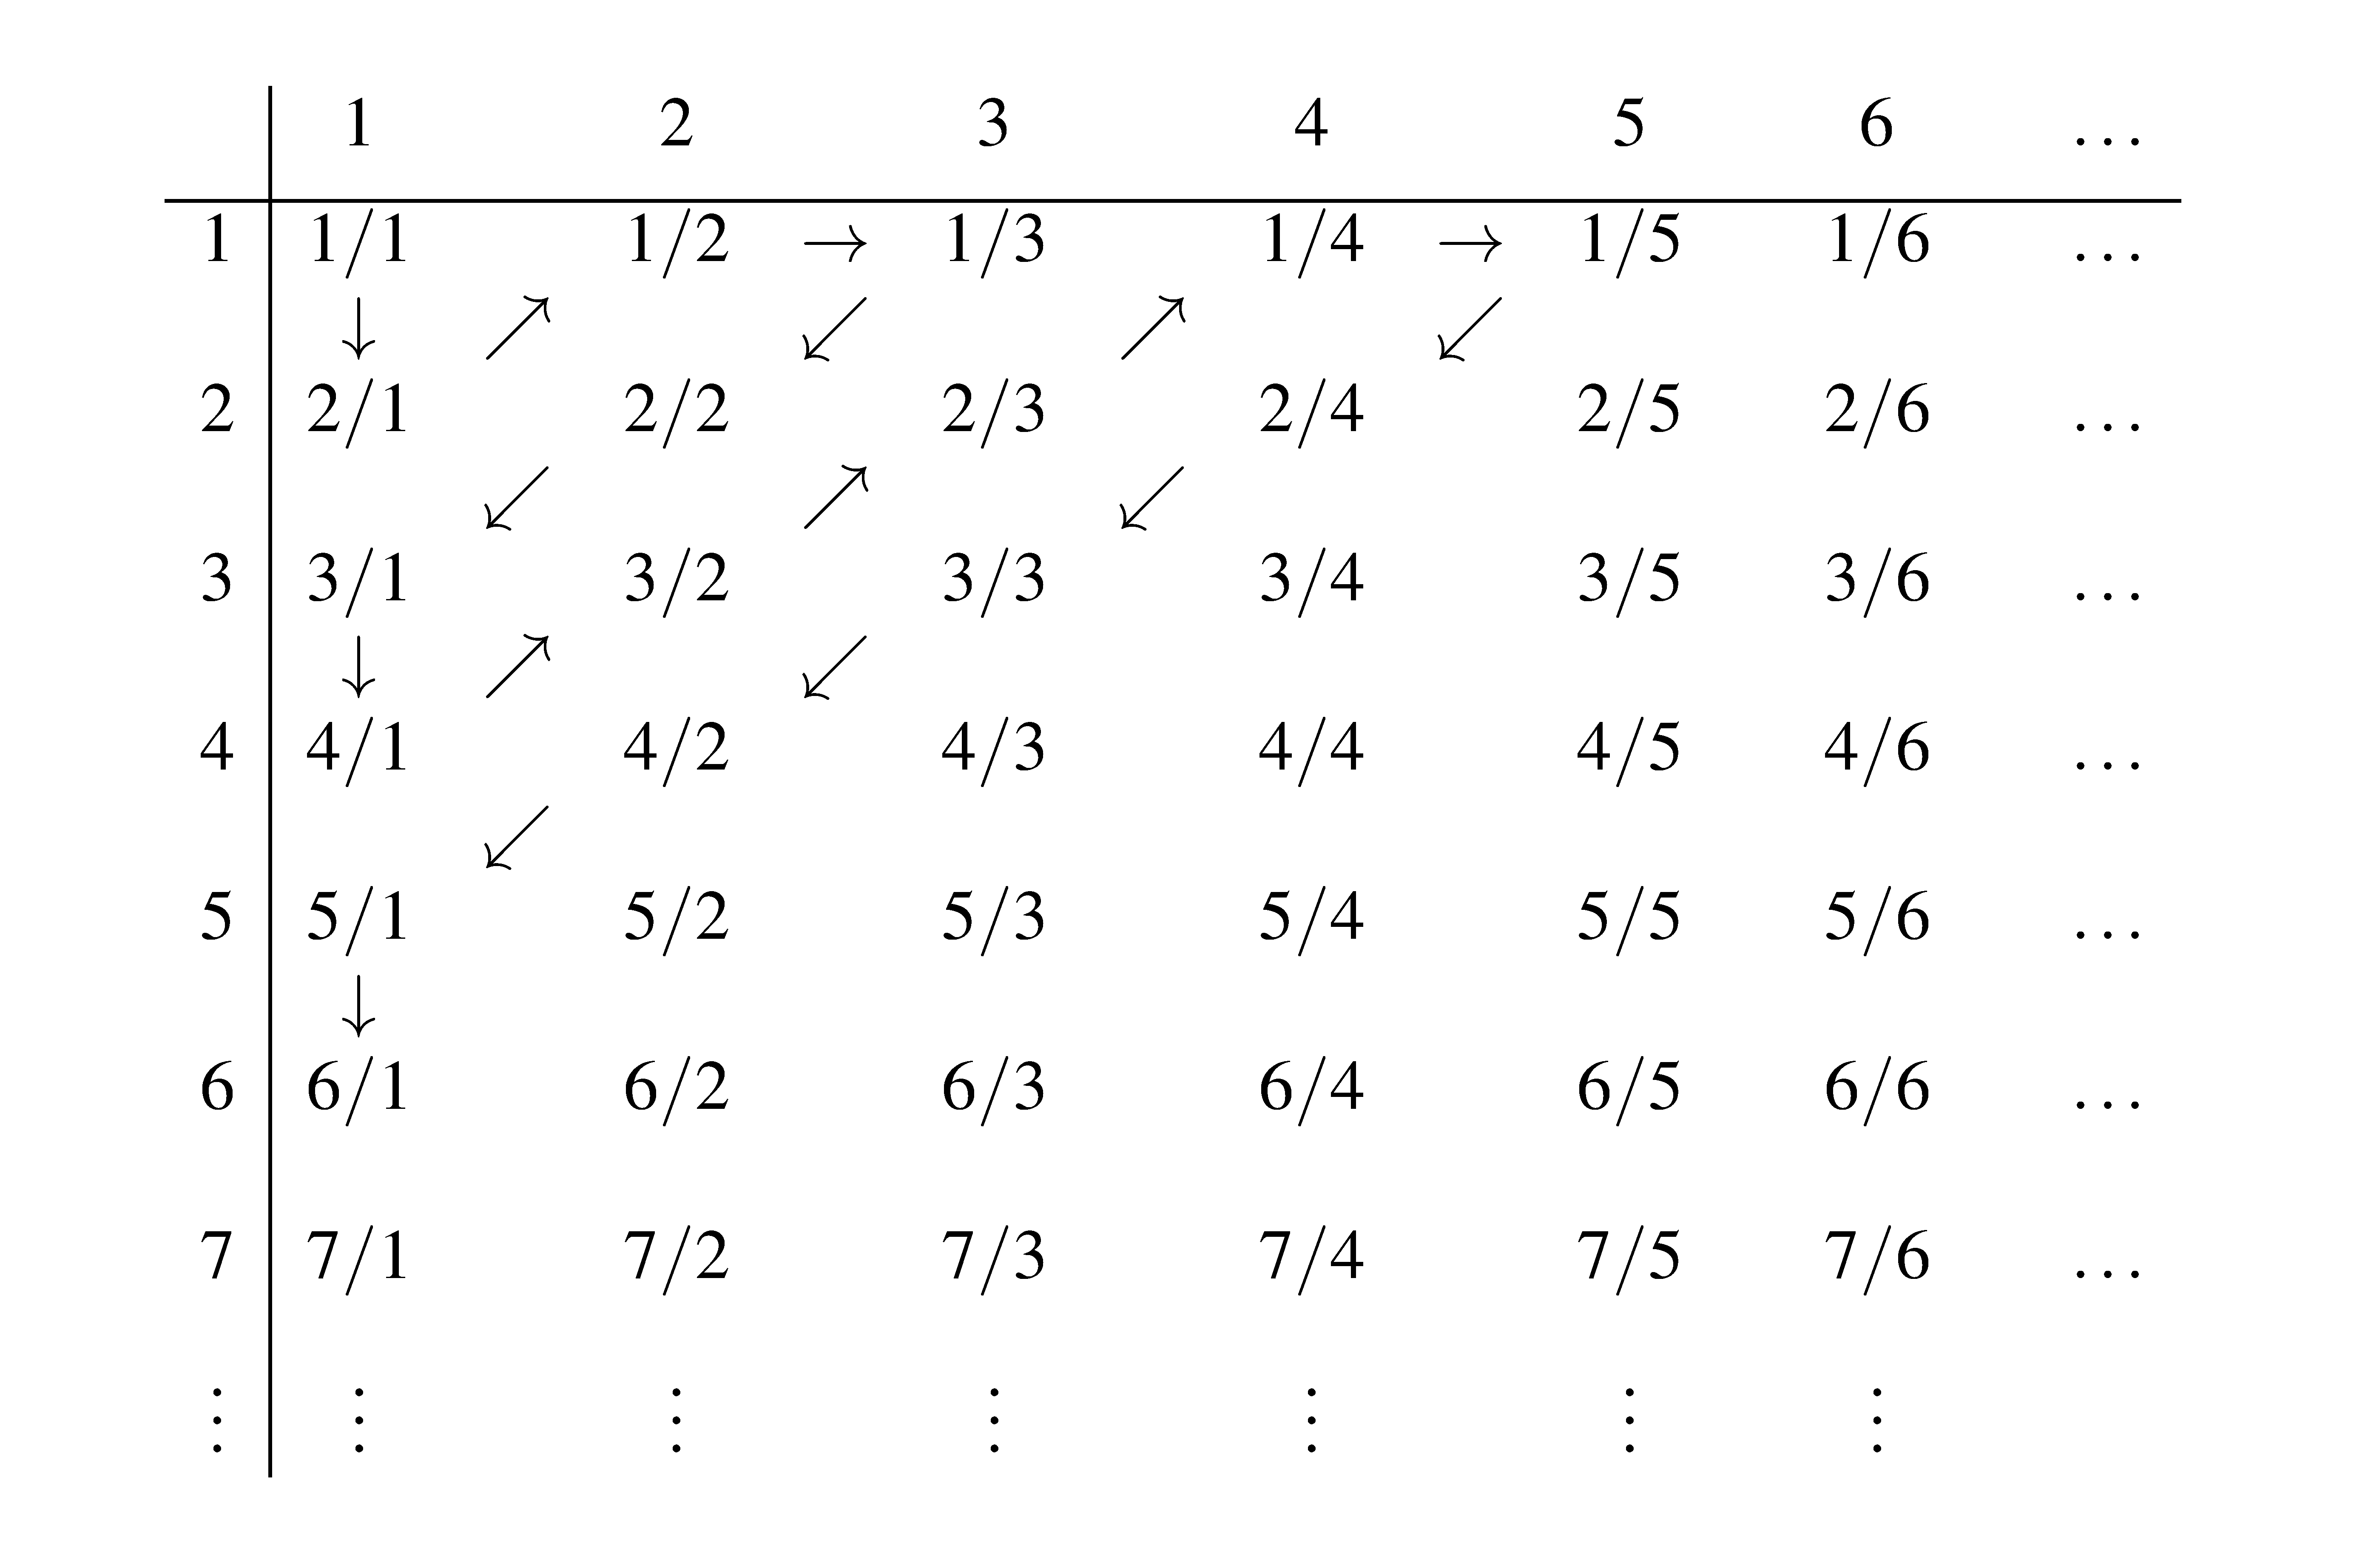
\includegraphics[width=0.8\textwidth]{sup/array}
  

\newcommand{\f}[2]{\small{#1/#2}} 

\newcommand{\ra}{\ensuremath{\rightarrow}} 

\newcommand{\da}{\ensuremath{\downarrow}} 

\newcommand{\nea}{\ensuremath{\nearrow}} 

\newcommand{\swa}{\ensuremath{\swarrow}}
\renewcommand{\arraystretch}{1}
\renewcommand{\tabcolsep}{3pt}

\begin{tabular}{ccccccccccccc}

 \rowcolor{lgray}
 \f{1}{1}	& 		&\f{1}{2}	&\ra  	&\f{1}{3}	& 		&\f{1}{4}	& \ra 	&\f{1}{5}	& 		&\f{1}{6} 	& 	&\ldots\\[0pt]

 \da		&\nea 	&        	&\swa &        		&\nea 	&        	&\swa 	&        	&	 	&        	& 	&	      \\[0pt]

 \rowcolor{lgray}
 \f{2}{1}& &\f{2}{2}& &\f{2}{3}& &\f{2}{4}& &\f{2}{5}& &\f{2}{6}& &\ldots\\[0pt]

		 &  \swa      & & \nea       & & \swa       & &        & &        & &      \\[0pt]

 
\rowcolor{lgray}
 \f{3}{1}& &\f{3}{2}& &\f{3}{3}& &\f{3}{4}& &\f{3}{5}& &\f{3}{6}& &\ldots\\[0pt]


 \da		&\nea &        &\swa &        & &        & &        & &        & &      
 \\[0pt]

 \rowcolor{lgray}
 \f{4}{1}& &\f{4}{2}& &\f{4}{3}& &\f{4}{4}& &\f{4}{5}& &\f{4}{6}& &\ldots\\[0pt]

				& \swa&        & &        & &        & &        & &        & &      \\[0pt]
 
 \rowcolor{lgray}
 \f{5}{1}& &\f{5}{2}& &\f{5}{3}& &\f{5}{4}& &\f{5}{5}& &\f{5}{6}& &\ldots\\[0pt]

				\da	& \nea &        & &        & &        & &        & &        
					& &      \\[0pt]

					
 \rowcolor{lgray}
 \f{6}{1}& &\f{6}{2}& &\f{6}{3}& &\f{6}{4}& &\f{6}{5}& &\f{6}{6}& &\ldots\\[0pt]

		 &        & &        & &        & &        & &        & &      \\[0pt]
 
 \rowcolor{lgray}
 \f{7}{1}& &\f{7}{2}& &\f{7}{3}& &\f{7}{4}& &\f{7}{5}& &\f{7}{6}	& &\ldots\\[0pt]

 
 \vdots &&\vdots  &&\vdots  &&\vdots  &&\vdots  &&\vdots  &&\\


\end{tabular}



\caption{Procedure for enumerating all positive fractions.}
\label{fig:fractions}
 \end{center}
\end{figure}

So fractions are countable: the first is \textfrac{1}{1}, the second is 
\textfrac{2}{1}, the third is \textfrac{1}{2}, etc.  One way of thinking about 
what we are doing is that we are assigning ID numbers to each fraction where 
each ID number is a natural number.  Even though one might feel that there are 
many more fractions than there are natural numbers, we can in fact give each and 
every fraction its own unique ID number without exhausting the pool of ID 
numbers.



\subsection{Countability of sentences}


Suppose \lL[] has infinitely many atomic sentences \p{A_1}, \p{A_2}, \p{A_3}, 
\ldots.  We want to enumerate all sentences of \lL{}. How could we do that? We 
will proceed in stages.

Let us first classify the sentences of \lL{}. We will call our atomic sentences 
class-0 sentences. Class-1 sentences are all class-0 sentences and all complex 
sentences that can be formed out of class-0 sentences by applying a single 
connective once. Class-3 sentences are all class-1 sentences and all complex 
sentences that can be formed out of class-1 sentences by applying a single 
connective once.  More generally:
\begin{description}
 \item[Class-0] sentences are atomic sentences.
 \item[Class-(n+1)] sentences are all class-n sentences plus all sentences that 
  can be formed out of at most two class-n sentences by applying a single 
  connective once.
\end{description}

Notice that any sentence of \lL{} must belong to some class-n (more precisely, 
there is an n such that the sentence belongs to any class-m such that m$\geq$n).
We will now show that for each n, class-n sentences are countable. 

Let's start with class-0 sentences. They are the atomic sentences of \lL{} and 
by the definition of formal languages, class-0 sentences must be countable. So 
class-0 sentences are countable.

What about class-1 sentences? Class-1 sentences are all class-0 sentences and 
all those sentences that can be formed out of class-0 sentences by applying a 
single connective once. Given this definition of class-1 sentences,  a class-1 
sentence must take one of the following forms:
\begin{itemize}
 \item \p{s}
 \item \p{\lnot s}
 \item \p{s\land t}
  \item \p{s\lor t}
 \item \p{s\limplies t}
\end{itemize}
where \p{s} and \p{t} are class-0---i.e., atomic---sentences. So if we have a 
way of walking through each and every pair of class-0 sentences and listing the 
five class-1 sentences that can be formed out of each pair, we have a way of 
enumerating all class-1 sentences. Here is a procedure that will do the job:

\begin{description}
 \item[Enumerating class-1 sentences]
Walk through  the list of fractions and do the following: given the fraction 
\textfrac{n}{m}, list \p{A_n}, \p{\lnot A_n}, \p{A_n\land A_m}, \p{A_n \lor A_m}, 
\p{A_n\limplies A_m} where any \p{A_i} is a class-0 sentence (i.e., an atomic 
sentence).
\end{description}

As we walk through the fractions, we will produce every class-0 sentence as well 
as any complex sentence that can be formed out of class-0 sentences by applying 
a single connective once. So this is a procedure for enumerating all class-1 
sentences in groups of five.

What about class-2 sentences? We can enumerate them, too:

\begin{description}
 \item[Enumerating class-2 sentences]
Walk through  the list of fractions and do the following: given the fraction 
\textfrac{n}{m}, list \p{S_n}, \p{\lnot S_n}, \p{S_n\land S_m}, \p{S_n \lor S_m}, 
\p{S_n\limplies S_m}, where \p{S_1}, \p{S_2}, \ldots are all the class-1 
sentences.
\end{description}

Since we know that class-1 sentences are countable, we know that there is a 
list of class-1 sentences \p{S_1}, \p{S_2}, \ldots that covers all class-1 
sentences and that therefore this procedure will enumerate all class-2 
sentences.  

We could continue in this vein but there are infinitely many classes. We need a 
better way. And there is. The way we enumerate class-1 and class-2 sentences 
shows that for any n we can enumerate class-(n+1) sentences in the following way:

\begin{description}
 \item[Enumerating class-(n+1) sentences]
Walk through  the list of fractions and do the following: given the fraction 
\textfrac{i}{j}, list \p{S_i}, \p{\lnot S_i}, \p{S_i\land S_j}, \p{S_i \lor S_j}, 
\p{S_i\limplies S_j}, where \p{S_1}, \p{S_2}, \ldots are sentences of class-n.
\end{description}

If the sentence of class-n are countable, this procedure will enumerate all 
class-(n+1) sentences. That is, if class-n sentences are countable, so are 
class-(n+1) sentences. We can now see that for any n, class-n sentences are 
countable: class-0 sentences are countable. So class-1 sentences are countable.  
So class-2 sentences are countable. So class-3 sentences are countable. Etc. 


But what about all the sentences of \lL{} taken together? That is, not just the 
sentences of a particular class-n, but all the infinitely many classes taken 
together.  Can we enumerate them? That's easy, too:

\begin{description}
 \item[Enumerating sentences of \lL{}] Walk through the list of fractions and do 
  the following: given the fraction \textfrac{n}{m}, list the m-th sentence of 
  class-n sentences.
\end{description}

For any sentence of \lL{}, it will eventually show up on the list of sentences 
generated in this way. Thus, the sentences of \lL{} are countable even when 
\lL{} has infinitely many atomic sentences. Put another way, you could assign a  
unique natural number as an ID to each and every sentence of \lL{} without 
worrying about exhausting the pool of ID numbers.


\subsection{Things to note about the argument}


Strictly speaking, we have shown more than that the sentences of \lL{} are 
countable. What we have shown is known as recursive enumerativity.  Roughly, 
that means it is possible to write a computer program to generate a list of all 
the sentences of \lL{}.  Not everything that is countable can be enumerated by a 
computer program. For instance, consider a list of all the winning numbers of a 
lottery.  That's countable, but if the lottery organizers know what they are 
doing, it is not possible to write a program that can generate the list of all 
winning numbers. The only way to list up all the winning numbers is by waiting 
for the drawings to take place (otherwise, you could get rich quick by writing a 
program that lists all the winning number, running it faster than the lottery 
numbers are drawn and buying the right tickets).  There is something special and 
interesting about the fact that the sentences of \lL{} are recursively 
enumerable.

The procedure we used for enumerating the sentences of \lL{}  will produce a 
highly redundant list because each class of sentences contains all members of 
the lower-numbered classes. If you don't like redundant lists, you can add the 
instruction `if the sentence has been listed previously, don't list it'.

There are infinitely many ways of enumerating the sentences of \lL{}.  Usually 
sentences are enumerated for a purpose and the method of enumeration used is 
tailored for the purpose.  The way we used here will be useful later for proving 
what is known as completeness of sentential logic               
(Section~\ref{sec:propCompleteness}).   A truly momentous result known as 
G\"odel's Incompleteness Theorem was proven using a different, very clever 
numbering scheme (That theorem concerns a formal language that is more complex 
than \lL{}.)

On a more prosaic level, computers represent sentences as  numbers (by assigning 
a number to each character and stringing them together).  That's a way of 
assigning a unique ID to each distinct sentence. That works, and we don't have 
to worry about running out of numbers to represent sentences. Some numbering 
schemes are easy to reverse in the sense that given an ID number it is 
relatively easy to figure out which sentence it belongs to. Some schemes are 
harder to reverse. Digital encryption works by using schemes that are especially 
difficult to reverse without some extra information (the extra information is 
often called the decryption key). 

What if \lL{} has only finitely many atomic sentences? In that case, each class 
of sentences has only finitely many sentences. But there still are infinitely 
many classes. You can use the same procedure for enumerating sentences of \lL{} 
by adding `if there is no m-th sentence of class-n, skip to the next fraction'.

Suppose there are 100 students and each gets a unique ID number. If we add more 
students to the mix, we will need to get hold of \emph{new} ID numbers to assign 
unique ID numbers to students in the enlarged group. Suppose there are 
infinitely many class-0 sentences. You can assign each sentence a unique ID so 
that each natural number is the ID of some sentence. That is, there are no 
numbers you can add to your pool of ID numbers.  And yet, if you add class-1 
sentences to the mix---there are infinitely many of them---you will be able to 
assign a unique ID to each and every sentence in that combined group of 
sentences by recycling the ID numbers you used for class-0 sentences.  And you 
can do this even if you add infinitely many classes each of which has infinitely 
many sentences. That's a bit mind-boggling. You might suspect that there can be 
no such thing as having so many things you genuinely cannot give them unique IDs, 
but a very simple argument can show that that's not so. Let me close this 
chapter with a discussion of that.



\section{Cantor's Diagonal Argument}\label{sec:diagonalization}

Consider the way we produced the list of interpretations earlier. If there is only one 
atomic sentence, there are two interpretations. As we add an atomic sentence, the number 
of interpretations doubles.  So if there are \p{N} sentences, there are $2^N$ interpretations.   
For instance, if there are 3 atomic sentences, there are $2^3=8$ interpretations.  If 
there are 8 atomic sentences, there are $2^8=256$ interpretations. And so on.  
How many interpretations are there if there  are infinitely many atomic 
sentences?  Well, infinitely many. But is the number of interpretations 
countable? The answer is No.  Here's an argument due to Georg \citet{Cantor1891} 
known as the Diagonal Argument.








Take the way we have been listing interpretations when constructing truth tables.  
Imagine a list of interpretations constructed in that way for infinitely many 
atomic sentences by repeating the procedure infintely many times. We know 
exactly what such a list looks like.  The first row has only T's. The second row 
starts with a single F and is followed by only T's.  The third row starts with a 
T followed by an F and then only T's. The fourth row starts with two F's and 
then only T's.  Etc.  Starting from top of the list, the whole thing will look 
like Figure \ref{fig:inf-tt-table}.


 \begin{center}

\begin{tabular}{cccccccc}

 & \footnotesize{\Circled[outer color=white]{T}}& \footnotesize{\Circled[outer 
color=white]{T}} & \footnotesize{\Circled[outer color=white]{T}} & 
\footnotesize{\Circled[outer color=white]{T}} & \footnotesize{\Circled[outer 
color=white]{T}} & \footnotesize{\Circled[outer color=white]{T}} & \ldots\\ 

 \rowcolor{lgray}
				  & \footnotesize{F} & \footnotesize{T} & \footnotesize{T} & 
 \footnotesize{T} & \footnotesize{T} & \footnotesize{T} & \ldots\\

				  & \footnotesize{T} & \footnotesize{F} & \footnotesize{T} & 
 \footnotesize{T} & \footnotesize{T} & \footnotesize{T} &  \ldots\\


 \rowcolor{lgray}
				  &  \footnotesize{F} & \footnotesize{F} & \footnotesize{T} & 
 \footnotesize{T} & \footnotesize{T} & \footnotesize{T} & \ldots\\

								& \footnotesize{T} & \footnotesize{T} & 
 \footnotesize{F} & \footnotesize{T} & \footnotesize{T} & \footnotesize{T} & 
 \ldots\\


 \rowcolor{lgray}
				  & \footnotesize{F} & \footnotesize{T} & \footnotesize{F} & 
 \footnotesize{T} & \footnotesize{T} & \footnotesize{T} & \ldots\\

				  & \vdots   &\vdots    & \vdots   & \vdots   & \vdots   & 
 \vdots   & \\
\end{tabular}
 \captionof{figure}{interpretations for infinitely many atomic sentences}             
 \label{fig:inf-tt-table}
 \end{center}



It may seem that the table must list all the interpretations. After all, we know exactly 
how to proceed as we increase the number of atomic sentences one by one. At no 
point will the procedure miss an interpretation, so how could the procedure miss 
an interpretation when extending it to infinitely many atomic sentences? And if 
the list of interpretations is complete, clearly the interpretations are 
countable: the first is on the first row, the second is on the second row, etc. 

Matters, however, are not this simple. It is easy to construct an interpretation 
that is not on the list. Here is how. An interpretation can be treated as a just 
a string of T's and F's. Let's construct new interpretation \p{\mathcal N}  in 
the following way:

\begin{itemize}
 \item If the first letter of the first interpretation is a T, the first letter of 
  \p{\mathcal N} is F. If the first letter of the first interpretation is an F, the first 
  letter of \p{\mathcal N} is a T.

 \item If the second letter of the second interpretation is a T, the second letter of 
  \p{\mathcal N} is F. If the second letter of the second interpretation is an F, the 
  second letter of \p{\mathcal N} is a T.

 \item More generally, the n-th letter of \p{\mathcal N} is a T iff. the n-th 
  letter of the n-th interpretation is an F. 

\end{itemize}

The following illustrates the method:
\begin{center}

\begin{tabular}{cccccccc}
 & \footnotesize{\textcircled{T}}& \footnotesize{T} & \footnotesize{T} & 
 \footnotesize{T} & \footnotesize{T} & \footnotesize{T} & \ldots\\ 

 \rowcolor{lgray}
				  & \footnotesize{F} & \footnotesize{\textcircled{T}} & 
 \footnotesize{T} & \footnotesize{T} & \footnotesize{T} & \footnotesize{T} & 
 \ldots\\

				  & \footnotesize{T} & \footnotesize{F} & 
 \footnotesize{\textcircled{T}} & \footnotesize{T} & \footnotesize{T} & 
 \footnotesize{T} &  \ldots\\


 \rowcolor{lgray}
				  &  \footnotesize{F} & \footnotesize{F} & \footnotesize{T} & 
 \footnotesize{\textcircled{T}} & \footnotesize{T} & \footnotesize{T} & \ldots\\

								& \footnotesize{T} & \footnotesize{T} & 
 \footnotesize{F} & \footnotesize{T} & \footnotesize{\textcircled{T}} & 
 \footnotesize{T} & \ldots\\


 \rowcolor{lgray}
				  & \footnotesize{F} & \footnotesize{T} & \footnotesize{F} & 
 \footnotesize{T} & \footnotesize{T} & \footnotesize{\textcircled{T}} & \ldots\\

				  & \vdots   &\vdots    & \vdots   & \vdots   & \vdots   & 
 \vdots   & \\

\hline
 \footnotesize{$\mathcal N$:}	  & \footnotesize{F} & \footnotesize{F} & 
 \footnotesize{F} & \footnotesize{F} & \footnotesize{F} & \footnotesize{F} & 
 \ldots\\

\end{tabular}
\captionof{figure}{Diagonalization}
\end{center}

It shows the top left corner of our list of interpretations. Each row above the 
horizontal line is an infinitely long interpretation.  We construct the 
interpretation \p{\mathcal N} below the horizontal line by taking each circled 
letter and `flipping' it (T to F, F to   T).  \p{\mathcal N} differs from the 
first interpretation because of the first letter, from the second interpretation 
because of the second letter, from the third interpretation because of the third 
letter, etc. \p{\mathcal N} differs from each and every  interpretation on the 
list. That means that \p{\mathcal N} is not on the list.  Thus, the list of 
interpretation is not a complete list.  I hope you can see why the argument is 
called the \emph{Diagonal} Argument. 

The interpretation \p{\mathcal N} we have found is the one  that assigns \emph{F} 
to all atomic sentences. And that cannot be on the list since given the way we 
construct the list of interpretations, that particular interpretation must be 
the last one. But an infinite list cannot have a last line: that's what it is to 
be \emph{infinte}---without end. 

You might think we can handle that problem by simply adding the interpretation we have 
found to the list. Like this:

 \begin{center}

\begin{tabular}{ccccccccc}

	  & \footnotesize{\Circled[outer color=white]{F}} & 
 \footnotesize{\Circled[outer color=white]{F}} & \footnotesize{\Circled[outer 
 color=white]{F}} & \footnotesize{\Circled[outer color=white]{F}} & 
 \footnotesize{\Circled[outer color=white]{F}} & \footnotesize{\Circled[outer 
 color=white]{F}} & \footnotesize{\Circled[outer color=white]{F}}& \ldots\\
 
 \rowcolor{lgray}
				  & \footnotesize{T}& \footnotesize{T} & \footnotesize{T} & 
 \footnotesize{T} & \footnotesize{T} & \footnotesize{T} & \footnotesize{T}  & 
 \ldots\\ 

				  & \footnotesize{F} & \footnotesize{T} & \footnotesize{T} & 
 \footnotesize{T} & \footnotesize{T} & \footnotesize{T} &\footnotesize{T}   
				  &\ldots\\

 \rowcolor{lgray}
				  & \footnotesize{T} & \footnotesize{F} & \footnotesize{T} & 
 \footnotesize{T} & \footnotesize{T} & \footnotesize{T} &\footnotesize{T}    
				  &\ldots\\


				  &  \footnotesize{F} & \footnotesize{F} & \footnotesize{T} & 
 \footnotesize{T} & \footnotesize{T} & \footnotesize{T} &\footnotesize{T}   
				  &\ldots\\

 \rowcolor{lgray}
								& \footnotesize{T} & \footnotesize{T} & 
 \footnotesize{F} & \footnotesize{T} & \footnotesize{T} & \footnotesize{T} 
				  &\footnotesize{T}  & \ldots\\


				  & \footnotesize{F} & \footnotesize{T} & \footnotesize{F} & 
 \footnotesize{T} & \footnotesize{T} & \footnotesize{T} &\footnotesize{T} & 
 \ldots\\

				  & \vdots   &\vdots    & \vdots   & \vdots   & \vdots   & 
 \vdots   & \vdots &  \\
\end{tabular}
\captionof{figure}{list of interpretations with missing interpretation added}             
\end{center}

But this won't do. We can construct a interpretation that is not on this list: 

\begin{center}
\begin{tabular}{ccccccccc}

	  & \footnotesize{\textcircled{F}} & \footnotesize{F} & \footnotesize{F} & 
 \footnotesize{F} & \footnotesize{F} & \footnotesize{F} & \footnotesize{F} 
				  &\ldots\\
 
 \rowcolor{lgray}
				  
				  & \footnotesize{T}& \footnotesize{\textcircled{T}} & 
 \footnotesize{T} & \footnotesize{T} & \footnotesize{T} & \footnotesize{T} & 
 \footnotesize{T} & \ldots\\
				  
				  & \footnotesize{F} & \footnotesize{T} & 
 \footnotesize{\textcircled{T}} & \footnotesize{T} & \footnotesize{T} & 
 \footnotesize{T} & \footnotesize{T} & \ldots\\

 \rowcolor{lgray}
				  & \footnotesize{T} & \footnotesize{F} & \footnotesize{T} & 
 \footnotesize{\textcircled{T}} & \footnotesize{T} & \footnotesize{T} &  
 \footnotesize{T} & \ldots\\


				  &  \footnotesize{F} & \footnotesize{F} & \footnotesize{T} & 
 \footnotesize{T} & \footnotesize{\textcircled{T}} & \footnotesize{T} & 
 \footnotesize{T} & \ldots\\

 \rowcolor{lgray}
								& \footnotesize{T} & \footnotesize{T} & 
 \footnotesize{F} & \footnotesize{T} & \footnotesize{T} & 
 \footnotesize{\textcircled{T}} &\footnotesize{T} &  \ldots\\


				  & \footnotesize{F} & \footnotesize{T} & \footnotesize{F} & 
 \footnotesize{T} & \footnotesize{T} & \footnotesize{T} & 
 \footnotesize{\textcircled{T}} & \ldots\\

				  & \vdots   &\vdots    & \vdots   & \vdots   & \vdots   & 
 \vdots   & \vdots   &\\
\hline
 \footnotesize{$\mathcal N$:}	  & \footnotesize{T} & \footnotesize{F} & 
 \footnotesize{F} & \footnotesize{F} & \footnotesize{F} & \footnotesize{F} & 
 \footnotesize{F} &
 \ldots\\
\end{tabular}
\captionof{figure}{Finding another missing interpretation}

\end{center}


The point is completely general. It is not just that our particular way of 
generating the list of interpretations fails when dealing with infinitely many 
atomic sentences. Given any list of interpretations for infinitely many atomic 
sentences, we can find an interpretation that is not on the list.  Here is an 
illustration to see that:

\begin{center}

\begin{tabular}{cccccccc}

 & \textcircled{\footnotesize{T}} & \footnotesize{F} & \footnotesize{T} & 
 \footnotesize{T} & \footnotesize{F} & \footnotesize{T} & \ldots\\ 

 \rowcolor{lgray}
				  & \footnotesize{F} & \textcircled{\footnotesize{T}} & 
 \footnotesize{F} & \footnotesize{F} & \footnotesize{T} & \footnotesize{T} & 
 \ldots\\

				  & \footnotesize{T} & \footnotesize{T} & 
 \textcircled{\footnotesize{F}} & \footnotesize{T} & \footnotesize{T} & 
 \footnotesize{T} &  \ldots\\


 \rowcolor{lgray}
				  &  \footnotesize{F} & \footnotesize{F} & \footnotesize{F} & 
 \textcircled{\footnotesize{T}} & \footnotesize{F} & \footnotesize{T} & \ldots\\

								& \footnotesize{F} & \footnotesize{F} & 
 \footnotesize{F} & \footnotesize{T} & \textcircled{\footnotesize{F}} & 
 \footnotesize{F} & \ldots\\


 \rowcolor{lgray}
				  & \footnotesize{T} & \footnotesize{T} & \footnotesize{T} & 
 \footnotesize{T} & \footnotesize{F} & \textcircled{\footnotesize{T}} & \ldots\\

				  & \vdots   &\vdots    & \vdots   & \vdots   & \vdots   & 
 \vdots   & \\
\hline
 \footnotesize{$\mathcal N$:}	  & \footnotesize{F} & \footnotesize{F} & 
 \footnotesize{T} & \footnotesize{F} & \footnotesize{T} & \footnotesize{F} & 
 \ldots\\
\end{tabular}

\end{center}

That means, the very idea of a complete list of interpretations when dealing with 
infinitely many atomic sentence is incoherent.  That is what the Diagonal 
Argument shows.  Given infinitely many atomic sentences, there are more interpretations 
than there are natural numbers.  We say that the set of interpretations has higher 
\emph{cardinality} than the natural numbers.

We now know that there really are more interpretations than there are atomic 
sentences---that's even true if the number of atomic sentences is infinite as we 
have just shown. What about the number of truth conditions? 

A truth condition of a sentence  specifies for each interpretation whether or not the 
sentence is true in that interpretation.  That means that if \p{\mathtt{m}} is the 
number of interpretations, the number of possible truth conditions is \p{2^\mathtt{m}}.  
For instance, if there are 8 atomic sentences, there are 256 interpretations  and $2^{256}
\approx 1.1\times 10^{77}$ possible truth conditions.  For comparison, our 
planet Earth is estimated to contain about $10^{50}$ atoms.\footnote{\url{https:
//www.fnal.gov/pub/science/inquiring/questions/atoms.html}}
With just one more atomic sentence---9 of them---there are about $2^{512}\approx 
1.3\times 10^{154}$ possible truth conditions for a sentence. That vastly---and 
that's putting it very mildly---exceeds the estimated number of atoms in the 
observable universe which is around $10^{80}$ atoms.\footnote{\url{https:
//en.wikipedia.org/wiki/Observable_universe}} This gives you a glimpse of the 
expressive capacities of natural languages: they can surely say more than what 
we can with just 9 atomic sentences in \lL{}. 

These considerations show that the number of truth conditions is larger than the 
number of interpretations in case the number of atomic sentences is finite.  And we can 
prove that this is so even if there are infinitely many atomic sentences.

The proof proceeds via a slight reformulation of the Diagonal Argument.  Notice 
that the question whether or not there are countably many interpretations is the 
same as the question whether or not  it is possible to pair atomic sentences 
with interpretations without residue on either side. An interpretation can be 
understood as a subset of atomic sentences: each interpretation contains those 
atomic sentences that are true in that interpretation. So the question is 
whether or not the set of atomic sentences can be paired, without residue on 
either side,  with sets of atomic sentences---these latter are the subsets of 
the set of atomic sentences.  Take any set \p{\mathcal S} and consider a pairing 
of its members with subsets of \p{\mathcal S}. Could such a pairing be 
one-to-one without residue? The answer is no.  We can construct a  new subset 
\p{\mathcal N} in the following way: for any member \p{e} of \p{\mathcal S}, 
\p{e} is in \p{\mathcal N} iff.  \p{e} is not in the subset of \p{\mathcal S} 
paired with it.  \p{\mathcal N} is not paired with any member of \p{\mathcal S} 
since for any member \p{e} of \p{\mathcal S}, \p{\mathcal N} differs from the 
subset of \p{\mathcal S} paired with \p{e}. This shows that the cardinality of 
the set of all the subsets of \p{\mathcal S}---a.k.a. the \emph{power set} of 
\p{\mathcal S}---must be larger than the cardinality of \p{\mathcal S}.  This is 
known as Cantor's Theorem. 

The argument just given can be given for any set and its power set: thus, as we 
have already seen, the set of interpretations has higher cardinality than the 
set of all atomic sentences. Now, a truth condition is a set of interpretations: 
the set of all the interpretations in which a sentence is true.  So the 
cardinality of truth conditions is higher than the cardinality of 
interpretations. And the set of all the subsets of truth conditions has even 
higher cardinality, and so on.   This opens up a realm of mathematical entities 
that David Hilbert called Cantor's paradise  \citeyearpar{hilbert1926}.






\chapter{Proofs: Natural Sequent Calculus}\label{ch:SequentCalculus}


\section{Arguments}\label{sec:derivation intro 2}

In the previous chapter we defined a formal language. Consider native speakers 
of such a formal language \lL{}. They can say many things: not just the atomic 
sentences, but an infinite variety of compound sentences using the logical 
connectives \p{\lnot}, \p{\land}, \p{\lor}, and \p{\limplies}. Not only are they 
capable of formulating an infinite variety of sentences, they are also capable 
of saying sentences with a large variety of different truth conditions, i.e., 
meanings.  Just how large that variety is depends on the number of atomic 
sentences, of course. 

But we do more than just say things using language. One very important use of 
language is the presentation of \emph{arguments}. Consider:

\begin{Example}\label{ex:econo-1}

More investment [in indoor ventilation] would be money well spent. Better indoor 
air boosts academic performance---maths and reading scores go up. Office-workers 
benefit, too. Researchers have found the cognitive scores of people in 
well-ventilated offices are 61\% higher than those of workers in conventional 
office set-ups. (from \emph{The Economist},  May 29, 2021)

\end{Example}

This little snippet consists of four sentences. But it is not simply an 
enumeration of four facts. Rather, it is trying to persuade the reader that 
investment in indoor ventilation would be money well spent. And it attempts that 
not by bluntly asserting the claim but by providing reasons in support of the 
claim that investing in indoor ventilation makes sense. In short, it is an 
argument. 

The claim that an argument is meant to support is called the \emph{conclusion}.  
A claim adduced in support of the conclusion is called a \emph{premise}.  
Arguments often have multiple premises. In the above example, the conclusion is 
that investment in indoor ventilation is money well spent. And there are two 
stated premises: (a) better indoor air boosts academic performance; and (b)
 researchers have found the cognitive scores of people in well-ventilated 
 offices are 61\% higher than those of workers in conventional office set-ups.

Our main topic of interest in this chapter is arguments. We will be looking at 
highly formalized arguments, but before doing that let me discuss natural 
language arguments a bit more. It will help understanding the virtues of the 
formalizations we will be studying.

Consider:

\begin{Example}\label{ex:econo-2}


From April, British prisons will have to screen all inmates who have experienced 
domestic violence for brain injuries. Such screening should be extended to all 
prisoners. It would enable staff to identify those whose brains have been 
damaged and offer them appropriate support. (from \emph{The Economist}, March  
27, 2021)

\end{Example}


The conclusion of this argument is clear enough: all prisoners should be 
screened for brain injuries. But how is that conclusion supported? Apart from 
the conclusion, the snippet states two facts:

\begin{itemize}
 \item[(a)] From April British prisons have to screen all inmates who have 
  experienced domestic violence for brain injuries.
 \item[(b)] Screening for brain injuries enables staff to identify those whose 
  brains have been damaged and offer them appropriate support.
\end{itemize}

Does (a) support the conclusion? Upon a little reflection, it seems not: even if 
British prisons did not screen any inmates, that would not weaken the case for 
screening them for brain injuries. So (a) is in fact not a premise. So the 
argument as stated has only one premise: (b). But does (b) support the 
conclusion?  Taking (b) to support the conclusion requires accepting that even 
criminals deserve support for dealing with the effects of brain injuries. You 
may find that obvious, but others find that highly controversial. The point: the 
snippet above contains a claim that is no part of the argument, and the argument 
depends on an unstated premise about what criminals deserve. And, if you think 
about it, the first example (Example~\ref{ex:econo-1}) also makes some unstated 
assumptions about what is worthy of spending money on. This is a common feature 
of arguments stated in natural languages.  We need to be careful to make sure we 
do not miss hidden premises, and be careful not to mistake some extraneous 
information as part of the argument.


\section{Diagrammatic Representations of Arguments in Tree Form}
\label{sec:argument tree}

An argument presents certain connections among thoughts. In particular, they 
present how some thoughts support other thoughts. You probably are familiar with 
things like mind maps as ways of presenting connections between ideas.  
Arguments can be presented in a similar fashion as diagrams.  For instance, 
Consider a simplified version of the argument in Example~\ref{ex:econo-1}:

\begin{Example}\label{ex:econo-1-simple}

More investment [in indoor ventilation] would be money well spent. Better indoor 
air boosts academic performance.

\end{Example}

We can represent this in the following way:

\vskip 1em

\begin{center}
\begin{forest}{for tree = {grow=north,s sep=1cm, edge = <-}}
 [More investment in indoor ventilation is money well spent.
 [Better indoor ventilation\\ boosts academic performance., align=center]
 ]
\end{forest}
\end{center}

\vskip 1em

The arrow represents the direction of support, so the idea expressed at the top 
of the diagram supports the idea expressed at the bottom. But, as already 
pointed out, it seems that there is another thought that is playing a role in 
supporting the conclusion. We can capture that:

\vskip 1em

\begin{center}
\begin{forest}{for tree = {grow=north,s sep=1cm, edge = <-}}
 [More investment in indoor ventilation is money well spent.
 [If better indoor ventilation\\ boosts academic performance{,}\\ then more 
 investment in indoor\\ ventilation is money well spent., align=center]
 [Better indoor ventilation\\ boosts academic performance., align=center]
 ]
\end{forest}
\end{center}

\vskip 1em

It is the two thoughts at the top taken together that support the conclusion at 
the bottom. The above is a very common pattern of argument known as \emph{modus 
ponens}.  We can make the pattern clear by replacing the sentences with letters.  
Let \p{A} stand for \pp{Better indoor ventilation boosts academic performance} 
and let \p{B} stand for \pp{more investment is money well spent}. Then the above 
can be represented as:


\begin{center}
\begin{forest}{for tree = {grow=north, s sep=1cm, edge=<-}}
  [\p{B}
  [if \p{A}{,} then \p{B}]
  [\p{A}]
  ]
 \end{forest}
 \captionof{figure}{Modus Ponens}
\end{center}

The sentences at the top are the premises, the sentence at the bottom the 
conclusion. If you think about the meaning of the conditional, it is clear that 
if the two premises are true, the conclusion must be, too. So the premises do 
provide good support for the conclusion, and it does not matter what \p{A} and 
\p{B} stand for.

We can also have more complex arguments. For instance, if you are asked why we 
should accept that better indoor ventilation boosts academic performance, we 
might answer that test scores go up when ventilation is improved, and that if 
scores go up, then that shows that better indoor ventilation boosts academic 
performance. We could represent the augmented argument  by the following diagram 
which has modus ponens occurring twice---once to get to \p{A}, and then to get 
to \p{B}: 

\vskip 1em
\begin{center}
 
 \begin{forest}{for tree = {grow=north, s sep=1cm, edge=<-}}
  [\p{B}
  [if \p{A}{,} then \p{B}]
  [\p{A}
  [if \p{C}{,} then \p{A}]
  [\p{C}]
  ]
  ]
 \end{forest}
 \captionof{figure}{Complex Argument}
\end{center}
\vskip 1em

More complicated arguments will be represented by larger diagrams. Arguments 
might be thought of as having structures akin to river systems: smaller streams 
flow together to form ever larger systems until they reach the conclusion.  
Investigating various structures of arguments reveals a few very common patterns 
of `confluences'. The above patterns which combines a conditional and the 
antecedent of the conditional is among the most common patterns.  Let me discuss 
some more common patterns.

Consider the following piece of reasoning:

\begin{Example}\label{ex:fed}

 The Central Bank will stop raising interest rates only if inflation has been 
 brought under control. But inflation has not been brought under control. So the 
 Central Bank will not stop raising interest rates.

\end{Example}

This has the following structure known as \emph{modus tollens} (recall that 
\pp{if A, then P} is another way of saying \pp{A only if B}):

\vskip 1em
\begin{center}
 \begin{forest}{for tree = {grow=north, s sep=1cm}}
  [not \p{A}
  [not \p{B}]
  [if \p{A}{,} then \p{B}]
  ]
 \end{forest}
 \captionof{figure}{Modus Tollens}
\end{center}
\vskip 1em

We omit the arrow heads: in such argument diagrams, the support is always from 
top to bottom.

Here is an example of another common pattern.  Socrates---often regarded as the 
founder of Western philosophy---argued that death is a good thing in the 
following way: death is one of two things; either it is like an eternal deep 
sleep which is a good thing; or death means moving to another world where you 
can spend an eternity talking to such interesting people like Homer and the 
ancient Greek heroes, which is a good thing; so either way death is a good thing; 
thus, death is a good thing.

This is known as an \emph{argument by cases}. Here is a way of representing this:

\vskip 1em
\begin{center}
 \begin{forest}{for tree = {grow=north, s sep=1cm}}
  [\p{C}
  [if \p{B}{,} then \p{C}]
  [if \p{A}{,} then \p{C}]
  [\p{A} or \p{B}]
  ]
\end{forest}
\captionof{figure}{Argument By Cases}
\end{center}
\vskip 1em

Here we have a confluence of three claims.

Here is one more example of a common pattern. Consider a well-known argument 
that you cannot go back in time and kill your biological mother before you were 
even conceived:

\begin{Example}

You plan to go back in time and kill your mother before you were even conceived.  
Suppose your plan succeeds. In that case, your mother does not conceive you, and 
you do not exist. On the other hand, for your plan to succeed, you must execute 
the plan, and that requires you to exist.  So if your plan succeeds, you do and 
do not exist, which is a contradiction. Thus, your plan cannot succeed.

\end{Example}

This is an instance of what is known as \emph{reductio ad absurdum} or argument 
by contradiction. This pattern can be represented as:

\vskip 1em
\begin{center}
 \begin{forest}{for tree = {grow=north, s sep=1cm}}
  [not \p{A}
  [if \p{A}{,} then not \p{B}]
  [if \p{A}{,} then \p{B}]
  ]
\end{forest}
\captionof{figure}{Reductio ad Absurdum}
\end{center}
\vskip 1em



\section{Arguments in Standard Form}\label{sec:standardForm}

Diagrammatic representations of arguments can be very helpful for understanding 
the structure of larger arguments, but they take a lot of space and are 
difficult to produce without the help of technology. A far more common way of 
representing an argument is in the form of a list of sentences. A simple list of 
sentences is a one-dimensional structure and cannot give us all the information 
that the two-dimensional diagrams in the previous section can represent. To make 
up for this shortcoming, we will add \emph{annotations} to each line that gives 
us extra information about how the sentences connect. For instance, Modus Ponens 
is represented as:

\begin{argument*}

 \aitem If A, then B\texpl{premise}
 
 \aitem A\texpl{premise}

 \aitem B\texpl{1,2, MP}

\end{argument*}

The annotations at the end of each line give us enough information to 
reconstruct the diagrams of the previous section. The keyword `premise' in the 
annotations of lines 1 and 2 tells us that they are not represented as supported 
by further nodes up the diagram. The `1,2' in the annotation of line 3 tells us 
that the sentence on line 3 is supported by the sentences on lines 1 and 2.  And 
this is enough to enable us to reconstruct the argument tree: 

\begin{center}
\begin{forest}{for tree = {grow=north, s sep=1cm}}
  [\p{B}
  [\p{A}]
  [if \p{A}{,} then \p{B}]
  ]
 \end{forest}
 \captionof{figure}{Modus Ponens}
\end{center}

The `MP'  in the annotation of line 3. names the pattern Modus Ponens.  As you 
can see, we only need the references to the supporting lines in the annotation 
to reconstruct the argument diagram, but it helps to explicitly name the pattern 
as it helps with checking whether the conclusion really is supported by the 
premises.

From here on, the normal way of presenting arguments will be in such list form.  
While I will occasionally display an argument in tree form when it helps making 
the structure of an argument more vivid, you do not have to produce such 
diagrams yourself. 

Apart from making sure that the list contains enough information to reconstruct 
the tree, we also require that an argument in \emph{standardized form}  be such 
that a given line cannot be supported by lines below it. So the direction of 
support is strictly from top to bottom. That helps with comprehension of the 
argument presented. 

When an argument is such that the conclusion cannot fail to be true if all the 
premises are true, it is said to be \emph{valid}. One of the important tasks of 
logic is figuring out which argument patterns are valid. 

Let me go through the patterns of arguments discussed in the previous section.  
They are all known to be valid. You can check that they are valid  by checking  
truth tables: could all the premises be true without the conclusion being true?


\subsection{Modus Ponens (MP)}

I already have shown how an instance of the use of modus ponens works:

\begin{argument*}

 \aitem If A, then B\texpl{premise}
 
 \aitem A\texpl{premise}

 \aitem B\texpl{1,2, MP}

\end{argument*}

Any argument with a premise P and conclusion C can be turned into a logically 
valid argument by adding the premise \pp{if P, then C}. For instance, suppose 
someone reasons, ``Donald is rich; therefore, he is fit to be the president of a 
country.'' We can turn this into a logically valid argument as follows:

\begin{argumentNamed*}[Argument 1]
\aitem If Donald is rich, then Donald is fit to be the president of a 
country.~~~\texpl{premise}

\aitem Donald is rich. \texpl{premise}

\aitem Donald is fit to be the president of a country. \texpl{1,2, MP}

\end{argumentNamed*}

While this is a valid argument---\emph{if} both premises are true, then the 
conclusion is also true---this need not give us a particularly strong reason to 
accept the conclusion: putting it cautiously, some people might think that 
recent history decisively shows that the first premise is false. A benefit of 
presenting arguments in standardized form is that it enables us to see what all 
the needed premises are which in turn allows us to see which premises might be 
suspect.

\subsection{Modus Tollens (MT)}

Here is Modus Tollens in standard form:

\begin{argument*}

 \aitem If A, then B. \texpl{premise}

 \aitem Not B.\texpl{premise}

 \aitem Not A. \texpl{1,2, MT}

\end{argument*}

Here is an example using \ref{ex:fed}:

\begin{argumentNamed*}[Argument 2]

 \aitem If the Central Bank will stop raising interests rates, then inflation 
 has been brought under control.\texpl{premise}
 
 \aitem Inflation has not been brought under control.\texpl{premise}

\aitem The Central Bank will not stop raising interest rates.  \texpl{1,
 2, MT}

\end{argumentNamed*}

\subsection{Argument By Cases (AC)}

Here is the argument by cases in standard form:

\begin{argument*}

 \aitem A or B\texpl{premise}
 
 \aitem If A, then C\texpl{premise}

 \aitem If B, then C\texpl{premise}

 \aitem C\texpl{1,2,3, AC}

\end{argument*}

If all premises are true, then at least one of A and B is true (by premise 1).  
If A is true, then C is true (premise 2). If B is true, then C is true (premise 
3). So C is true given all three premises are true. Thus, this argument form is 
valid. 

Of course, just because such an argument is valid does not mean that the 
argument is a good one. For instance, you might wonder whether Socrates is right 
that death must be one of the two things he lists; and even he is right about 
that, is it so obvious that death would be a good thing on both options---a day 
talking to Homer might be super interesting, but a whole eternity talking to him? 

\subsection{Reductio ad Absurdum (RAA)}

Here is Reductio ad Absurdum:

\begin{argument*}

 \aitem If A, then B \texpl{premise}

 \aitem If A, then not B \texpl{premise}

 \aitem Not A\texpl{1,2, RAA}

\end{argument*}

In the example about time travel we discussed earlier, let A be `your plan 
succeeds' and B be `you exist' which gives us:

\begin{argumentNamed*}[Argument 3]

 \aitem If your plan succeeds, then you exist.\texpl{premise}

 \aitem If your plan succeeds, then you are do not exist.\texpl{premise}

 \aitem Your plan does not succeed.\texpl{1,2, RAA}

\end{argumentNamed*}


\subsection{Extracting arguments from natural language texts}

Extracting arguments from natural language texts and putting them in 
standardized form takes some practice. Let me start with an example that 
illustrate some of the tricky aspects.

Julius Caesar was assassinated by a group of Roman senators led by Brutus. The 
conspirators accused Caesar of harboring ambitions of becoming the king of Rome 
(Rome was a republic at the time). In Shakespeare's fictionalized version of the 
events in the play \emph{Julius Caesar}, Marc Antony---a prominent prot\'eg\'e 
of Caesar---gives a speech at Caesar's funeral that turns the crowd against 
Brutus.  Here is a snippet from that speech:

\begin{quote}
You all did see that on the Lupercal\\
I thrice presented him a kingly crown,\\
Which he did thrice refuse: was this ambition?\\
Yet Brutus says he was ambitious;\\
And, sure, he is an honourable man.
\end{quote}

Notice that Marc Antony's message is that Caesar was \emph{not} ambitious, and 
that Brutus is \emph{not} honourable, neither of which is said explicitly: the 
former is indicated by a rhetorical question, and the latter is indicated by an 
ironic assertion of the opposite. We can represent the case Marc Antony is 
making as two arguments.  Here is the first part:
 \begin{argument*}

  \aitem If Caesar refused a kingly crown, then he was not 
  ambitious.\texpl{premise}

  \aitem Caesar refused a kingly crown.\texpl{premise}

  \aitem Caesar was not ambitious.\texpl{1,2, MP}

 \end{argument*}

 And here is the second part:

 \begin{argument*}

 \aitem If Brutus says Caesar was ambitious, then Brutus is not honourable.  
 
 \texpl{premise}

 \aitem Brutus says that Caesar was ambitious. \texpl{premise}

 \aitem Brutus is not honourable. \texpl{1,2, MP}

\end{argument*}

These arguments use Modus Ponens. We could also represent the arguments using 
Modus Tollens:

 \begin{argument*}

  \aitem If Caesar was ambitious, then he did not refuse a kingly 
  crown.

  \texpl{premise}

  \aitem Caesar refused a kingly crown.\texpl{premise}

  \aitem Caesar was not ambitious.\texpl{1,2, MT}

 \end{argument*}

 And 

 \begin{argument*}

 \aitem If Brutus is honorable, then Brutus does not say Caesar was 
 ambitious.

 \texpl{premise}

 \aitem Brutus says that Caesar was ambitious. \texpl{premise}

 \aitem Brutus is not honourable. \texpl{1,2, MT}

\end{argument*}

It is normal for there to be multiple ways of representing an argument stated in 
natural language. Which standardized version you choose is mostly a matter of 
taste and convenience.

You might feel that the standardized arguments using Modus Tollens don't sound 
like good English. For instance, it might sound more natural to say `if Caesar 
was ambitious, he wouldn't have refused a kingly crown', instead of the 
formulation given above. We will ignore such niceties.


\section{Shortcomings of Standardized Form}\label{sec:sf-shortcomings}

Presenting arguments in standardized form helps a great deal in making sure that 
an argument is valid. But it still has some weaknesses---or, rather, the 
diagrammatic representation we had earlier has weaknesses. To understand the 
weaknesses, consider the example we used to illustrate Reductio ad Absurdum 
earlier about your plan to kill your mother before you were even conceived. One 
way of putting the point is that if your plan succeeds, then you are unable to 
execute the plan.  We can try to present the argument for this in standard form:

\begin{argument*}

 \aitem Your plan succeeds. \texpl{assumption}

 \aitem If your plan succeeds, then you don't exist. \texpl{premise}

 \aitem You don't exist. \texpl{1,2,MP}

 \aitem If you don't exist, then you are unable to execute the 
 plan.\texpl{premise}

 \aitem You are unable to execute the plan.\texpl{3,4,MP}
 
 \aitem If your plan succeeds, then you are unable to execute the plan.
 \texpl{??}

\end{argument*}


Notice that line 1 is explained as an \emph{assumption} rather than a 
\emph{premise}.  An assumption is just that. Unlike a premise that you can call 
into question by asking what reasons there are for accepting it, an assumption 
requires no such reasons to accept it. We can assume whatever we please to see 
what follows from that assumption. Sometimes, such assumptions bear useful fruit 
(often not).  Many formal presentations of arguments do not distinguish between 
premises and assumptions and instead treat all premises as assumptions.  We will 
not do that here. Assumptions are claims that we are free to introduce and 
reject. For instance, in the argument just discussed, the assumption that your 
plan succeeds will ultimately be rejected. Premises are not like that.  They are 
given as true and are, in the context of the argument, not up for rejection. So 
when we mark something as a premise, we mark it as a claim to be taken for 
granted---and in doing so, we are also vouching that there is a good reason to  
take the premise to be true; that reason might be explicit in the surrounding 
context, but even if it is not, it is something that needs to be produced upon 
request.

Now to the more important point for our current purposes. What should go into 
the annotation for line 6? It is tempting to think of the structure of the 
argument as given by the following tree (line number are kept):


\begin{center}
\resizebox{\txw}{!}{
 \begin{forest}{for tree = {grow=north, s sep=1cm}}
[6. If your plan succeeds\\ then you are unable to execute the plan, 
align=center
[5. You are unable to execute the plan, align=center
[4. If you do not exist\\ then you are unable to execute the plan, align=center]
[3. You do not exit
[2. If your plan succeeds\\ then you do not exist, align=center]
[1. Your plan succeeds]
]]]
\end{forest}
}
\captionof{figure}{Attempt 1}
\end{center}

But this is somewhat misleading because it suggests that it does not matter how 
we get to \pp{you are unable to execute the plan} even though it clearly does 
matter: the antecedent of the conditional in the conclusion is taken from the 
assumption made at the start which we need to get to 5.  What we are missing is 
a clear way of indicating how a given node might depend on how previous nodes 
are supported. 

Let's think about this a little more. Think about what the tree above is telling 
us up to \pp{you are unable to execute the plan}. The branch on the left tells 
us that \pp{you do not exist} (the node numbered 3) follows from, or is 
supported  by,
\pp{ your plan succeeds} and \pp{if your plan succeeds, then you do not exist}.
  Let's put this as:

\begin{itemize}

 \item Given \pp{your plan succeeds} and \pp{if your plan succeeds, then you do 
  not exist}: \pp{you do not exist}.

\end{itemize}

The tree also tells us (inspecting the node numbered 5):

\begin{itemize}

 \item Given \pp{you do not exist} and \pp{if you do not exist, then you are 
  unable to execute the plan}: \pp{you are unable to execute the plan}.

\end{itemize}

Comparing these two point, we get:

\begin{itemize}

 \item Given \pp{your plan succeeds} and \pp{if your plan succeeds, then you do 
  not exist} and \pp{if you do not exist, then you are unable to execute the 
  plan}:  \pp{you are unable to execute the plan}.

\end{itemize}

And from this we can conclude:

\begin{itemize}

 \item Given \pp{if your plan succeeds, then you do not exist} and \pp{if you do 
  not exist, then you are unable to execute the plan}: \pp{if your plan succeeds, 
  then you are unable to execute the plan}.

\end{itemize}

Let \p{S} be \pp{your plan succeeds}, \p{E} be \pp{you exist}, and \p{P} be 
\pp{you are able to execute the plan}. We can get a better representation of 
what is going on in our reasoning by the following tree:

\begin{center}
 \resizebox{\txw}{!}{
 \begin{forest}{for tree = {grow=north, s sep=1cm, l sep=1cm}}
  [6'. Given \pp{if S{,} then not-E} and \pp{if not-E{,} then not-P}{:} \pp{if S{,} then not-P} 
  , align=center
  [5'. Given \pp{S} and \pp{if S{,} then not-E} and \pp{if not-E{,} then not-P}{:} \pp{not-P} , 
  align=center
  [4'. If \pp{not-E}{,} then \pp{not-P}, align=center]
  [3'. Given \pp{S} and \pp{if S{,} then not-E}{:} \pp{not-E}, align=center
  [2'. If \pp{S}{,} then \pp{not-E}, align=center]
  [1'. \pp{S}]
]]]
\end{forest}
}
\captionof{figure}{Attempt 2}
\end{center}

Here the nodes below the premises/assumptions indicate explicitly what is needed 
to support what. You might think this is redundant since the lines connecting 
the nodes already indicate what supports what.  But notice that this fixes the 
earlier problem of not making clear that 6 depends on line 5's following in the 
way it does from the premises: if 5' said \pp{given \p{D}, it follows that 
\p{not-P}}, 6' would not follow. So the extra information we are adding to the 
nodes is not always redundant.

In list form,  the argument can be represented as:

\begin{argument*}

\item[1'.]  \pp{S}\texpl{assumption}
\item[2'.] If \pp{S}{,} then \pp{not-E}\texpl{premise}
\item[3'.] Given \pp{S} and \pp{if S{,} then not-E}{:} \pp{not-E}\texpl{1,2}
\item[4'.] If \pp{not-E}{,} then \pp{not-P}\texpl{premise}
\item[5'.] Given \pp{S} and \pp{if S{,} then not-E} and \pp{if not-E{,} then not-P}{:} \pp{not-P} 
 \texpl{3,4}
\item[6'.] Given \pp{if S{,} then not-E} and \pp{if not-E{,} then not-P}{:} 
 \pp{if S{,} then not-P}\texpl{5}

\end{argument*}


Notice that this does not have any inference patterns in the annotations.  That 
is because the nodes look differently from before so that we would have to 
reformulate our inference patterns to make them usable with this style of 
regimenting arguments. But we will not bother with that as we will move on to a 
much more highly formalized way of presenting arguments.





\section{Keeping Track of Support Relations}\label{sec:supportRelations}


From here on, we will represent sentences using our formal language \lL{} 
developed earlier, unless there is reason to revert to natural language 
sentences. This will enable us to be concise, precise, and some things we want 
to show about arguments will be easier to handle. 

Toward the end of the last section, we represented arguments using lines like 
`given ...~:~...'. We will shorten this using a  device known as  a  
\emph{sequent}. A sequent looks thus:

\begin{center}

 \p{\seq{s_1, s_2, ..., s_n}{c}}

\end{center}

The \lproves~symbol is known as the \emph{turnstile}.  A  sequent consists of a 
turnstile symbol flanked by a list of sentences on the left and a single 
sentence on the right hand side. You can read \p{\seq{s_1, s_2, ..., s_n}
{c}} as `given \p{s_1, s_2, ..., s_n}, \p{c} follows' or `\p{s_1, s_2, ..., s_n} 
supports \p{c}'.  We will call the left side the \emph{datum} (the given), and 
the right side the \emph{succedent}. So a sequent tells us that its datum 
supports the succedent.  We will have to sharpen our understanding of a sequent 
in due course, but this suffices for now. Let me just note that the datum is 
allowed to be an empty list, and that there must be a single sentence on the 
succedent side.

You might have noticed that the premises and assumption in the last section did 
not take the `given...~ :~ ...' form. In our formal presentation of arguments, 
we want all lines to take a uniform form. That is, we want each line to be a 
sequent. How can we do that? Let's think about premises and assumptions one by 
one.

A premise is a claim that is taken to have some real reason to accept it.  So in 
principle, we can say what it is that supports a premise. But in practice, since 
we cannot say everything in a finite amount of time and space, we simply ask the 
audience to accept a claim as in fact supported even if the grounds are 
unspecified. We can mimic this by using place holders.  We will use upper case 
Greek letters to stand for a (possibly empty) list of sentences.  So 

\begin{center}

 \p{\seq{\Gamma}{c}}

\end{center}

says that given all the sentences in \p{\Gamma}, \p{c} follows (\p{ \Gamma } is 
upper case Gamma).  E.g., we can represent the argument in Example~       
\ref{ex:econo-1-simple} like this:  

\begin{argument}

\aitem \sqAs{\Gamma}{A}{premise}

\aitem \sqAs{\Delta}{A \limplies B}{premise}

\aitem \sqAs{\Gamma,\Delta}{B}{1,2}

\end{argument}

(\p{\Delta} is Greek uppercase delta.)

What does this representation of the argument say? It tells us that given some 
consideration \p{\Gamma}, \p{A} follows; given some consideration \p{\Delta},  
\p{A\limplies B} follows. We are not told what those considerations are, so the 
Greek letters are just placeholders to be filled in upon request. But those 
considerations support \p{A} and \p{A\limplies B}.  And the last line tells us 
that the considerations supporting \p{A} and \p{A\limplies B} taken together 
support \p{B}.  Notice that it really must be \p{\Gamma} and \p{\Delta} taken 
together that supports \p{B}.  \p{\Gamma} alone wouldn't support \p{B} because 
the considerations in favor of \p{A} need not be considerations in favor of 
\p{A\limplies B}; and the considerations in favor of \p{A\limplies B} need not 
be considerations in favor of \p{A}. We need both the considerations in favor of 
\p{A} and the considerations in favor of \p{A \limplies B} to get support for 
\p{B} and that is what line 3 tells us.
(The spacing around the turnstile and the small font size on the datum side is 
for visual effect only. You don't need to replicate that when you write them by 
hand.)

What about assumptions? How should we represent an assumption in sequent form?  
An assumption is not supported by any evidence. You might therefore be tempted 
to use a sequent with an empty datum since wouldn't that say that nothing 
supports the succedent? But that sort of sequent will be reserved for something 
else (you will see the wisdom of this as we progress).  We will represent an 
assumption using a sequent of the following form:

\begin{center}
 \p{\seq{s}{s}}
\end{center}

This says that given \p{s}, \p{s} follows.  And that is true. But it also fails 
to give us any reason to accept \p{s} since no claim can support itself. And 
this is exactly what an assumption is like: an assumption gives us no reason to 
accept that the assumed sentence is actually true. Now that we have a way of 
representing assumptions, we can represent the argument we discussed at length 
near the end of the previous section:

\begin{argument}

 \aitem \sqAs{S}{S}{assumption}

 \aitem \sqAs{\Gamma}{S\limplies \lnot E}{premise}

 \aitem \sqAs{\Gamma,S}{\lnot E}{4,5}

 \aitem \sqAs{\Delta}{\lnot E\limplies \lnot P}{premise}

 \aitem \sqAs{\Gamma,\Delta,S}{\lnot P}{6,7}

 \aitem \sqAs{\Gamma,\Delta}{S\limplies \lnot P}{8}

\end{argument}

Notice that \p{S} does not appear on the datum side of line 9. And that is 
important: whatever considerations there are in support of the succedents of 
lines 5 and 7, those also suffice to support the succedent of line 9:    
\p{S\limplies \lnot P}. Whether or not an assumption is needed to support the 
succedent of a given sequent matters. For instance, consider the following 
argument in the initial standard form we used earlier:

\begin{argument}
 \aitem If the Moon is made of cheese, then the Moon is edible\texpl{premise}
 \aitem The Moon is made of cheese\texpl{assumption}
 \aitem The Moon is edible\texpl{10,11}
\end{argument}

Just a little bit of reflection shows that no reason has been given to accept 
that the Moon is edible: line 11 is labeled an assumption and that means no 
pretense is made that there is any reason to accept that the Moon is made of 
cheese, but we would need that to accept the conclusion as true. Merely 
inspecting line 12 does not reveal that. In sequent form, however, the flaw is 
very apparent, since the argument above has the form:

\begin{argument}
 \aitem \sqAs{\Gamma}{A\limplies B}{premise}
  \aitem \sqAs{A}{A}{assumption}
  \aitem \sqAs{\Gamma,A}{B}{13,14}
 \end{argument}

 \p{A} shows up in the datum of the concluding line. Because we use Greek upper 
 case letters for what supports premises, if anything other than Greek upper 
 case letters appear in the datum of the conclusion, we know that the conclusion 
 does not follow from the premises alone. So in line 15, the succedent \p{B} 
 does not follow from what supports the premise on line 13. (Some Greek upper 
 case letters case look like Roman upper case letters. Don't use them as they 
 are likely to cause confusion.)

 You might think that whenever an argument makes use of an assumption, the 
 conclusion will be flawed in that it has no actual support. That is not so: 
 look at the argument from line 4 to 9 above. It makes an assumption on line 4, 
 but the datum of the assumption does not show up in the datum of line 9.  All 
 that you need to support the succedent of line 9 are whatever considerations 
 support the succedents of the premises (lines 5 and 7).  Logicians say that the 
 assumption on line 4 has been \emph{discharged} (like soldiers being 
 discharged---their services are no longer required). The sequent notation of 
 arguments can make explicit this feature of the use of assumptions.

There is one important point that I should mention here. The turnstile symbol 
\p{\lproves} is not a part of \lL{}.  And a sequent is also not a sentence of 
\lL[]. It is, in fact, a sentence of our meta-language that expresses a fact 
about some sentences of \lL[], viz. that some sentence follows from some other 
sentences.  










\section{Inference Rules}\label{sec:inference-rules}

An argument is a series of sequents. When we draw a conclusion in an argument, 
what we do is start with a series of sequents and then add another sequent on 
the basis of some sequents already present. Clearly, not everything goes.  Some 
ways of extending the series of sequents are acceptable, others not. That is, 
some arguments work, others don't. But so far, we do not have an easy way of 
checking whether a proposed argument actually works. To facilitate checking 
arguments, we will introduce a number of \emph{inference rules} that govern the 
construction of formal arguments. Only arguments that are in accordance with 
these inference rules are acceptable.


For terminological clarity, we will call formalized arguments   
\emph{derivations}. And we stipulate that a derivation consists of a finite 
number of sequents---so if Socrates were to have an argument with Homer going on 
for all eternity, the argument cannot be turned into a derivation. A derivation 
\emph{derives} sequents from one or more preceding sequents.  Each step in the 
derivation must be licensed by one or another inference rule.  When we make a 
step in accordance with an inference rule, we will say that we \emph{infer} a 
sequent from one or more preceding sequents (there is a special case where a 
sequent is `inferred' from no preceding sequent;
 we will discuss that soon).  

Keep in mind that only arguments formalized in accordance with our proof system 
are derivations. We will encounter lots of arguments stated in English---like 
all the arguments about our system of logic that we must give in the 
meta-language.  Those are not called derivations.  They are simply arguments. 

In looking for inference rules, we want rules that are completely obvious. No 
one who understands what a given rule says should be able to cogently doubt that 
reasoning in accordance with the rule is indeed rationally permissible. But we 
will not be formulating all inference rules that are obvious:  when we construct 
derivations, we want to minimize the appeal to obviousness.


Apart from a few trivial rules, we will see a pair of inference rules for each 
of the connectives \p{\lnot}, \p{\land}, \p{\lor}, \p{\limplies}:  an 
\emph{introduction} rule and an \emph{elimination} rule. The intuitive idea 
behind an introduction rule for a given connective  is that it allows you to 
infer from some premises to a conclusion that has that connective as its main 
connective---it \emph{introduces} the connective into the train of thought.  An 
elimination rule allows you to infer from a premise that has the connective as 
the main connective to a conclusion that does not, often in connection with 
other premises (though there are some complications which will see in a bit). 

We have been speaking of inference \emph{rules}. Let me say a few words about 
the notion of rules at work.

Sometimes, a rule says you must do something under certain circumstances.  For 
instance, in many jurisdictions you must pay income tax if you have income.  
It's not that you have the option to pay income taxes but you don't have to 
(wouldn't that be nice...).  This is certainly one kind of rule: they require 
you to do something if a certain condition is met. Call these \emph{rules of 
requirement}.

But not all rules are rules of requirement. For instance, in many jurisdictions 
there are rules about who may run for office. Typically, if you were born to the 
right parents and/or in the right place and are old enough, you are eligible to 
run for public offices. This does not mean that if you meet the eligibility 
criteria you are required to run for office. Rather, if you meet those criteria, 
you are permitted to run for office. This is another kind of rule: they permit 
you to do something if certain conditions are met. Call these \emph{rules of 
permission}.

A rule of permission requires a general prohibition in the background. A rule of 
permission gives you permission to do something that you otherwise are not 
allowed to do. For instance, you are not allowed to run for office unless you 
meet certain conditions. So you could think of rules of permission as rules that 
create exemptions to a general prohibition. 

Rules of inference are rules of permission. They are rules that govern how you 
may extend a series of sequents. There is a general rule that says: you are not 
allowed to extend a series of sequents in any way. If we only had this, we could 
not construct derivations. The rules of inference create exemptions.  They say 
that if a given series of sequents meets certain conditions, you \emph{may} 
extend it in a certain way.  Whether you will extend it in that way is up to 
you. But unless one of the inference rules says that you may do it, you are not 
allowed to do it.  This imposes serious constraints on how we can construct 
derivations, but this will also enable us to formulate derivations that are much 
tighter than ordinary arguments.

The combination of our formal language and the inference rules is known as the 
\emph{proof system} of sentential logic.

\remarkbox{
The proof system I will be presenting here was developed by  Gerhard 
\citet{Gentzen1936}. It is in fact the same system as the one E.J.  
\citet{Lemmon1978} uses except that in his style the sequents come in a bit of 
disguise.  Lemmon and systems influenced by him (e.g., \cite{allen2001})  
present the datum side of sequents to the left of the line number, and instead 
of sentences in the datum, the line numbers where a sentence was first 
introduced is used. So the argument from 1 to 3 in this section looks in Lemmon 
style as follows:
\begin{center}
 \begin{tabular}{c c l r}
  \footnotesize{1} & (1) & \p{A} & \expl{...premise}\\
  \footnotesize{2} & (2) & \p{A\limplies B} & \expl{...premise}\\
  \footnotesize{1,2} & (3) & \p{B} & \expl{...  1,2}\\
 \end{tabular}
\end{center}

The numbers in the middle in parentheses are the line numbers. The `1' to the 
left of line numbers refers to whatever supports the succedent of line 1, and 
the `2' refers to whatever supports the succedent of line 2. You can turn the 
above Lemmon style presentation into our style by first replacing 1 with \p{A} 
and 2 with \p{A\limplies B}, then moving the line numbers all the way to the 
left, and finally inserting the turnstile in the gap created.  You will see that 
the `premises' take the form of assumptions.
 
Lemmon's style has the advantage of looking pretty much like the standardized 
presentation of arguments if you squint a little and ignore what's to the left 
of the line numbers---but you could say the same about our system: squint a 
little harder and ignore what's between the line number and the turnstile.  
Lemmon's style of presenting derivations  has the disadvantage of not being able 
to distinguish premises and assumptions and, more importantly, some of the 
features of the proof system that we will be investigating are harder to deal 
with.  Once you get over the novelty of writing sequents, the Lemmon style 
notation has no real advantages so we will go with sequents from the start. 


 Gentzen introduced two more very well-known proof systems in his 
 \citeyearpar{Gentzen1935a, Gentzen1935b}. One of those also uses `sequents' but 
 the definition of a sequent in that earlier work is different from the one used 
 in Gentzen's \citeyearpar{Gentzen1936}. I follow the latter version of `sequent 
calculus' here.}

\section{Preliminaries: Rewriting Sequents}

Our inference rules will be formulated using sequents. There are some features 
of sequents that are very useful for applying those rules. Let me briefly go 
over them before launching into the inference rules proper.




\subsection{Reordering lists}

The datum of a sequent is simply a list of sentences. The order in which the 
sentences are listed is irrelevant. That is obvious if you think about what a 
sequent means. If the considerations \p{A} and \p{B} support the claim \p{C}, 
then that fact does not depend on the order in which the considerations are 
stated.\footnote{Humans often are swayed by the order in which considerations 
 are presented. That is why, for instance, lawyers pay attention to the order in 
 which witnesses are called. But this is simply a symptom of human 
 irrationality. If the defendant has a motive to commit the crime they are 
accused of, that fact supports the claim the defendant is guilty, and it does 
not matter whether that consideration is stated at the start of the trial, near 
the end, or buried among myriad other facts.}

So you may rewrite a sequent by reordering the datum side as you see fit.  
Perhaps, you want them to be in alphabetical order, or roundish looking letters  
before the squarish ones, etc. For instance, the following is fine:

\begin{argument}
 \aitem \sqAs{\Gamma,C}{E}{some conclusion}
 \aitem \sqAs{C,\Gamma}{E}{1}
\end{argument}



\subsection{Redundant lists}

Sometimes, you will find yourself with a sequent that has duplicate items on the 
datum side. E.g., \p{\seq{s,s}{t}}. Stating the consideration \p{s} twice does 
not affect the support that \p{s} provides for \p{t}.%
\footnote{Joseph Goebbels is often credited with the observation that if you 
 repeat a lie often enough people believe it. This is another instance of human 
 irrationality. Our proof system is designed to guard against such failures. By 
 the way, there apparently is no evidence that Goebbels ever made this 
particular observation about the effect of repetition. But as the saying goes, 
if you repeat something often enough...  }
 So we can simply get rid of the duplicate:
\begin{itemize}
 \aitem \sqAs{S,S}{T}{some conclusion}
 \aitem \sqAs{S}{T}{3}
 \end{itemize}

\subsection{Summary}

You may use the following principles for rewriting the datum side of sequents:

\begin{enumerate}
 \renewcommand{\labelenumi}{\alph{enumi}.}
 
 \item You may reorder items within the datum as you see fit.

 \item You may delete duplicate items within the datum.
  

\end{enumerate}

When you rewrite a sequent using these rewrite rules, the annotation should just 
say which line you rewrote---see the examples above. As you will see, as we get 
used to constructing derivations, these rewrites are often  done silently in 
combination with the application of other inference rules.  





\section{Conditional Elimination and Assumption Introduction}

\subsection{Conditional Elimination}

Let us start with Modus Ponens. The version in our formal proof system is called 
\emph{Conditional Elimination} rule.  It says that you may do the following:

\begin{infrule}

 \item[Conditional Elimination (\p{\limplies}E)] From \p{\seq{\Lambda_1}
  {s_1\limplies s_2}} and \p{\seq{\Lambda_2}{s_1}}, infer \p{\seq{\Lambda_1, \Lambda_2}
 {s_2}}.

\end{infrule}

\p{\Lambda} is  Greek upper case Lambda. This rule requires the presence of two 
sequents: one must be a sequent whose succedent has the conditional as its main 
connective; and the other's succedent must be the antecedent of the conditional.  
Now, if a series of sequents has sequents of the requisite  forms present, you 
may extend the series by a sequent with a succedent which is the consequent of 
the conditional, and whose datum is the union of the two datums of the sequents 
you start with.


We can now represent the argument employing Modus Ponens in Example       
\ref{ex:econo-1-simple} by the following derivation :

\begin{argument*}

\aitem \sqAs{\Gamma}{A}{premise}

\aitem \sqAs{\Delta}{A\limplies B}{premise}

\aitem \sqAs{\Gamma,\Delta}{B}{1,2,\condE}

\end{argument*}



\p{\Gamma} is \p{\Lambda_2} and \p{\Delta} is \p{\Lambda_1}, \p{A} is \p{s_1} 
and \p{B} is \p{s_2}. The annotation of line 3 says that we got to it by 
applying Conditional Elimination to lines 1 and 2.  You might notice that the 
order of the sequents numbered 1 and 2 is different from the way in which they 
are listed in the statement of \condE. That is ok. Because what the rule says is 
that the following derivation tree is permissible:

\begin{center}
\begin{forest}{for tree={grow=north}}
%generated by gentzen
 [ \p{\seq{Λ_1, Λ_2}{s_2}}[ \p{\seq{Λ_2}{s_1}} , tier=word ] [ \p{\seq{Λ_1}
 {s_1\mc{\limplies }s_2}} , tier=word ]  ]
\end{forest}
\end{center}

Whether you list the left branch or the right one first when you list the nodes 
in a derivation makes no difference.

So the rules are to be understood in such a way that if they require the 
presence of multiple sequents in a series, the order in which the sequents 
appear is irrelevant.

We saw earlier that sometimes making an assumption is fruitful. In our proof 
system, you may make any assumption you please at any point---whether the 
assumption you make is indeed fruitful is another matter, of course.  We will 
treat this as an inference rule.  You may:

\subsection{Assumption Introduction}

\begin{infrule}
 \item[Assumption Introduction (A)] Infer   \p{\seq{s}{s}}.
\end{infrule}

Of course, you are not really inferring anything when you use this rule since it 
makes no difference what went before. But we'll call it an inference rule for 
convenience and uniformity. Consider the lines 4 through 6 of the argument in 
Section \ref{sec:supportRelations}. We can now add the inference rule to the 
annotations:

\begin{argumentN}[4]

 \aitem \sqAs{S}{S}{A}

 \aitem \sqAs{\Gamma}{S\limplies\lnot E}{premise}

 \aitem \sqAs{\Gamma,S}{\lnot E}{4,5,\condE}

\end{argumentN}

Line 6 is arrived at via \condE{} and that rule requires us to write \p{\Gamma,S} 
in the datum of the sequent on line 6 given the way lines 4 and 5 look.

Notice that if you ignore the datum and the turnstile, the derivation looks 
pretty much like the standardized form we saw earlier. What we are adding is a 
device for keeping track of how, if at all, claims are supported and how that 
affects the support for any further conclusions. 

Also, we still distinguish between assumptions and premises. An assumption is 
inferred in accordance with the Assumption Introduction rule, but a premise is 
inserted into a derivation without being inferred. 



We now have stated two rules. We will see some more in the following sections.




\section{Three Rules for Conjunctions and Disjunctions}\label{sec:conj_disj}


\subsection{Disjunction Elimination}

Here is an inference rule that corresponds to the Argument By Cases we discussed 
earlier.  In our formal system it is called Disjunction Elimination:

\begin{infrule}
 \item[Disjunction Elimination (\p{\lor}E)] From \p{\seq{\Lambda_1}{s_1\lor s_2}} 
  and
  \p{\seq{\Lambda_2,s_1}{s_3}} and \p{\seq{\Lambda_3, s_2}{s_3}}, infer \p{\seq{\Lambda_1, 
  \Lambda_2, \Lambda_3}{s_3}}.

\end{infrule}


We can use this to formalize Socrates's argument that death is a good thing that 
we saw earlier.  Let's use the following keys:
\begin{lkey*}

\item[\p{S}] Death is like an eternal deep sleep.

\item[\p{M}] Death is a migration of the soul to another place. 

\item[\p{G}] Death is a good thing.

\end{lkey*}

Here is Socrates's argument as a derivation:


\begin{argumentN}[1]
%generated by gentzen

\ais{\Gamma}{S\lor M}{premise}

\ais{\Delta}{S\limplies G}{premise}

\ais{\Theta}{M\limplies G}{premise}

\ais{S}{S}{A}

\ais{\Delta, S}{G}{2,4,\condE}

\ais{M}{M}{A}

\ais{\Theta, M}{G}{3,6,\condE}

\ais{\Gamma, \Delta, \Theta}{G}{1,5,7,\disjE}

\end{argumentN}


(\p{\Theta} is Greek upper case theta.) This derivation looks a little longer 
than the English version.  The English version
seems to go from 1, 2, 3 straight to 8. This formalized version is more 
explicit.  We assume each of the disjuncts in turn and show either assumption 
supports \p{G} and then conclude line 8 using \disjE.

Notice that the succedent is the same on lines 5, 7, and 8.  The action is on 
the datum side. Line 5 tells us that  \p{S} together with \p{\Delta} supports 
\p{G}.  Line 7 tells us that  \p{M} together with \p{\Theta} supports \p{G}.
 So they us tell different things.  Crucially, they each tell us that accepting 
 \p{G} requires one or the other of the assumptions made on lines 4 and 6. But 
 when we get to line 8, it tells us that \p{G} is supported by \p{\Gamma}, 
 \p{\Delta}, and \p{\Theta}. The assumptions made on lines 4 and 6 are no longer 
 needed even though the assumptions were used to get to lines 5 and 7 which in 
 turn were used (together with line 1) to get to line 8.  The assumptions on 
 lines 4 and 6 have been \emph{discharged}.

Here is the same derivation in tree form:

 \begin{center}

\begin{forest}{for tree={grow=north, l sep=1cm, s sep=1cm}}
%generated by gentzen
[ \p{\seq{Γ, Δ, Θ}{G}} 
[ \p{\seq{Θ, M}{G}} 
[ \p{\seq{M}{M}} 
, tier=word ] 
[ \p{\seq{Θ}{M\mc{\limplies }G}} 
, tier=word ] 
 ] 
[ \p{\seq{Δ, S}{G}} 
[ \p{\seq{S}{S}} 
, tier=word ] [ \p{\seq{Δ}{S\mc{\limplies }G}} , tier=word ] ] [ \p{\seq{Γ}
{S\mc{\lor }M}} ] ] \end{forest}
\captionof{figure}{Socrates's argument in tree form}
\end{center}

The formulation of \disjE{} may suggest that the presence of three sequents is 
required for the application of \disjE{} but there are special cases where we 
only need two. We will see that in the exercises.



\subsection{Disjunction Introduction}

There is another rule that has to do with disjunctions. That is the Disjunction 
Introduction rule:

\begin{infrule}
 \item[Disjunction Introduction (\p{\lor}I)] From \p{\seq{\Lambda}{s_1}}, infer 
  \p{\seq{\Lambda}{s_1 \lor s_2}} as well as \p{\seq{\Lambda}{s_2 \lor s_1}}, for 
  arbitrary \p{s_2}.
\end{infrule}

The truth of \p{s_1\lor s_2} only requires one of the disjuncts to be true. So 
if \p{\Lambda} supports \p{s_1}, it must support \p{s_1\lor s_2} as well as 
\p{s_2\lor s_1}. This rule is called Disjunction \emph{Introduction} because it 
allows us to infer a sequent whose succedent has a disjunction as its main 
connective.
Disjunction Introduction may not seem like a useful rule of inference but we 
will be seeing many fruitful application of this inference rule. 

\subsection{Conjunction Elimination}

Here is another inference rule that may strike you as not all that interesting 
but in fact is of great use:

\begin{infrule}
 \item[Conjunction Elimination (\p{\land}E)] From \p{\seq{\Lambda}{s_1 \land 
  s_2}}, infer \p{\seq{\Lambda}{s_1}} as well as \p{\seq{\Lambda}{s_2}}.
\end{infrule}

Surely, if \p{\Lambda} supports \p{s_1 \land s_2}, it follows that that very same 
evidence supports \p{s_1} as well as \p{s_2}.  How could anything support the 
conjunction without supporting each of the conjuncts? 






\section{Sharpening our Understanding of \p{\lproves} and Conjunction 
Introduction}
\label{sec:conjI}

\subsection{Conjunction Introduction}

I indicated in Section~\ref{sec:inference-rules} that there will be a pair of 
rules for each connective. Here is the second inference rule concerning 
conjunction:


\begin{infrule}
 \item[Conjunction Introduction (\p{\land}I)] From \p{\seq{\Lambda_1}{s_1}} and 
  \p{\seq{\Lambda_2}{s_2}}, infer \p{\seq{\Lambda_1, \Lambda_2}{s_1 \land s_2}}.
\end{infrule}

What it says is that if some consideration supports \p{s_1}, and if some 
possibly different consideration supports \p{s_2}, then the two considerations 
together support \p{s_1\land s_2}. 

Conjunction Introduction may seem unexceptionable. If fossil evidence supports 
that dinosaurs went extinct 65 million years ago, and if geological evidence 
supports that the Earth was struck by a meteorite 65 millions ago, then fossil 
evidence and geological evidence together support that dinosaurs went extinct 65 
million years ago and that a meteorite struck the Earth 65 millions ago. Or, 
more colloquially, the combined evidence supports that a meteorite struck around 
the same time as when the dinosaurs went extinct 65 million years ago. What 
could be more boringly obvious than this?

Matters, however, are not so simple. Consider:

\begin{argument}
 \aitem \sqAs{\Gamma}{s_1}{premise}
 \aitem \sqAs{\Delta}{s_2}{premise}
 \aitem \sqAs{\Gamma,\Delta}{s_1\land s_2}{1,2,\conjI}
 \aitem \sqAs{\Gamma,\Delta}{s_1}{3,\conjE}
\end{argument}

The first premise says that some consideration \p{\Gamma} supports \p{s_1}. The 
conclusion says that \p{\Gamma} with some possibly other consideration \p{\Delta} 
supports \p{s_1}. Notice it does not matter what \p{\Delta} is. Whatever 
\p{\Delta} is, it is bound to support something. So the above argument shows 
that if \p{\Gamma} supports \p{s_1}, no further information can remove the 
support for \p{s_1}. If \p{s_1} is supported \emph{some} things considered, then 
\p{s_1} is supported \emph{everything} considered. The intuitive notion of 
support does not work like this.  Here is an example to see the point:

\begin{Example}\label{ex:lastrade}
During the course of investigating the gunshot murder of an industrialist, 
inspector Lastrade finds out that the butler had motive---his boss abused him 
badly over a long period of time---and means---the butler used to be an elite 
sniper in the army.  This supports that the butler killed his boss.  Further 
investigation reveals that the butler was in a different country across the 
ocean at the time of the murder.
\end{Example}

Let \p{\Gamma} capture the evidence that shows the butler had means and motive, 
and let \p{\Delta} capture the evidence that shows that the butler was a in a 
different country at the time of murder. And let \p{B} be the claim that the 
butler killed the industrialist. We have:

\begin{center}
\p{\seq{\Gamma}{B}}.
\end{center}

The little derivation from 1 to 4 given above would show that we also have:

\begin{center}
\p{\seq{\Gamma,\Delta}{B}}.
\end{center}

But surely that would be a mistake. The combination of \p{\Gamma} and \p{\Delta} 
does not support \p{B} since that combination shows that the butler lacked 
opportunity.

The problem is that the fact that the butler has motive and means does not 
\emph{prove} he did it. That is why some further information can overturn the 
support for \p{B} without calling into question that the butler does have means 
and motive. 

On the other hand, if Lastrade did have genuine proof that the butler did it, 
then no additional information can change the fact that he has proof.  We will, 
therefore, tighten our interpretation of the turnstile symbol (\p{\lproves}). 

\begin{infrule}

 \item[Updated interpretation of \p{\lproves}:]
\p{\seq{\Gamma}{s}} means that the acceptance of all the claims in \p{\Gamma} 
\emph{conclusively} supports \p{s}. More concisely \p{\seq{\Gamma}{s}} means 
that \p{\Gamma} \emph{proves} \p{s}. 

\end{infrule}

Armed with this updated interpretation of the turnstile symbol, we can accept 
the Conjunction Introduction rule without difficulty. 


\subsection{Monotonicity}

Our proof system has the feature that once a set of considerations supports some 
claim \p{p}, then enlarging the set of considerations will not reduce the 
support for \p{p}, because by `support' we mean `conclusive support'.  A system 
of reasoning that has this feature is called \emph{monotonic}. 

As the Lastrade example (Example~\ref{ex:lastrade}) shows, much of our everyday 
reasoning lacks monotonicity. And this means that our proof system has 
limitations when it comes to its ability to formalize everyday reasoning.  
Nevertheless, our proof system captures an important part of our reasoning 
activities. The most obvious area of reasoning that shows monotonicity is 
mathematics. And any discipline that employs mathematical tools employs 
monotonic reasoning at least some of the time.

But we also reason monotonically in everyday life. We often hold fixed certain 
claims and draw conclusions from those fixed points.  That's what all the 
example arguments except the Lastrade one do.  And we often have very good 
reason to hold those points fixed: they are the things that are well-supported 
by the evidence and seem safe to be treated as proven. When we formalize 
arguments that treat certain claims as fixed---they are the premises---we 
proceed as though there is proof for those claims. 

In short, while there are many pieces of reasoning that cannot be captured by 
our proof system, there are plenty that can be, and some of what can be handled 
by our system is central to our knowledge generating activities.  Do not 
underestimate the power and scope of what we are doing here.


\subsection{One more way to rewrite sequents}\label{sec:seqRW}

Since our proof system is monotonic, we will allow adding arbitrary items to the 
datum of a sequent. E.g., the following is fine:

\begin{itemize}

 \aitem \sqAs{\Gamma}{S}{A}
 \aitem \sqAs{\Gamma,\Delta}{S}{6}

\end{itemize}

In most cases, You could make do without this rule because you could infer from 
line 5 to what you have on line 6 using \p{A}, \conjI, and \conjE. But it is 
convenient to not have to do that all the time. When you rewrite sequents using 
this rule, you must be explicit about it.



\section{Exercises for \ref{sec:inference-rules} through \ref{sec:conjI}}

This section is intended to get you used to using sequents in derivations.

\begin{enumerate}
%\renewcommand{\mask}[1]{#1}
 \item A derivation is a series of sequents. Because of that, derivations 
  contain information that the standardized presentation of arguments  we saw in 
  Section~\ref{sec:standardForm} do not contain because that style only tracks 
  the succedent side explicitly. The inference rules of our proof system tell you, 
  among other things, how to keep track of things on the datum side.
 
  Consider the following derivation which is missing the datum on line 3: 

  %Derive from \p{\seq{\Gamma}{A \limplies B}} to \p{\seq{\Gamma, \Delta}{B}}

\begin{argument*}
%generated by gentzen

\ais{\Gamma}{A \limplies B}{premise}

\ais{\Delta}{A}{premise}

\ais{\mask{\Gamma, \Delta}}{B}{1,2,\condE}

\end{argument*}


  What goes in the datum of line 3? You can see in the annotation that line 3 
  got there by applying Conditional Elimination to lines 1 and 2. Line 1's datum 
  is \p{\Gamma} and line 2's is \p{\Delta}. Conditional Elimination tells us 
  that in that case the datum of line 3 is \p{\Gamma,\Delta} so that's what goes 
  in there. 

  Let's do a couple more of these to get used to paying attention to the datum.

  Fill in the missing datums in the following two derivations:
\begin{enumerate}\setlength{\itemsep}{1.5em}
\item

\begin{argument*}
%generated by gentzen

\ais{\Gamma}{(P \lor Q) \limplies R}{premise}

\ais{\Delta}{P}{premise}

\ais{\mask{\Delta}}{P \lor Q}{2,\disjI}

\ais{\mask{\Gamma, \Delta}}{R}{1,3,\condE}

\end{argument*}

\item

\begin{argument*}
%generated by gentzen

\ais{\Gamma}{(P \lor Q) \limplies R}{premise}

\ais{\mask{P}}{P}{A}

\ais{\mask{P}}{P \lor Q}{2,\disjI}

\ais{\mask{\Gamma, P}}{R}{1,3,\condE}

\end{argument*}



   \item You can think of the argument (a) as formalizing something like `The 
	college catalog says that if Masha has taken logic or has taken calculus, 
	then she has satisfied the formal reasoning requirement.  Her transcript 
	says that she has taken logic.  It follows that Masha has satisfied the 
	formal reasoning requirement.' What would argument (b) be formalizing? 

\end{enumerate}

\item Our inference rules keep track of \emph{what} supports \emph{what}
 ---the datum is the former what, the succedent the latter. Let's practice 
 using our inference rules to keep track of the succedent side.

 \begin{enumerate}

  \item  We know that \p{P\land Q} and \p{Q\land P} are logically equivalent.  
   That means that if \p{\Gamma} supports \p{P\land Q} it also supports 
   \p{Q\land P}. Any decent proof system should tells us that, and ours does.  
   Add the missing succedents in the following derivation:
%Derive from \p{\seq{\Gamma}{S_1 \land S_2}} to \p{\seq{\Gamma}{S_2 \land S_1}}

\begin{argument*}
%generated by gentzen

\ais{\Gamma}{P \land Q}{premise}

\ais{\Gamma}{\mask{P}}{1,\conjE}

\ais{\Gamma}{Q}{1,\conjE}

\ais{\Gamma, \Gamma}{\mask{Q \land P}}{2,3,\conjI}

\ais{\Gamma}{Q \land P}{4}

\end{argument*}


   
   Hint: according to the annotations, line 5 is a rewrite of line 4. That tells 
   you what the succedent of line 4 is.


\item We also know from Chapter~\ref{ch:FormalLanguages} that \p{P\lor Q} and 
 \p{Q\lor P} are logically equivalent. That means that if \p{\Gamma} supports 
 \p{P \lor Q} it also supports \p{Q\lor P}. Our proof system shows that, too.  
 Add the missing succedents in the following derivation:
 \begin{argument*}

  \ais{\Gamma}{P \lor Q}{premise}

  \ais{P}{\mask{P}}{A}

  \ais{P}{\mask{Q \lor P}}{2,\disjI}

  \ais{Q}{Q}{A}

  \ais{Q}{\mask{Q \lor P}}{4,\disjI}

  \ais{\Gamma}{Q \lor P}{1,3,5,\disjE}

 \end{argument*}


 Notice that there are several lines with exactly the same succedent as the 
 concluding line. An argument in the standardized form would make it much more 
 difficult to discern when one has actually reached the desired conclusion 
 because the standardized form only gives us the succedent side.
\end{enumerate}

\item Comprehending a derivation requires comprehending how the various sequents 
 work together to enable us to infer to the conclusion. Annotations are there to 
 guide our comprehension. In presenting your derivation, it is crucial to make 
 sure that your annotation are correct. Let's practice annotating.

 \p{P\land (Q\lor R)} and \p{(P\land Q) \lor (P\land R)} are logically 
 equivalent. So if we have evidence for the former sentence, we have evidence 
 for the latter. We can show that.  Fill in the missing annotations in the 
 following derivation:

\begin{argument*}

\ais{\Gamma}{P \land (Q \lor R)}{premise}

\ais{\Gamma}{P}{1,\mask{\conjE}}

\ais{\Gamma}{Q \lor R}{\mask{1,\conjE}}

\ais{Q}{Q}{\mask{A}}

\ais{\Gamma,Q}{P \land Q}{\mask{2,4,\conjI}}

\ais{\Gamma,Q}{(P \land Q) \lor (P \land R)}{5,\disjI}

\ais{R}{R}{\mask{A}}

\ais{\Gamma,R}{P \land R}{\mask{2,7,\conjI}}

\ais{\Gamma,R}{(P \land Q) \lor (P \land R)}{\mask{8,\disjI}}

\ais{\Gamma,\Gamma,\Gamma}{(P \land Q) \lor (P \land R)}{\mask{3,6,9,\disjE}}

\ais{\Gamma}{(P \land Q) \lor (P \land R)}{\mask{10}}

\end{argument*}


\item Fill in the missing datums, succedents, annotations in the following  
 derivation from \p{\seq{\Gamma}{(P\lor Q)
 \lor R)}} to \p{\seq{\Gamma}{P\lor(Q\lor R)}}.
 
\begin{argument*}

\ais{\Gamma}{(P \lor Q) \lor R}{premise}

\ais{\mask{P \lor Q}}{P \lor Q}{A}

\ais{P}{P}{A}

\ais{\mask{P}}{P \lor (Q \lor R)}{3,\disjI}

\ais{Q}{\mask{Q}}{A}

\ais{\mask{Q}}{Q \lor R}{5,\disjI}

\ais{Q}{\mask{P \lor (Q \lor R)}}{6,\disjI}

\ais{P \lor Q}{P \lor (Q \lor R)}{2,4,7,\disjE}

\ais{R}{R}{A}

\ais{R}{Q \lor R}{9,\disjI}

\ais{R}{P \lor (Q \lor R)}{\mask{10,\disjI}}

\ais{\Gamma}{P \lor (Q \lor R)}{1,8,11,\disjE}

\end{argument*}

\item I mentioned that \disjE{} need not require three sequents. Here is an 
 example of that:

 \begin{argument*}

  \ais{\Gamma}{P \lor P}{premise}

  \ais{\Delta, P}{Q}{premise}

  \ais{\Gamma,\Delta}{Q}{1,2,2,\disjE}

 \end{argument*}

 Notice that in the annotation of the third line, line 2 is referred to twice.  
 It is used once as \p{\seq{\Lambda_2, s_1}{s_3}} and again as \p{\seq{\Lambda_2, 
 s_2}{s_3}}. This is possible because two of the sequents that must be matched 
 for using \disjE{} have the same form. You can do the same using \conjI{} to 
 derive from \p{\seq{\Gamma}{P}} to \p{\seq{\Gamma}{ P\land P}}
 . Add the missing annotations:

 \begin{argument*}

  \ais{\Gamma}{P}{\mask{premise}}


   \ais{\Gamma}{P \land P}{\mask{1,1,\conjI}}

 \end{argument*}




\item Construct the following derivations:

 \begin{enumerate}

  \item From \plshs{/G:KQP} to \plshs{/G:AQP}.

  \item From \plshs{/G:KNQKQP} to \plshs{/G:Q}.

  \item From \plshs{/G:P} to \plshs{/G:AKPPQ}


\end{enumerate}

\end{enumerate}

\section{Rules for Negation}\label{sec:negationRules}

\subsection{Negation Elimination}

Here is an obvious inference rule:

\begin{infrule}
 \item[Negation Elimination (\p{\lnot}E)] From \p{\seq{\Lambda}{\lnot\lnot s}}, 
  infer \p{\seq{\Lambda}{s}}.
\end{infrule}

Double negation is affirmation. Strictly speaking, the rule should be called 
\emph{Double} Negation Elimination but we'll omit the `double' to save a word.  

\subsection{Negation Introduction}

With double negation out of the way, let's look at something more interesting.  
That's the rule corresponding to Reductio ad Absurdum we saw earlier. The 
version in our proof system is called Negation Introduction:

\begin{infrule}
 \item[Negation Introduction (\p{\lnot}I)] From \p{\seq{\Lambda_1, s_1}
  {s_2}} and \p{\seq{\Lambda_2, s_1}{\lnot s_2}}, infer \p{\seq{\Lambda_1, \Lambda_2}
 {\lnot s_1}}.
\end{infrule}

We can use this to represent as a derivation the Argument 3 in Section   
\ref{sec:standardForm}  that you cannot go back in time and kill your mother 
before you were even conceived.  Let \p{S} mean that your plan succeeds, and 
\p{E} that you exist:

%Derive from \p{\seq{\Gamma}{S \limplies P}} to \p{\seq{\Gamma, \Delta}{\lnot S}}

\begin{argument*}
%generated by gentzen

\ais{\Gamma}{S \limplies E}{premise}

\ais{\Delta}{S \limplies \lnot E}{premise}

\ais{S}{S}{A}

\ais{\Gamma, S}{E}{1,3,\condE}

\ais{\Delta, S}{\lnot E}{2,3,\condE}

\ais{\Gamma, \Delta}{\lnot S}{4,5,\negI}

\end{argument*}


As with the case of \disjI{}, this derivation looks longer than the English 
version which seems to go from lines 1 and 2 straight to line 6. This formal 
version is more explicit. Notice that you could use \conjI{} to get from line 4 
and 5 to a sequent with an outright contradiction as succedent: \p{\seq{\Gamma,
\Delta,S}{P\land\lnot P}}. Our derivation is much more explicit about this 
threat of contradiction than the English version of Reductio Ad Absurdum we saw 
earlier.

Here is an interesting point about Negation Introduction: we can use it to 
achieve the same result as Modus Tollens. Modus Tollens, if you recall, starts 
with a conditional and the negation of its consequent as premises and concludes 
with the negation of the antecedent of the conditional. While some systems have 
an inference rule corresponding to Modus Tollens as a separate inference rule, 
our system does not. We can infer from \p{\seq{\Gamma}
{P\limplies Q}} and \p{\seq{\Delta}{\lnot Q}} to \p{\seq{\Gamma,\Delta}{\lnot P}} 
with the rules we already have:

\begin{argumentN}[7]
%generated by gentzen

\ais{\Gamma}{P\limplies Q}{premise}

\ais{\Delta}{\lnot Q}{premise}

\ais{P}{P}{A}

\ais{\Gamma, P}{Q}{7,9,\condE}

\ais{\Delta, P}{\lnot Q}{8}

\ais{\Gamma, \Delta}{\lnot P}{10,11,\negI}

\end{argumentN}


As you can see, we just need A, \condE, and \negI{} to achieve the same effect 
as Modus Tollens.

\section{Conditional Introduction}

When we discussed common inference patterns, we saw a way of concluding with a 
conditional. The last rule of our proof system corresponds to that move and is 
called Conditional Introduction: 


\begin{infrule}
 \item[Conditional Introduction (\p{\limplies}I)] From \p{\seq{\Lambda, s_1}
  {s_2}}, infer \p{\seq{\Lambda}{s_1 \limplies s_2}}.
\end{infrule}

This is surely right. If \p{\Lambda} and \p{s_1} together conclusively support 
\p{s_2}, then  \p{\Lambda} must conclusively support that \p{s_1 \limplies s_2}.

We can now formalize the argument at the end of                          
\ref{sec:sf-shortcomings}  as a derivation---that was the argument that prompted 
us to switch to using sequents:

\begin{argumentN}[1]
%generated by gentzen

\ais{S}{S}{A}

\ais{\Gamma}{S\limplies  \lnot E}{premise}

\ais{\Gamma, S}{\lnot  E}{1,2,\condE}

\ais{\Delta}{ \lnot E\limplies  \lnot P}{premise}

\ais{\Gamma, \Delta, S}{ \lnot P}{3,4,\condE}

\ais{\Gamma, \Delta}{S\limplies  \lnot P}{5,\condI}

\end{argumentN}


This concludes the presentation of the inference rules.

\section{Proof System}\label{sec:SL-complete}

We have seen several rules of inference. They specify how you may extend a 
series of sequents. You do not have to extend a series, but if you do, you must 
do it in accordance with these only: everything is forbidden---\emph{alles 
verboten} as one says in German---except for moves that are explicitly permitted 
by these rules.  Here they are in one place. 

You may:

\begin{infrule}

 \item[Assumption Introduction (A)] Infer   \p{\seq{s}
  {s}}.

 \item[Conjunction Introduction (\conjI)] From \p{\seq{\Lambda_1}{s_1}} and 
  \p{\seq{\Lambda_2}{s_2}}, infer \p{\seq{\Lambda_1, \Lambda_2}{s_1 \land s_2}}.


 \item[Conjunction Elimination (\conjE)] From \p{\seq{\Lambda}{s_1 \land s_2}}, 
  infer \p{\seq{\Lambda}{s_1}} as well as \p{\seq{\Lambda}{s_2}}.

 \item[Disjunction Introduction (\disjI)] From \p{\seq{\Lambda}{s_1}}, infer 
  \p{\seq{\Lambda}{s_1 \lor s_2}} as well as \p{\seq{\Lambda}{s_2 \lor s_1}}, for 
  any \p{s_2}.

 \item[Disjunction Elimination (\disjE)] From \p{\seq{\Lambda_1}{s_1\lor s_2}} and
  \p{\seq{s_1, \Lambda_2}{s_3}} and \p{\seq{s_2, \Lambda_3}{s_3}}, infer 
  \p{\seq{\Lambda_1, \Lambda_2, \Lambda_3}{s_3}}.

 \item[Negation Introduction (\negI)] From \p{\seq{\Lambda_1, s_1}
  {s_2}} and \p{\seq{\Lambda_2, s_1}{\lnot s_2}}, infer \p{\seq{\Lambda_1, \Lambda_2}
 {\lnot s_1}}.

 \item[Negation Elimination (\negE)] From \p{\seq{\Lambda}{\lnot\lnot s}}, infer 
  \p{\seq{\Lambda}{s}}.

 \item[Conditional Introduction (\condI)] From \p{\seq{\Lambda, s_1}
  {s_2}}, infer \p{\seq{\Lambda}{s_1 \limplies s_2}}.
 
 \item[Conditional Elimination (\condE)] From \p{\seq{\Lambda_1}
  {s_1\limplies s_2}} and \p{\seq{\Lambda_2}{s_1}}, infer \p{\seq{\Lambda_1, \Lambda_2}
 {s_2}}.

\end{infrule}


Also, you may rewrite the datum side of sequents in the following ways:

\begin{enumerate}
 \renewcommand{\labelenumi}{\alph{enumi}.}
 
 \item You may reorder items within the datum as you see fit.

 \item You may delete duplicate items within the datum.

 \item You may add arbitrary items to the datum of a sequent.

\end{enumerate}


These rules together form a proof system. You can use them to construct all 
sorts of proofs. 

\section{Exercises for \ref{sec:negationRules} through \ref{sec:SL-complete}}

\begin{enumerate}
\item  Here is something obvious. If we have evidence that \p{P\lor Q} and we 
 have evidence that \p{\lnot P}, we have evidence that \p{Q}. Our proof system 
 confirms this. Add the missing datums in the following derivation:
%Derive from \p{\seq{\Gamma}{P \lor Q}} to \p{\seq{\Gamma, \Delta}{Q}}

\begin{argument*}
%generated by gentzen

\ai{\Gamma}{P \lor Q}{premise}

\ai{\Delta}{\lnot P}{premise}

\ai{P}{P}{A}

\ai{\mask{\Delta, \lnot Q}}{\lnot P}{2}

\ai{\mask{P, \lnot Q}}{P}{3}

\ai{\mask{\Delta, P}}{\lnot \lnot Q}{4,5,\negI}

\ai{\Delta, P}{Q}{6,\negE}

\ai{Q}{Q}{A}

\ai{\mask{\Gamma, \Delta}}{Q}{1,7,8,\disjE}

\end{argument*}



\item Derivations can often be adapted to prove something similar. For instance, 
 the above can be adapted easily to derive from \p{\seq{\Gamma}{\lnot P\lor Q}} 
 and \p{\seq{\Delta}{P}} to \p{\seq{\Gamma,\Delta}{Q}}. Fill in the missing 
 datums and annotations.

%Derive from \p{\seq{\Gamma}{\lnot P \lor Q}} to \p{\seq{\Gamma, \Delta}{Q}}

\begin{argument*}
%generated by gentzen

\ai{\Gamma}{\lnot P \lor Q}{premise}

\ai{\Delta}{P}{premise}

\ai{\mask{\lnot P}}{\lnot P}{A}

\ai{\mask{\Delta, \lnot Q}}{P}{2}

\ai{\mask{\lnot P, \lnot Q}}{\lnot P}{3}

\ai{\mask{\Delta, \lnot P}}{\lnot \lnot Q}{4,5,\negI}

\ai{\mask{\Delta, \lnot P}}{Q}{6,\negE}

\ai{Q}{Q}{A}

\ai{\mask{\Gamma, \Delta}}{Q}{1,7,8,\disjE}

\end{argument*}



 \newpage
\item The Greek capital letters on the datum side are place-holders. You can 
 plug anything you want into them. Take the derivation in Problem 2 above. You 
 can plug \p{P} into \p{\Delta} and add one more step at the end to show  that 
 you can infer from \p{\seq{\Gamma}{\lnot P \lor Q}} to \p{\seq{\Gamma}
 {P\limplies Q}} (which we should expect given the way the conditional is 
 defined).  Construct such a derivation.

 \answer{
%Derive from \p{\seq{\Gamma}{\lnot P \lor Q}} to \p{\seq{\Gamma}{P \limplies Q}}

\begin{argument*}
%generated by gentzen

\ai{\Gamma}{\lnot P \lor Q}{premise}

\ai{P}{P}{premise}

\ai{\lnot P}{\lnot P}{A}

\ai{P, \lnot Q}{P}{2}

\ai{\lnot P, \lnot Q}{\lnot P}{3}

\ai{P, \lnot P}{\lnot \lnot Q}{4,5,\negI}

\ai{P, \lnot P}{Q}{6,\negE}

\ai{Q}{Q}{A}

\ai{\Gamma, P}{Q}{1,7,8,\disjE}

\ai{\Gamma}{P \limplies Q}{9,\condI}

\end{argument*}

 

 }

\item The following is a derivation from \p{\seq{\Gamma}{P\limplies Q}} to 
 \p{\seq{\Gamma}{\lnot P\lor Q}}. Again, we should expect that there is such a 
 derivation given the way the conditional was defined. Fill in the missing parts 
 of the derivation:

\begin{argument*}

\ai{\Gamma}{P \limplies Q}{premise}

\ai{\lnot (\lnot P \lor Q)}{\mask{\lnot (\lnot P \lor Q)}}{A}

\ai{\mask{\lnot P}}{\lnot P}{A}

\ai{\lnot P}{\lnot P \lor Q}{\mask{3,\disjI}}

\ai{\mask{\lnot (\lnot P \lor Q),\lnot P}}{\mask{\lnot (\lnot P \lor Q)}}{2}

\ai{\lnot (\lnot P \lor Q)}{\lnot \lnot P}{4,5,\negI}

\ai{\mask{\lnot (\lnot P \lor Q)}}{\mask{P}}{6,\negE}

\ai{\mask{\Gamma,\lnot (\lnot P \lor Q)}}{\mask{Q}}{1,7,\condE}

\ai{\Gamma,\lnot (\lnot P \lor Q)}{\lnot P \lor Q}{8,\disjI}

\ai{\Gamma}{\lnot \lnot (\lnot P \lor Q)}{\mask{2,9,\negI}}

\ai{\Gamma}{\lnot P \lor Q}{\mask{10,\negE}}

\end{argument*}

 \item Suppose there is evidence that \p{P \limplies Q}. In that case,  
  there is is evidence that \p{\lnot Q\limplies \lnot P}. Our proof system 
  confirms this. Construct a derivation from \p{\seq{\Gamma}{P\limplies Q}} 
  to \p{\seq{\Gamma}{\lnot Q\limplies \lnot P}}. Hint: you can adapt and 
  modify one the derivations given in Section~\ref{sec:negationRules}.
\answer{
\begin{argument*}

\ai{\Gamma}{P \limplies Q}{premise}

\ai{\lnot Q}{\lnot Q}{A}

\ai{P}{P}{A}

\ai{\Gamma,P}{Q}{1,3,\condE}

\ai{\lnot Q,P}{\lnot Q}{2}

\ai{\Gamma,\lnot Q}{\lnot P}{4,5,\negI}

\ai{\Gamma}{\lnot Q \limplies \lnot P}{6,\condI}

\end{argument*}
}

 \item If you have evidence that \p{(X\lor Y)\limplies Z}, you have evidence 
  that \p{X\limplies Z}. Construct a derivation from \p{\seq{\Gamma}{(X\lor Y)
	\limplies Z}} to \p{\seq{\Gamma}{X\limplies Z}}.

\answer{
\begin{argument*}

\ai{\Gamma}{(X \lor Y) \limplies Z}{premise}

\ai{X}{X}{A}

\ai{X}{X \lor Y}{2,\disjI}

\ai{\Gamma,X}{Z}{1,3,\condE}

\ai{\Gamma}{X \limplies Z}{4,\condI}

\end{argument*}

}
\end{enumerate}






\chapter{Proofs and Truth}\label{ch:ProofsTruth}




\section{Sentential Logic and Its Theorems}\label{sec:theorems}

So far, the derivations we have seen had premises.  Let us move to derivations 
that have no premises. You might wonder how there could be derivations without 
premises. Don't we need some starting points and aren't they the premises? But 
in our proof system it's easy to construct a derivation without premises.  
Consider:

\begin{argument*}

\ai{p}{p}{A}

\ai{}{p \limplies p}{1,\condI}

\end{argument*}



There are two points to note about this derivation. First, it has no 
premises---just check the annotations. Secondly, the concluding sequent has an 
empty datum. Let me discuss them in order.

The derivation has no premises. But it does have an assumption.  A premise-less 
derivation is a derivation that has no premises.  But that does not mean it 
cannot have assumptions. The above is an example of that.  And notice that we do 
have an inference rule for getting to our assumptions: the Assumption 
Introduction rule.  So a premise-less derivation can be constructed using 
nothing more than our rules of inference.  The typical premises of the 
derivations in the previous sections require some work to get hold of---often 
that work is empirical research as well as some philosophical reflection.  But 
premise-less derivations require no appeals whatever to knowledge generated 
outside of our proof system.  Such derivations are of particular interest to the 
study of logic because it means that there are things we can figure out via 
logic independently of any other sources of knowledge. We will call our proof 
system combined with our characterization of a formal language \lL{} a 
\emph{system of sentential logic}, or just \emph{sentential logic} for short.  
In this chapter, we will be exploring important features of sentential logic.

We will call a premise-less derivation a \emph{proof}, and when we can derive a 
sequent through a proof, we say that we have proved the sequent. So a multi-line 
proof proves each sequent that appears in the proof. Since a derivation can only 
be of finite length, the same applies to proof. 

Now to the second point of interest. The concluding sequent, line 4, has an 
empty datum.  When we can prove a sequent that has an empty datum, we call the 
succedent of the sequent a \emph{theorem} of sentential logic. And in such cases, 
we will also say that we have proved the theorem. Notice that what's called the 
theorem is the succedent of the relevant sequent. That is, a theorem is a 
sentence of \lL{} and not a sequent.  What does such a theorem tell us? 

A sequent \p{\seq{\Gamma}
{s}} means that \p{\Gamma} conclusively supports \p{s}. So if we accept all the 
claims in \p{\Gamma}, we must accept the claim that \p{s}. In the case of a 
theorem \p{t}, we can prove \p{\seq{\Gamma}{t}} there \p{\Gamma} is empty. This 
means means that we must accept \p{s} regardless of whatever else we accept.  
That is, we must accept \p{s} regardless of what we believe and know about the 
world. 

Some theorems are more interesting than others.  The more interesting ones often 
have commonly used names. The above theorem tells us that it's a theorem that a 
sentence implies itself. It is known as \textbf{Identity (ID)}.



Conditional Introduction is an easy way of inferring to a theorem. The reason it 
works is that when you apply the inference rule, the number of items in the 
datum decreases by one. Conditional Introduction is not the only inference rule 
with this feature. Negation Introduction also has this feature. Recall:

\begin{description}
 \item[Negation Introduction (\negI)] From \p{\seq{\Gamma, s_1}
  {s_2}} and \p{\seq{\Delta, s_1}{\lnot s_2}}, infer \p{\seq{\Gamma, \Delta}
 {\lnot s_1}}.
\end{description}

We start with three items, \p{\Gamma}, \p{\Delta}, and \p{s_1} on the datum side 
and end with only two: \p{\Gamma}, \p{\Delta}. This means that \p{\negI} can 
also be used to prove a theorem. Here is an example:

\begin{argument*}

\ai{p \land \lnot p}{p \land \lnot p}{A}

\ai{p \land \lnot p}{p}{1,\conjE}

\ai{p \land \lnot p}{\lnot p}{1,\conjE}

\ai{}{\lnot (p \land \lnot p)}{2,3,\negI}

\end{argument*}



Given the contradiction \p{p \land \lnot p}, its negation is a theorem of 
sentential logic.  This is known as \textbf{Non-Contradiction (NC)}.

Here is another important theorem closely related to Non-Contradiction. 
Non-Contradiction says that we can prove that \p{p} is not both true and 
not-true. We can also prove that \p{p} is either true or not-true---that is, it 
cannot be that \p{p} is neither true nor false.  This is known as 
\textbf{Excluded Middle (EM)}. Here is a proof:
\newpage

\begin{argument*}

\ai{\lnot (p \lor \lnot p)}{\lnot (p \lor \lnot p)}{A}

\ai{p}{p}{A}

\ai{p}{p \lor \lnot p}{2,\disjI}

\ai{p,\lnot (p \lor \lnot p)}{p \lor \lnot p}{3}

\ai{\lnot (p \lor \lnot p),p}{\lnot (p \lor \lnot p)}{1}

\ai{\lnot (p \lor \lnot p)}{\lnot p}{4,5,\negI}

\ai{\lnot (p \lor \lnot p)}{p \lor \lnot p}{6,\disjI}

\ai{}{\lnot \lnot (p \lor \lnot p)}{1,7,\negI}

\ai{}{p \lor \lnot p}{8,\negE}

\end{argument*}




Notice that \p{p} in the  proofs of the theorems above is a sentential variable.  
So strictly speaking the proofs are templates of proofs. And a theorem is not a 
particular sentence of \lL{} but a sentence template.  You can plug any actual 
sentence of \lL{} into \p{p} and get an actual proof of a sentence. A theorem of 
sentential logic, therefore, tells us that any sentence of a particular form can 
be derived using the derivation rules of our proof system without needing any 
extra knowledge. From now on, we will mainly be discussing such proof 
templates---but we will call them proofs for brevity.

In order to avoid confusions, we will make the following stipulation: you are 
allowed to derive a sequent with an empty datum only if you can do so without 
depending on a premise. This ensures that if we can derive \p{\lproves s}, \p{s} 
is a theorem.

\section{Working with Proof Templates}


Given a proof template, you can replace a variable with any other variable and 
that will make no difference so long as you make sure that you replace 
consistently throughout.  For instance, take the first proof from the previous 
section:

\begin{argument}

 \aitem \sqA{p}{p}{A}
 \aitem \sqA{}{p\limplies p}{1,\condI}

\end{argument}

You can replace \p{p} with \p{s} throughout to get:

\begin{argument}

 \aitem \sqA{s}{s}{A}
 \aitem \sqA{}{s\limplies s}{3,\condI}

\end{argument}

You can also plug complex sentences into \p{p}. E.g., you could plug \p{\lnot A} 
into \p{p} and get:

\begin{argument}

 \aitem \sqA{\lnot A}{\lnot A}{A}
 \aitem \sqA{}{\lnot A\limplies \lnot A}{5,\condI}

\end{argument}

You can plug the negation of any sentence into \p{p} and get a fine proof.  That 
means you can replace \p{p} with \p{\lnot q} and get another fine proof template:

\begin{argument}

 \aitem \sqA{\lnot q}{\lnot q}{A}
 \aitem \sqA{}{\lnot q\limplies \lnot q}{7,\condI}

\end{argument}

In fact, you can replace \p{p} with any complex sentence and that means that you 
can replace \p{p} with any complex sentence template. E.g., the following is 
fine:
\begin{argument}

 \aitem \sqA{q\land s}{q\land s}{A}
 \aitem \sqA{}{(q\land s)\limplies (q\land s)}{9,\condI}

\end{argument}

Such systematic replacements of variables make no difference to the proof---just 
think about how the inference rules work.  So you may rewrite theorems by 
replacing sentence variables with other sentence variables or with sentence 
templates.  This will make life easier in what follows.

Be careful that you only make replacements and not engage in illicit 
derivations. For instance, you can do:

\begin{argument}
 \aitem \sqA{\lnot\lnot r}{\lnot\lnot r}{A}
 \aitem \sqA{}{\lnot\lnot r \limplies \lnot\lnot r}{11,\condI}
\end{argument}

But you may \emph{\textbf{not}} delete the double negations in line 12  unless 
you can prove that that is ok (it's not that difficult to prove, but you 
absolutely must prove it). 





\section{More Theorems of Sentential Logic}\label{sec:theoremList}

Here is a theorem known as \textbf{DeMorgan's Law (DM)} (there are a few other 
theorems known by the same name):

\begin{argument*}
%generated by gentzen

\ai{\lnot (p\lor q)}{\lnot (p\lor q)}{A}

\ai{\lnot (p\lor q), p}{\lnot (p\lor q)}{1}

\ai{p}{p}{A}

\ai{p}{p\lor q}{3,\disjI}

\ai{\lnot (p\lor q)}{\lnot p}{2,4,\negI}

\ai{\lnot (p\lor q), q}{\lnot (p\lor q)}{1}

\ai{q}{q}{A}

\ai{q}{p\lor q}{7,\disjI}

\ai{\lnot (p\lor q)}{\lnot q}{6,8,\negI}

\ai{\lnot (p\lor q)}{\lnot p\land \lnot q}{5,9,\conjI}

\ai{}{\lnot (p\lor q) \limplies (\lnot p\land \lnot q)}{10,\condI}

\end{argument*}




Theorems can be proven from assumptions only and that means we could insert the 
proof of a theorem into any other proof without disturbing it.  And that can be 
useful. In order to save space, time, and energy, you do not have to restate the 
proof of a theorem provided you have already proven it somewhere. We name 
theorems that we have proven, and in the annotation we just state the name of 
the theorem.  The proof of the following theorem, \textbf{Implication (IM)}
is an example:

%Prove \p{\seq{}{(p\limplies q)\limplies (\lnot p\lor q)}}

\begin{argumentN}[12]
%generated by gentzen

\ai{p\limplies q}{p\limplies q}{A}

\ai{\lnot (\lnot p\lor q)}{\lnot (\lnot p\lor q)}{A}

\ai{}{\lnot (\lnot p\lor q)\limplies (\lnot \lnot p\land \lnot q)}{DM}

\ai{\lnot (\lnot p\lor q)}{\lnot \lnot p\land \lnot q}{13,14,\condE}

\ai{\lnot (\lnot p\lor q)}{\lnot \lnot p}{15,\conjE}

\ai{\lnot (\lnot p\lor q)}{p}{16,\negE}

\ai{p\limplies q, \lnot (\lnot p\lor q)}{q}{12,17,\condE}

\ai{\lnot (\lnot p\lor q)}{\lnot q}{15,\conjE}

\ai{p\limplies q}{\lnot \lnot (\lnot p\lor q)}{18,19,\negI}

\ai{p\limplies q}{\lnot p\lor q}{20,\negE}

\ai{}{(p\limplies q)\limplies (\lnot p\lor q)}{21,\condI}

\end{argumentN}


On line 14 we just state the theorem without giving its proof---we could, but it 
would be a lot of work. The annotation tells us where to look for the proof.  
Note that we replaced \p{p} in our proof of DeMorgan with \p{\lnot p}.


Given Implication, we can give a shorter looking  proof of Excluded Middle which 
may be easier to see through given the definition of \p{\limplies}:
%Prove \p{\seq{}{\lnot p\lor p}}

\begin{argumentN}[23]
%generated by gentzen

\ai{}{p\limplies p}{ID}

\ai{}{(p\limplies p)\limplies (\lnot p\lor p)}{IM}

\ai{}{\lnot p\lor p}{23,24,\condE}

\end{argumentN}




This proof looks short because instead of giving an explicit proof of 
Implication, we merely state the theorem. Appealing to theorems proved elsewhere 
is a real time and space saver.

\subsection{Some useful theorems}

Here are some theorems that are often useful. Most of the names are commonly 
used ones. Notice that several related but distinct theorems have the same name 
(e.g., DeMorgan).

If you find yourself appealing to these theorems, use the name of the theorem in 
your annotations: 

\newpage


\begin{theorems}

 \thrm[Identity (ID)]{\plshn{Cpp}}

\thrm[ Non-Contradiction (NC)]{\plshn{NKpNp}}

\thrm[ Excluded Middle (EM)]{\plshn{ApNp}}

\thrm[ DeMorgan  (DM)]{\plshn{CNApqKNpNq}}

\thrm[ DeMorgan  (DM)]{\plshn{CKNpNqNApq}}

\thrm[DeMorgan  (DM)]{\plshn{CNKpqANpNq}}

\thrm[DeMorgan  (DM)]{\plshn{CANpNqNKpq}}

\thrm[ Implication (IM)]{\plshn{CCpqANpq}}

\thrm[ Elimination (EL)]{\plshn{CApqCNpq}}

\thrm[ Contraposition (CP)]{\plshn{CCpqCNqNp}}

\thrm[ Commutativity of Conjunction (CC)]{\plshn{CKpqKqp}}

\thrm[ Commutativity of Disjunction (CD)]{\plshn{CApqAqp}}

\thrm[ Associativity of Conjunction (AC)]{\plshn{CKKpqrKpKqr}}

\thrm[ Associativity of Conjunction (AC)]{\plshn{CKpKqrKKpqr}}

\thrm[ Associativity of Disjunction (AD)]{\plshn{CAApqrApAqr}}

\thrm[ Associativity of Disjunction (AD)]{\plshn{CApAqrAApqr}}

\thrm[ Double Negation Introduction (DN)]{\plshn{CpNNp}}

\end{theorems}


\section{Using Theorems in Derivations}

Theorems can be used to make proofs of other theorems easier. But there is 
nothing special about proofs of theorems in this regard. We can also use 
theorems in more general derivations that we discussed in the previous chapter.  
Appealing to theorems can make certain derivations much shorter and intuitive.  
Consider, for instance, the following formalization of an argument that in the 
plain English version uses Modus Tollens:

\begin{argumentN}[1]
%generated by gentzen

\ai{\Gamma}{P\limplies Q}{premise}

\ai{\Delta}{\lnot Q}{premise}

\ai{}{(P\limplies Q)\limplies (\lnot Q\limplies \lnot P)}{CP}

\ai{\Gamma}{\lnot Q\limplies \lnot P}{1,3,\condE}

\ai{\Gamma, \Delta}{\lnot P}{2,4,\condE}

\end{argumentN}


This is a little shorter than the derivation we gave in Section          
\ref{sec:negationRules} and it might feel like a more natural representation of 
how we reason using Modus Tollens. 

Our proof system is designed to use only a very small number of inference rules 
and that often results in surprisingly long formal derivations of matters that 
seem obvious. Appealing to theorems can make things a lot shorter and easier to 
see through by hiding some of the complexity. Here is another example, deriving 
from \p{\seq{\Gamma}
{P\lor Q}} and \p{\seq{\Delta}{\lnot P}} to \p{\seq{\Gamma,\Delta}{\lnot Q}}:

\begin{argumentN}[1]
%generated by gentzen

\ai{\Gamma}{P\lor Q}{premise}

\ai{\Delta}{\lnot P}{premise}

\ai{}{(P\lor Q)\limplies (\lnot P\limplies Q)}{EL}

\ai{\Gamma}{\lnot P\limplies Q}{1,3,\condE}

\ai{\Gamma, \Delta}{Q}{2,4,\condE}

\end{argumentN}


This should be much easier to comprehend than the derivation we saw earlier in 
one of our exercises. 




\section{Valid Arguments}

A very important idea in discussions of arguments is that of \emph{valid} 
arguments that we mentioned earlier. An argument is said to be valid iff. it is 
impossible for the conclusion to be false while all the premises are true. In 
other words, in a valid argument, the truth of all the premises guarantees the 
truth of the conclusion. Valid arguments are of great interest because given 
reasons to accept the premises of a valid argument, we will thereby have reason 
to accept its conclusion: you cannot rationally accept the premises while 
rejecting the conclusion of a valid argument---they leave no such wiggle room. 

Consider a very simple derivation:

\begin{argument*}
 
 \ai{\Gamma}{P\limplies Q}{premise}

 \ai{\Delta}{P}{premise}

 \ai{\Gamma,\Delta}{Q}{1,2,\condE}

\end{argument*}

Given our interpretation of a sequent, what this derivation tells us is that 
given conclusive support for \plsh{CPQ} and \p{P}, there is also conclusive 
support for \p{Q}. That is, the derivation tells us what would be true if an 
argument from \plsh{CPQ} and \p{P} to \p{Q} were valid. But would such an 
argument be valid? Of course, it would be.  We can see that by looking at the 
truth table of the conditional.  Just look at the first row (both the 
conditional and its antecedent are true) of:

\begin{center}

 \begin{tabular}{c c||c}
$s_1$  & $s_2$ & $(s_1 \limplies s_2)$\\
\hline
\emph{T} & \emph{T} & \emph{T} \\
\emph{F} & \emph{T} & \emph{T} \\
\emph{T} & \emph{F} & \emph{F}  \\
\emph{F} & \emph{F} & \emph{T} \\
\end{tabular}



\end{center}


Here is a question: given a successful derivation from \p{\seq{\Gamma_1}
{P_1}} through \p{\seq{\Gamma_n}{P_n}} to \p{\seq{\Gamma_1,\ldots,\Gamma_n}{Q}},
 is there a valid argument from \p{P_1}, \ldots, \p{P_n} to \p{Q}?  That is, 
 does the truth of all of \p{P_1} through \p{P_n} guarantee the truth of \p{Q} 
 given the existence of the derivation?

Here is a related question. Suppose the truth all of \p{P_1} through \p{P_n} 
guarantees the truth of \p{Q}. Is there a derivation from \p{\seq{\Gamma_1}
{P_1}} through \p{\seq{\Gamma_n}{P_n}} to \p{\seq{\Gamma_1,\ldots,\Gamma_n}{Q}}?

We want the answers to both of these questions to be Yes. Because in that case, 
we can say that: a) any argument that can be formalized as a derivation in our 
proof system is valid; and b) any valid argument can be captured by a derivation 
in our proof system. 

We will see in the next few sections that the answer to both these questions is 
indeed Yes.

Some preliminary exercises:

\begin{enumerate}

 \item Suppose there is a derivation from \p{\seq{\Gamma}{s}} to \p{\seq{\Gamma}
  {t}}.  Explain why it follows that \p{\seq{}{s\limplies t}}. (Hint: you can 
  plug anything you want into \p{\Gamma}.)

 \item Suppose \plsh{Cst} is a tautology. Explain why in that case the truth of 
  \p{s} guarantees the truth of \p{t}.

  \item Suppose we can show that if \p{\seq{}{s\limplies t}}, then \plsh{Cst} is 
   a tautology. Explain why this would show that if there is a derivation from 
   \p{\seq{\Gamma}{s}} to \p{\seq{\Gamma}{t}}, then the truth of \p{s} 
   guarantees the truth of \p{t}.

  \item Suppose we can show that if \plsh{Cst} is a tautology, then \p{\seq{}
   {s\limplies t}}. Explain why this would show that if \plsh{Cst} is a 
   tautology, then there is a derivation from \p{\seq{\Gamma}{s}} to 
   \p{\seq{\Gamma}{t}}.

\end{enumerate}



\section{Theorems and Tautologies}\label{sec:theoremsAndTautologies}

Let us introduce some terminology and symbols to make our life easier in 
answering the questions raised in the previous section.


 When the truth of one sentence \p{p} guarantees the truth of another sentence 
 \p{q}, we say that \p{p} \emph{entails} \p{q}.  We write 

\begin{center}
 \p{p\lentails q}
\end{center}

to express that \p{p} entails \p{q}. The entailment symbol, \p{\lentails} 
(double turnstile), is \emph{not} part of \lL{}. It is a symbol we use in our 
metalanguage to concisely express that the truth of one sentence guarantees the 
truth of another. Truth tables tell us that the truths of several sentences 
together guarantee the truth of another. For instance, the truth table for 
disjunction tells that if \p{p\lor q} and \p{\lnot p} are both true, that 
guarantees that \p{q} is true. In such a case, we use a comma separated list on 
the left side of the entailment sign to indicate the truths of all those 
sentences on the list guarantees the truth of the sentence on the right of the 
entailment sign:

\begin{center}
 \p{p\lor q,\lnot p\lentails q}
\end{center}

The order in which we list the sentences on the left is obviously irrelevant.
Notice that if \p{p\lentails q}, then \p{p}'s truth alone suffices to guarantee 
the truth of \p{q} which means that it does not matter what else is, or isn't, 
true.  Thus, if \p{p\lentails q}, then \p{p,\Gamma\lentails q} must also hold 
for any list of sentences \p{\Gamma}. 

Suppose \p{t} is a tautology. What is the list of sentences whose truths 
guarantees the truth of \p{t}? Since \p{t} is a tautology, any list of sentences 
is such that the truth of all the sentences on the list guarantees the truth of 
\p{t}. To indicate that it does not matter what list goes on the left side of 
the entailment symbol, we leave things blank there and write:

\begin{center}
 \p{\lentails t}
\end{center}

to mean that \p{t} is a tautology.

You will have noticed some obvious similarities between the uses of \p{\lproves} 
and \p{\lentails} symbols. But the two symbols mean different things.  
\p{\lproves} concerns what we can reason our way to, and \p{\lentails} is about 
what is true. For instance, inspecting the truth table of a sentence \p{t} might 
tell you that it is a tautology, but so far you have no reason to think that you 
will be able to construct a  derivation of \p{\seq{}{t}} (take a look again at 
the tautologies in Section \ref{sec-taut-contra} and see if you can prove them 
in our proof system).

With this notation in place, let's consider generalized versions of the 
preliminary exercises of the last section:


\begin{enumerate}

 \item Explain why there is a derivation from \p{\seq{\Gamma_1}{s_1}},  
  \p{\seq{\Gamma_2}
   {s_2}}, \ldots , \p{\seq{\Gamma_n}{s_n}} to \p{\seq{\Gamma_1, \Gamma_2,\ldots,
   \Gamma_n}
  {t}} iff. \p{\seq{}{[s_1\land (s_2 \ldots \land s_n)
 ]\limplies t}}. (imagine all the brackets in place to make things well-formed.)

 \item Explain why \p{\lentails (s_1\land s_2\ldots \land s_n)\limplies t} iff.  
  \p{s_1, s_2,\ldots, s_n \lentails t}.

  \item Suppose we can show that if \p{\seq{}{[s_1\land (s_2 \ldots \land s_n)
 ]\limplies t}}, then \p{\lentails ( s_1\land s_2\ldots \land s_n)
   \limplies t}.  Explain why this would show that: if there is a derivation 
   from \p{\seq{\Gamma_1}
  {s_1}},  \p{\seq{\Gamma_2}{s_2}}, \ldots , \p{\seq{\Gamma_n}{s_n}} to 
  \p{\seq{\Gamma}{t}}, then \p{s_1, s_2,\ldots, s_n \lentails t}.

  \item Suppose we can show that if \p{\lentails ( s_1\land s_2\ldots \land s_n)
   \limplies t}, then \p{\seq{}{[s_1\land (s_2 \ldots \land s_n)
 ]\limplies t}}.  Explain why this would show that: if \p{\lentails (s_1\land 
  s_2\ldots \land s_n)
   \limplies t}, then there is a derivation from \p{\seq{\Gamma_1}{s_1}},  
   \p{\seq{\Gamma_2}{s_2}}, \ldots , \p{\seq{\Gamma_n}{s_n}} to \p{\seq{\Gamma_1, 
	\Gamma_2,\ldots,\Gamma_n}
  {t}}.


\end{enumerate}

If we can show our suppositions in  3. and 4. above, we can show that an 
argument can be captured by a derivation if and only if it is valid. And we can 
show those two things, if we can show the following two more general claims:

\begin{description}

 \item[Soundness.] If \p{\seq{}{t}}, then  \p{\lentails t}.

 \item[Completeness.] If \p{\lentails t}, then \p{\seq{}{t}}.

\end{description}

We will prove both of these claims in what follows.

\section{Soundness}\label{sec:soundnessSL}



Let's start with soundness. When a proof system is such that all its theorems 
are tautologies,  the proof system is called \emph{sound}. We want to show that 
our proof system is sound.

To make stating our argument easier, let's say say that a sequent \p{\seq{\Gamma}
{s}} is \emph{correct} iff. \p{\Gamma\lentails s} (in particular, \p{\seq{}
{s}} is correct iff. \p{\lentails s}).



Now the argument showing the soundness of our proof system. Recall that a proof 
is constructed by extending a series of sequents in accordance with the 
inference rules.  We will show the following two points about such a series of 
sequents:

\begin{enumerate}\renewcommand{\labelenumi}{(\roman{enumi})}

 \item If the series has only one sequent, that sequent is correct.

 \item If all the sequents of a series of \emph{n} sequents are correct, 
  then extending the series by one sequent in accordance with the inference 
  rules results in a series of \emph{n+1} correct sequents.

\end{enumerate}

\emph{If} both of these points hold, then any series of length 1 consists of a 
correct sequent (because of (i)). So, by (ii), any series of length 2 consists 
of only correct sequents; ditto for any series of lengths 3, 4, etc. for any 
natural number n. So any series of sequents constructed in accordance with the 
inference rules consists of only correct sequents. In particular, if any sequent 
appearing in such a series has an empty datum, its succedent is a tautology. So 
any theorem is a tautology.

Let's deal with the two points one by one. 

\subsection{Series has only one sequent}

(i) is trivial. If a series of sequents constructed in accordance with the 
inference rules has length 1, that single sequent must have been inferred using 
the Assumption Introduction rule because that is the only rule that does not 
require any preceding sequents.  And the one sequent must take the form 
\p{\seq{s}{s}}. Moreover, \p{s\lentails s}. So (i) is true.

\subsection{Series has only correct sequents up to n-th line}

What about (ii)? This is more work, but we have in fact done most of the grunt 
work already. Most of the task is putting together the various pieces. 

We will say that an inference rule is \emph{valid} just in case it is such that: 
if all previous sequents are correct, then applying the rule results in 
another correct sequent. 

What we want to show is that all of our rules of inference are valid. If they 
are, then if all the sequents in a series of \m{n} sequents are correct, so is a 
sequent inferred from that series.

We will work through the rules one by one.
\begin{enumerate} \renewcommand{\labelenumi}{\arabic{enumi}.}
 \setlength{\labelwidth}{1.5em}
 \setlength{\leftmargin}{0em}

\item \textbf{Assumption Introduction}

The Assumption Introduction rule is obviously valid since it infers to \p{\seq{s}
{s}} and that is correct. In particular, it is correct if all the 
previous sequents are correct.

\item \textbf{Conditional Introduction}

Applying Conditional Introduction requires the presence of a sequent of the form 

\p{\seq{\Gamma,s_1}{s_2}} 

and allows inferring from this the sequent

\p{\seq{\Gamma}{s_1\limplies s_2}}. 

We are assuming that all sequents prior to applying this rule are correct.  
That is, we assume that \p{\Gamma,
 s_1\lentails s_2}. We need to show that given this assumption \p{\seq{\Gamma}
 {s_1\limplies s_2}} is also correct; i.e., \p{\Gamma\lentails s_1\limplies 
s_2}. 

Now, suppose the truth of \p{\Gamma} and the truth of \p{s_1} together  
guarantee the truth of \p{s_2} (`truth of \p{\Gamma}' is short for `truth of all 
the sentences of \p{\Gamma}).  Further suppose that \p{\Gamma} on its own does 
not guarantee the truth of \p{s_1\limplies s_2}.  That means that \p{\Gamma} 
could be true, and \p{s_1} true, and \p{s_2} false.  But this contradicts the 
first supposition that the truth of \p{\Gamma} and the truth \p{s_1} together 
guarantee the truth of \p{s_2}. Thus, the truth of \p{\Gamma} guarantees the 
truth of \p{s_1\limplies s_2}:
\begin{center}
If \p{\Gamma,s_1\lentails s_2}, then \p{\Gamma\lentails s_1\limplies s_2}.
\end{center}
Comparing with the Conditional Introduction rule, we can see that:

\begin{center}
 if \p{\seq{\Gamma,s_1}{s_2}} is correct then so is \p{\seq{\Gamma}
{s_1\limplies s_2}}.  \end{center}
Thus, Conditional Introduction is valid.

\item \textbf{Conditional Elimination}

 According to the truth table of the conditional, given a true conditional, if 
 the antecedent of a conditional is true, its consequent is also true. So if the 
 antecedent of a true conditional is guaranteed to be true, then its consequent 
 is guaranteed to be true. Thus, if \p{\Gamma} guarantees the truth of 
 \p{s_1\limplies s_2} and \p{\Delta} guarantees the truth of \p{s_1}, then 
 \p{\Gamma,\Delta} must guarantee the truth of \p{s_2}: 

 \begin{center}
  If \p{\Gamma\lentails s_1\limplies s_2} and \p{\Delta\lentails s_1}, then 
  \p{\Gamma,\Delta\lentails s_2}.  \end{center}

 So Conditional Elimination is a valid rule of inference.

There is a special case of the point we just made that we will be exploiting:

\begin{center}
If \p{\lentails s_1\limplies s_2} and \p{\Gamma\lentails s_1}, then 
\p{\Gamma\lentails s_2}. 

\end{center}
Or, more usefully: 

\begin{center}
 If \p{\lentails s_1\limplies s_2}, then \pp{if \p{\Gamma\lentails s_1} then 
 \p{\Gamma\lentails s_2}}. 

\end{center}

What this means is: if \p{\lentails s_1\limplies s_2}, then any rule that tells 
us that we may infer from \p{\seq{\Gamma}{s_1}} to \p{\seq{\Gamma}{s_2}} is 
valid.


\item \textbf{Negation Elimination}

We have already shown that \p{\lentails \lnot\lnot s\limplies s}. Thus, by what 
we have just pointed out above, Negation Elimination is valid.

\item \textbf{Disjunction Introduction}

We also have shown that \p{\lentails s_1 \limplies (s_1\lor s_2)} as well as 
\p{\lentails s_1\limplies(s_2\lor s_1)}. Thus Disjunction Introduction is valid.

\item \textbf{Conjunction Elimination}

Similarly, we have seen that \p{\lentails (s_1\land s_2) \limplies s_1} as well 
as \p{\lentails (s_1 \land s_2) \limplies s_2}. So Conjunction Elimination is 
valid.


\item \textbf{Conjunction Introduction}

This is a bit more complicated but not by much. We know that

\begin{center}
 
 \p{\lentails \plshn{Cs_1Cs_2Ks_1s_2}}.
   

\end{center}

 So
 
 \begin{center}
  
  If \p{\Gamma\lentails s_1}, then \p{\Gamma\lentails s_2\limplies (s_1\land 
  s_2)}.

  \end{center}


   And this means that if additionally \p{\Delta\lentails s_2}, then \p{\Gamma,
 \Delta\lentails s_1\land s_2}.  Put together, we have:
 
 \begin{center}

  If \p{\Gamma\lentails s_1} and \p{\Delta\lentails s_2}, then \p{\Gamma,
  \Delta\lentails s_1\land s_2}. 

 \end{center}

  I.e., if \p{\seq{\Gamma}{s_1}
 } and \p{\seq{\Delta}{s_2}} are correct, then \p{\seq{\Gamma,\Delta}
{s_1\land s_2}} is correct. Thus, Conjunction Introduction is valid.


\item \textbf{Disjunction Elimination}

 Let's leave this as an exercise.
 

\item \textbf{Negation Introduction}

 Let's leave this as an exercise, too.


\end{enumerate}

\subsection{Drawing the conclusion}

Since all the inference rules are valid, given  any series of \m{n} correct 
sequents, inferring in accordance with our proof system will result in a series 
of \m{n+1} correct sequents. Since we know that a series of 1 sequent is a 
series with only correct sequents---remember, only Assumption Introduction can 
get that single line in place---we now know that extending such a series to 2 
sequents will leave us with a series of 2 correct sequents, and ditto if we 
continue to infer a third sequent, fourth sequent, etc. It does not matter how 
long the series of sequents gets, if each sequent was inferred using one or the 
other of our rules of inference, then the series of sequents contains only 
correct sequents. Therefore, any sentence proven to be a theorem is indeed a 
tautology.  Our system of sentential logic is sound.




\section{Exercise: Completeness}\label{sec:propCompleteness}
\newcommand{\setM}{\ensuremath{\mathcal{M}}}

This section walks you through an argument showing Completeness: any tautology 
of \lL{} is also a theorem (if \p{\lentails t}, then \p{\seq{}{t}}). 

The questions give an outline of the proof of Completeness (`proof' in the 
colloquial sense---it's not a proof in the technical sense we introduced) in the 
style of the proof of Completeness given by László \citet{Kalmar1935}. Your task 
is to fill in  the details.  Just as in the fill-in-the-blanks exercises, it 
makes sense to look at the whole thing first---it might be that some later parts 
give you clues about how to do earlier parts. And if you don't know how to do a 
question, you can proceed under the pretense that you managed to answer the 
question.


The easiest way to understand how our argument works is by thinking of what the 
truth table of a sentence \p{s} tells us. A truth tables lists all interpretations and it 
tells us for each interpretation whether or not \p{s} is true in that interpretation.  Let us 
think of a interpretation not as a series of \emph{T}s and   \emph{F}s but as a set of 
sentences: for each atomic sentence \p{a_i}, if the table says \emph{T}, \p{a_i} 
is in the interpretation, and if the table says \emph{F}, \p{\lnot a_1} is in the interpretation; 
and no other sentences are in the interpretation.  For instance, for \lL{} with two 
atomic sentences \p{a_1} and \p{a_2}, the interpretations are:

\begin{enumerate}

 \item \p{a_1, a_2}\texpl{corresponds to \emph{TT}}

 \item \p{\lnot a_1, a_2}\texpl{corresponds to \emph{FT}}

 \item \p{a_1, \lnot a_2}\texpl{corresponds to \emph{TF}}

 \item \p{\lnot a_1, \lnot a_2}\texpl{corresponds to \emph{FF}}

\end{enumerate}

In the following, we will be using this understanding of interpretations.


\newpage


\subsection*{The Proof}



\begin{enumerate}
 \newcommand{\Seq}[1]{\p{\seq{\setM}{#1}}}

 \item Let's first take some sentence \p{t} and see what happens if 
  \p{\seq{\setM}{t}} for any \setM.  We will show that in that case \p{\seq{}
  {t}}. (Note:  \setM{} is a placeholder for a set of sentence. So it must not 
  appear on the succedent side of a sequent.)

 Suppose \p{t} is a sentence constructed using $n$ atomic sentences \p{a_1} 
 through \p{a_n}, and further suppose that \p{\seq{\setM}{t}} for any interpretation 
 \setM. That is, we are supposing that the following $2^n$ sequents can all be 
 proven (we list them in the order we list interpretations in a truth table):


 \begin{tabular}{l r r r r r c c}
  %
  1. & \p{a_1}, & \p{a_2}, &  \p{a_3}, & \ldots, & \p{a_n} &\lproves & \p{t}\\
 %
  2. & \p{\lnot a_1}, & \p{a_2}, &  \p{a_3}, & \ldots, & \p{a_n} &\lproves & \p{t}\\
  %
  3. & \p{a_1}, & \p{\lnot a_2}, &  \p{a_3}, & \ldots, & \p{a_n} &\lproves & \p{t}\\
  %
  4. & \p{\lnot a_1}, & \p{\lnot a_2}, &  \p{a_3}, & \ldots, & \p{a_n} &\lproves 
	 & \p{t}\\
	 %
  5. & \p{a_1}, & \p{a_2}, &  \p{\lnot a_3}, & \ldots, & \p{a_n} &\lproves & \p{t}\\
  %
  6. & \p{\lnot a_1}, & \p{a_2}, &  \p{\lnot a_3}, & \ldots, & \p{a_n} &\lproves 
	 & \p{t}\\
	 %
  7. & \p{a_1}, & \p{\lnot a_2}, &  \p{\lnot a_3}, & \ldots, & \p{a_n} &\lproves 
	 & \p{t}\\
	 %
  8. & \p{\lnot a_1}, & \p{\lnot a_2}, &  \p{\lnot a_3}, & \ldots, & \p{a_n} 
	 &\lproves & \p{t}\\
	 %
  \vdots &  &  &   &  & &\\
  %
  $2^n$. & \p{\lnot a_1}, & \p{\lnot a_2}, &  \p{\lnot a_3}, & \ldots, & 
  \p{\lnot a_n} &\lproves & \p{t}\\
  %
 \end{tabular}

 \begin{enumerate}

  \item From the first pair of sequents in the list above, derive: 

 \begin{tabular}{r r r r c c}
  %
  \p{a_2}, &  \p{a_3}, & \ldots, & \p{a_n} &\lproves & \p{t}\\
 \end{tabular}

 You may appeal to exactly one theorem that we have named earlier, and you may 
 appeal to this one theorem in the subsequent problems; but you may not appeal 
 to any other theorem.  

 
\opts{
 \dotline

\dotline

\dotline

\dotline

\dotline
}
{
 \answerk{

  \begin{argument*}

   \ai[0.3]{a_1,a_2,a_3,\ldots,a_n}{t}{premise}
   \ai[0.3]{\lnot a_1,a_2,a_3\ldots,a_n}{t}{premise}
   \ai[0.3]{}{a_1\lor\lnot a_1}{EM}
   \ai[0.3]{a_2,a_3,\ldots,a_n}{t}{1,2,3,\disjE}

 \end{argument*}

}
}


\item From the second pair of sequents, derive:

 \begin{tabular}{r r r r c c}
  %
  \p{\lnot a_2}, &  \p{a_3}, & \ldots, & \p{a_n} &\lproves & \p{t}\\
 \end{tabular}

\opts{

\dotline

\dotline

\dotline

\dotline

\dotline
}
{
 \answerk{

  \begin{argument*}

   \ai[0.3]{a_1,\lnot a_2,a_3,\ldots,a_n}{t}{premise}
   \ai[0.3]{\lnot a_1,\lnot a_2,a_3\ldots,a_n}{t}{premise}
   \ai[0.3]{}{a_1\lor\lnot a_1}{EM}
   \ai[0.3]{\lnot a_2,a_3,\ldots,a_n}{t}{1,2,3,\disjE}
 \end{argument*}

 NB: I renumber the derivations to start from line numbered 1, but that's not 
 necessary. The numbers are there so we can unambiguously refer to them in the 
 annotations. If chose other line numbers, that's fine.
 }
}


\item From the results of (a) and (b), derive:

 \begin{tabular}{r r r c c}
  %
  \p{a_3}, & \ldots, & \p{a_n} &\lproves & \p{t}\\
 \end{tabular}

\opts{

\dotline

\dotline

\dotline

\dotline

\dotline

\dotline
}
{
\answerk{

 \begin{argument*}

  \ai[0.3]{a_2,a_3,\ldots,a_n}{t}{premise}
  \ai[0.3]{\lnot a_2,a_3,\ldots,a_n}{t}{premise}
  \ai[0.3]{}{a_2\lor\lnot a_2}{EM}
  \ai[0.3]{a_3,\ldots,a_n}{t}{1,2,3,\disjE}

 \end{argument*}
}
}


\item From the sequents number 5 through 8 in the above list, derive:

 \begin{tabular}{r r r c c}
  %
  \p{\lnot a_3}, & \ldots, & \p{a_n} &\lproves & \p{t}\\
 \end{tabular}

\opts{

\dotline

\dotline

\dotline

\dotline

\dotline

\dotline

\dotline

\dotline

\dotline

\dotline
}
{
 \answerk{

  \begin{argument*}

   \ai[0.3]{a_1,a_2,a_3,\ldots,a_n}{t}{premise}
   \ai[0.3]{\lnot a_1,a_2,a_3,\ldots,a_n}{t}{premise}
   \ai[0.3]{a_1,\lnot a_2,a_3,\ldots,a_n}{t}{premise}
   \ai[0.3]{\lnot a_1,\lnot a_2,a_3,\ldots,a_n}{t}{premise}
   \ai[0.3]{}{a_1\lor \lnot a_1}{EM}
   \ai[0.3]{a_2,a_3,\ldots,a_n}{t}{1,2,5,\disjE}
   \ai[0.3]{\lnot a_2,a_3,\ldots,a_n}{t}{3,4,5,\disjE}
   \ai[0.3]{}{a_2\lor\lnot a_2}{EM}
   \ai[0.3]{a_3,\ldots,a_n}{t}{6,7,8,\disjE}

  \end{argument*}

 }
}


\item Notice how the datum side of the sequents get shorter? Explain why you 
 eventually will be able to derive the following two sequents:

 \begin{tabular}{r c c}
  %
  \p{a_n} &\lproves & \p{t}\\
  \p{\lnot a_n} &\lproves & \p{t}\\

 \end{tabular}


\opts{
\dotline

\dotline

\dotline

\dotline

\dotline

\dotline

\dotline

\dotline

\dotline

\dotline
}
{\answerk{

The initial list of sequents lists them pairwise from the top: each pair has 
identical datums after the first item in the datum, and the first datum items 
are negations of each other.  We can use EM to halve the number of sequents and 
we will end with a list that again lists sequents in pairs where each pair has 
identical datums after the first item in the datum and the first datum items are 
negations of each other.  We can use EM again to again halve the number of 
sequents.  If we repeat the procedure often enough, we will end with the two 
sequents shown above.
}
}



 \item Derive \p{\seq{}{t}} from the result of (e).

\opts{

 \dotline

\dotline

\dotline

\dotline

\dotline

}
{
 \answerk{

  \begin{argument*}

   \ai{a_n}{t}{premise}
   \ai{\lnot a_n}{t}{premise}
   \ai{}{a_n\lor\lnot a_n}{EM}
   \ai{}{t}{1,2,3,EM}

  \end{argument*}
 }
}

\end{enumerate}



This results show that if \p{\seq{\setM}{t}} for every interpretation \setM, 
then \p{\seq{}
{t}} (i.e., \p{t} is a theorem). This is one important piece of the puzzle.


\vskip 2em
\item Let's move to another piece of the puzzle. We will show that for any 
 sentence \p{s} and interpretation \p{\setM}, either we can prove that \p{\seq{\setM}
 {s}} or we can prove that \p{\seq{\setM}{\lnot s}}. We will make use of the 
 classification of sentences discussed in Chapter
 \ref{sec:enumeratingSentences}.

 \begin{enumerate}

 

\item First, let \p{p} be a class-0 sentence.  Show that for any interpretation 
 \setM{}, either we can \emph{prove} \Seq{p} or we can \emph{prove} \Seq{\lnot p}
 . (Hint: notice that \setM{} must either contain \p{p} or contain \p{\lnot p}.)

\opts{

 \dotline

\dotline

\dotline

\dotline

\dotline

\dotline

\dotline

\dotline

\dotline

\dotline
}
{
 \answerk{

  case 1: \setM{} contains \p{p}:

  \begin{argument*}
   \ai{p}{p}{A}
   \ai{\setM,p}{p}{1}
   \ai{\setM}{p}{2}
  \end{argument*}

  case 2: \setM{} contains \p{\lnot p}

  \begin{argument*}
   \ai{\lnot p}{\lnot p}{A}
   \ai{\setM,\lnot p}{\lnot p}{1}
   \ai{\setM}{\lnot p}{2}
  \end{argument*}

  Note: the moves to the respective lines 3 are justified because we assume that 
  \p{p} (or \p{\lnot p}) is contained in \setM{}.
 }
}

  \item Secondly, suppose that for any sentence \p{p} of class-n either \Seq{p} 
   or \Seq{\lnot p}.  All the subquestions of this problem are under this 
   supposition.  Let us show that on this supposition, it is also true that for 
   any sentence \p{s} of class-(n+1) either \Seq{s} or \Seq{\lnot s}.  


We can show this by working through all the possible cases. 


Construct each of the following indicated derivations---except x, xi, xii for 
which you should fill in the blanks. Some derivations are trivial; others 
require a bit more work; and not all derivations will make use of all the 
indicated premises.  Most importantly, you can find clues about how to do most 
of these from previous exercises/practice material/tests (or even the current 
exercise):

\begin{enumerate}

 \item From \Seq{p} and \Seq{q}, derive \Seq{p\land q}.

\opts{
\dotline

\dotline

\dotline

\dotline

\dotline

\dotline

\dotline
}{\answerk{
 \begin{argument*}
  \ai{\setM}{p}{premise}
  \ai{\setM}{q}{premise}
  \ai{\setM}{p\land q}{1,2,\conjI}
\end{argument*}}
}

\item From \Seq{p} and \Seq{q}, derive \Seq{p\lor q}.

\opts{
 \dotline

\dotline

\dotline

\dotline

\dotline

\dotline
}
{\answerk{

  \begin{argument*}
   \ai{\setM}{p}{premise}
   \ai{\setM}{q}{premise}
   \ai{\setM}{p\lor q}{1,\disjI}
  \end{argument*}
 }
}




\item From \Seq{p} and \Seq{q}, derive \Seq{p\limplies q}.

\opts{
\dotline

\dotline

\dotline

\dotline

\dotline

\dotline

\dotline
}
{
 \answerk{

  \begin{argument*}
   \ai{\setM}{p}{premise}
  \ai{\setM}{q}{premise}
  \ai{\setM,p}{q}{2}
  \ai{\setM}{p\limplies q}{3,\condI}
 \end{argument*}
}
}





\item From \Seq{\lnot p} and \Seq{q}, derive \Seq{\lnot(p\land q)}.

\opts{

 \dotline

\dotline

\dotline

\dotline

\dotline

\dotline

\dotline

\dotline
}{
\answerk{

 \begin{argument*}

  \ai{\setM}{\lnot p}{premise}
  \ai{\setM}{q}{premise}
  \ai{p\land q}{p\land q}{A}
  \ai{p\land q}{p}{3,\conjE}
  \ai{\setM,p\land q}{\lnot p}{1}
  \ai{\setM}{\lnot(p\land q)}{4,5,\negI}
 \end{argument*}
}
}
\newpage
\item From \Seq{\lnot p} and \Seq{q}, derive \Seq{p\lor q}.

\opts{
\dotline

\dotline

\dotline

\dotline

\dotline
}
{
 \answerk{

  \begin{argument*}
   \ai{\setM}{\lnot p}{premise}
   \ai{\setM}{q}{premise}
   \ai{\setM}{p\lor q}{2,\disjI}
  \end{argument*}
 }
}


\item From \Seq{\lnot p} and \Seq{q}, derive \Seq{p\limplies q}.

\opts{
\dotline

\dotline

\dotline

\dotline

\dotline

\dotline
}
{
\answerk{
  \begin{argument*}
   \ai{\setM}{\lnot p}{premise}
  \ai{\setM}{q}{premise}
  \ai{\setM,p}{q}{2}
  \ai{\setM}{p\limplies q}{3,\condI}
 \end{argument*}
}
}

\item From \Seq{p} and \Seq{\lnot q}, derive \Seq{\lnot(p\land q)}.

\opts{
\dotline

\dotline

\dotline

\dotline

\dotline

\dotline

\dotline

\dotline
}{
\answerk{

 \begin{argument*}

  \ai{\setM}{p}{premise}
  \ai{\setM}{\lnot q}{premise}
  \ai{p\land q}{p\land q}{A}
  \ai{p\land q}{q}{3,\conjE}
  \ai{\setM,p\land q}{\lnot q}{2}
  \ai{\setM}{\lnot(p\land q)}{4,5,\negI}
 \end{argument*}
}
}


\item From \Seq{p} and \Seq{\lnot q}, derive \Seq{p\lor q}.

\opts{
 \dotline

\dotline

\dotline

\dotline

\dotline

\dotline

\dotline

}{

 \answerk{

  \begin{argument*}
   \ai{\setM}{p}{premise}
   \ai{\setM}{\lnot q}{premise}
   \ai{\setM}{p\lor q}{1,\disjI}
  \end{argument*}
 }
}

 \item From \Seq{p} and \Seq{\lnot q}, derive \Seq{\lnot(p\limplies q)}.

\opts{

\dotline

\dotline

\dotline

\dotline

\dotline

\dotline

\dotline
}
{
\answerk{

 \begin{argument*}
  \ai{\setM}{p}{premise}
  \ai{\setM}{\lnot q}{premise}
  \ai{p\limplies q}{p\limplies q}{A}
  \ai{\setM,p\limplies q}{q}{1,3,\condE}
  \ai{\setM,p\limplies q}{\lnot q}{2}
  \ai{\setM}{\lnot(p\limplies q)}{4,5,\negI}
 \end{argument*}
}
}




\setlength{\itemsep}{2em}

\item Fill in missing items. This derives from  \Seq{\lnot p} and \Seq{\lnot q} 
 to \Seq{\lnot(p\land q)}.


\begin{argumentN}[1]
%generated by gentzen
 \setlength{\itemsep}{0.5em}
\ai{\setM}{\mc{\lnot }p}{premise}

\ai{\setM}{\mc{\lnot }q}{premise}

\ai{p\mc{\land }q}{p\mc{\land }q}{A}

\ai{\mask{p\mc{\land }q}}{\mask{p}}{3,\mask{\conjE}}

\ai{\setM, \mask{p\mc{\land }q}}{\mask{\mc{\lnot }p}}{1}

\ai{\setM}{\mc{\lnot }(p\land q)}{4,5,\negI}

\end{argumentN}

 \item Fill in missing items. This derives from \Seq{\lnot p} and \Seq{\lnot q} 
  to \Seq{\lnot(p\lor q)}.



\begin{argumentN}[1]
%generated by gentzen

 \setlength{\itemsep}{0.5em}
\ai{\setM}{\mc{\lnot }p}{premise}

\ai{\setM}{\mc{\lnot }q}{premise}

\ai{p\mc{\lor }q}{p\mc{\lor }q}{\mask{A}}

\ai{p}{p}{\mask{A}}

\ai{p, p\mc{\lor }q}{p}{\mask{4}}

\ai{\setM, p\mc{\lor }q}{\mc{\lnot }p}{\mask{1}}

\ai{\setM, p}{\mc{\lnot }(p\lor q)}{\mask{5,6,\negI}}

\ai{q}{q}{\mask{A}}

\ai{q, p\mc{\lor }q}{q}{\mask{8}}

\ai{\setM, p\mc{\lor }q}{\mc{\lnot }q}{\mask{2}}

\ai{\setM, q}{\mc{\lnot }(p\lor q)}{\mask{9,10,\negI}}

\ai{\setM, p\mc{\lor }q}{\mc{\lnot }(p\lor q)}{\mask{3,7,11,\disjE}}

\ai{\setM}{\mc{\lnot }(p\lor q)}{\mask{3,12,\negI}}

\end{argumentN}

 \item Fill in missing items. This derives from \Seq{\lnot p} and \Seq{\lnot q} 
  to \Seq{p\limplies q}.


\begin{argumentN}[1]
%generated by gentzen

 \setlength{\itemsep}{0.5em}
\ai{\setM}{\mc{\lnot }p}{premise}

\ai{\setM}{\mc{\lnot }q}{premise}

\ai{p}{p}{A}

\ai{\mask{\setM, \mc{\lnot }q}}{\mask{\mc{\lnot }p}}{1}

\ai{\mask{p, \mc{\lnot }q}}{\mask{p}}{3}

\ai{\setM, p}{\mask{\mc{\lnot }\lnot q}}{4,5,\negI}

\ai{\setM, p}{\mask{q}}{6,\negE}

\ai{\setM}{p\mc{\limplies }q}{7,\condI}

\end{argumentN}

\item From \Seq{p}, derive \Seq{\lnot\lnot p}.

\opts{
\dotline

\dotline

\dotline

\dotline

\dotline

\dotline
}
{
 \answerk{

  \begin{argument*}

\ai{\setM}{p}{premise}
   \ai{\lnot p}{\lnot p}{A}
   \ai{\setM,\lnot p}{p}{1}
   \ai{\setM}{\lnot\lnot p}{2,3,\negI}

  \end{argument*}
  }
 }

\end{enumerate}
\vskip 1.5em
\item   Let's make sure you see the point of the above:

  \begin{enumerate}
	
	\item Explain why if \p{s} is a conjunction of two class-n sentences, then 
	 either \Seq{s} or \Seq{\lnot s}.  

	 
\opts{
\dotline

\dotline

\dotline

\dotline

\dotline

\dotline
}{
\answerk{

 Let \p{s} be \p{p\land q} where \p{p} and \p{q} are class-n sentences. We know 
 from 2-c-i that \p{\setM\lproves s} if \Seq{p} and \Seq{q}, and we know that
 \p{\setM\lproves \lnot s} otherwise from 2-c-iv, vii, and x. So if \Seq{r} or 
 \Seq{\lnot r} for any class-n sentence \p{r}, then \Seq{s} or \Seq{\lnot s} if 
 \p{s} is a conjunction of class-n sentences.

}
}


\item Explain why if \p{s} is a disjunction of two class-n sentences, then 
 either \Seq{s} or \Seq{\lnot s}.

\opts{
 \dotline

\dotline

\dotline

\dotline

\dotline

\dotline
}
{
 \answerk{
 
  Let \p{s} be \p{p\lor q} where \p{p} and \p{q} are class-n sentences. We know 
  from 2-c-xi that \p{\setM\lproves \lnot s} if \Seq{\lnot p} and \Seq{\lnot q}, 
  and we know that \p{\setM\lproves s} otherwise from 2-c-ii, v, and viii.  So 
  if \Seq{r} or \Seq{\lnot r} for any class-n sentence \p{r}, then \Seq{s} or 
  \Seq{\lnot s} if \p{s} is a conjunction of class-n sentences.

 }
}


\item Explain why if \p{s} is a conditional of two class-n sentences, then 
 either \Seq{s} or \Seq{\lnot s}.

\opts{
\dotline

\dotline

\dotline

\dotline

\dotline

\dotline
}
{
 \answerk{

  Let \p{s} be \p{p\limplies  q} where \p{p} and \p{q} are class-n sentences.  
  We know from 2-c-ix that \p{\setM\lproves \lnot s} if \Seq{p} and \Seq{\lnot 
  q}, and we know that \p{\setM\lproves s} otherwise from 2-c-iii, vi, and xii.  
  So if \Seq{r} or \Seq{\lnot r} for any class-n sentence \p{r}, then \Seq{s} or 
  \Seq{\lnot s} if \p{s} is a conjunction of class-n sentences.
 }
}


 \item Explain why if \p{s} is a negation of a class-n sentence, then either 
  \Seq{s} or \Seq{\lnot s}.

\opts{

\dotline

\dotline

\dotline

\dotline

\dotline

\dotline
}
{
 \answerk{

  Let \p{s} be \p{\lnot p} where \p{p} is a class-n sentence. We know from 
  2-c-xiii that if \Seq{p}, then \Seq{\lnot s}. If \Seq{\lnot p}, then \Seq{s}. 
  So if \Seq{r} or \Seq{\lnot r} for any class-n sentence \p{r}, then \Seq{s} or 
  \Seq{\lnot s} if \p{s} is a conjunction of class-n sentences.
 }
}

\end{enumerate}   





 \item Explain why it follows that: 
	 
	If for any sentence \p{p} of class-n either \Seq{p} or \Seq{\lnot p}, then 
	any sentence \p{s} of class-(n+1) is such that either \Seq{s} or \Seq{\lnot 
	s}.

\opts{
\dotline

\dotline

\dotline

\dotline

\dotline

\dotline

\dotline
}{
\answerk{

 Any sentence \p{s} of class-(n+1) must be one of: a class-n sentence; a 
 conjunction, disjunction, conditional between two class-n sentences; or a 
 negation of a class-n sentence. The results of 2d show that \Seq{s} or 
 \Seq{\lnot s} given that \Seq{p} or \Seq{\lnot p} for any sentence of class-n.

}

}



 \end{enumerate}
\item We now assemble our pieces of the puzzle. 

 \begin{enumerate}

  \item Explain why if \p{t} is a tautology, it is not the case that 
   \p{\setM\lentails \lnot t} for any interpretation \setM.

\opts{

\dotline

\dotline

\dotline

\dotline

\dotline

\dotline
}{

 \answerk{

 If \p{t} is a tautology, it is true in all interpretations. So \p{\lnot t} is false in 
 all interpretations, which means \p{\setM\lentails \lnot t} is not the case for any 
 interpretation \p{\setM}.

}
}

\item Explain why if \p{\seq{\setM}{\lnot t}}, then \p{\setM\lentails\lnot t} 
 (Hint: recall we already know an important feature of our proof system).
 
\opts{

\dotline

\dotline

\dotline

\dotline

\dotline

\dotline
}{

 \answerk{

  Since our proof system is sound, we know that for any \p{p} if 
  \p{\Gamma\lproves p}, then \p{\Gamma\lentails p}. So if \p{\seq{\setM}
   {\lnot t}}, then \p{\setM\lentails \lnot t}.
 }
}


 \cover{\newpage}
  \item Explain why if \p{\lentails t}, then \p{\seq{\setM}{t}} for any 
   interpretation \setM.

\opts{
\dotline

\dotline

\dotline

\dotline

\dotline

\dotline

\dotline
}{
\answerk{

 Suppose \p{\lentails t}. From the results of 2b and 2e, it follows that \Seq{s} 
 or \Seq{\lnot s} for any sentence \p{s} and interpretation \setM. Thus, either 
 \Seq{t} or \Seq{\lnot t}.
 If \Seq{\lnot t}, it follows from 3b that \p{\setM\lentails \lnot t}.  But we 
 know from 3a that this cannot be given that \p{t} is a tautology.  Thus, if 
 \p{\lentails t}, then \Seq{t} for any interpretation \setM.
}
}

 \end{enumerate}


\item Explain why it follows from what we have shown that our proof system is 
 complete.

\opts{
\dotline

\dotline

\dotline

\dotline

\dotline

\dotline

\dotline
}{
\answerk{

 We know from 3c that if \p{\lentails t}, then \Seq{t} for any interpretation \setM.  
 We know from Q1 that if \Seq{t} for any interpretation \setM, then \p{\seq{}{t}}.  
 Thus, if \p{\lentails t}, then \p{\seq{}{t}}.

}
}



\end{enumerate}


Q.E.D. (\emph{quod erat demonstandum}. `This is what was to be shown' in Latin.) 
Congratulations! You are done.


\subsection*{Note}

The above argument also gives you a recipe for proving any tautology by 
mimicking the construction of truth tables.  For example, here is a proof of 
\p{\seq{}
   {(p\land q)
  \limplies p}} suggested by the argument:
\footnotesize

\begin{argumentN}[1]
 \setlength{\itemsep}{0em}
\ai{p}{p}{A}

\ai{q}{q}{A}

\ai{\mc{\lnot }p}{\mc{\lnot }p}{A}

\ai{\mc{\lnot }q}{\mc{\lnot }q}{A}

\ai{p, q}{p}{1}

\ai{p, q}{q}{2}

\ai{\mc{\lnot }p, q}{\mc{\lnot }p}{3}

\ai{\mc{\lnot }p, q}{q}{2}

\ai{p, \mc{\lnot }q}{p}{1}

\ai{p, \mc{\lnot }q}{\mc{\lnot }q}{4}

\ai{\mc{\lnot }p, \mc{\lnot }q}{\mc{\lnot }p}{3}

\ai{\mc{\lnot }p, \mc{\lnot }q}{\mc{\lnot }q}{4}

\ai{p, q}{p\mc{\land }q}{5,6,\conjI}

\ai{p\mc{\land }q}{p\mc{\land }q}{A}

\ai{p\mc{\land }q}{p}{14,\conjE}

\ai{\mc{\lnot }p, q, p\mc{\land }q}{\mc{\lnot }p}{7}

\ai{\mc{\lnot }p, q}{\mc{\lnot }(p\land q)}{15,16,\negI}

\ai{p\mc{\land }q}{q}{14,\conjE}

\ai{p, \mc{\lnot }q, p\mc{\land }q}{\mc{\lnot }q}{10}

\ai{p, \mc{\lnot }q}{\mc{\lnot }(p\land q)}{18,19,\negI}

\ai{\mc{\lnot }p, \mc{\lnot }q, p\mc{\land }q}{\mc{\lnot }p}{11}

\ai{\mc{\lnot }p, \mc{\lnot }q}{\mc{\lnot }(p\land q)}{15,21,\negI}

\ai{p, q, p\mc{\land }q}{p}{5}

\ai{p, q}{(p\land q)\mc{\limplies }p}{23,\condI}

\ai{\mc{\lnot }p, q, \mc{\lnot }p}{\mc{\lnot }p}{7}

\ai{p\mc{\land }q, \mc{\lnot }p}{p}{15}

\ai{\mc{\lnot }p, q, p\mc{\land }q}{\mc{\lnot }\lnot p}{25,26,\negI}

\ai{\mc{\lnot }p, q, p\mc{\land }q}{p}{27,\negE}

\ai{\mc{\lnot }p, q}{(p\land q)\mc{\limplies }p}{28,\condI}

\ai{p, \mc{\lnot }q, p\mc{\land }q}{p}{9}

\ai{p, \mc{\lnot }q}{(p\land q)\mc{\limplies }p}{30,\condI}

\ai{\mc{\lnot }p, \mc{\lnot }q, \mc{\lnot }p}{\mc{\lnot }p}{11}

\ai{\mc{\lnot }p, \mc{\lnot }q, p\mc{\land }q}{\mc{\lnot }\lnot p}{26,32,\negI}

\ai{\mc{\lnot }p, \mc{\lnot }q, p\mc{\land }q}{p}{33,\negE}

\ai{\mc{\lnot }p, \mc{\lnot }q}{(p\land q)\mc{\limplies }p}{34,\condI}

\ai{}{p\mc{\lor }\lnot p}{EM}

\ai{q}{(p\land q)\mc{\limplies }p}{24,29,36,\disjE}

\ai{\mc{\lnot }q}{(p\land q)\mc{\limplies }p}{31,35,36,\disjE}

\ai{}{q\mc{\lor }\lnot q}{EM}

\ai{}{(p\land q)\mc{\limplies }p}{37,38,39,\disjE}

\end{argumentN}


\normalsize

\setlength{\parindent}{0em}
You see why no one teaches this recipe for generating proofs. It's spending 40 
lines to prove something that can be proved in three lines.  But it shows a 
point of principle.  It is not too difficult to write computer code to generate 
such a proof for any theorem no matter how complex the theorem.  












\section{Significance of Soundness and Completeness}

What is the point of proving soundness and completeness?  We started our 
discussion of the proof system by considering ordinary language arguments and 
how they might be formalized. Our formal system is designed to keep track of
what supports what. Soundness of our system means that if we start with some 
claims conclusively supported by the evidence (the datums of the premises are 
the evidence, the succedents the claims), then inferences drawn in accordance 
with our proof system will correctly identify what else is supported by that 
evidence. Our proof system is immune to fallacious inferences. 

Secondly, since our proof system is complete, it is possible to infer to 
everything that is conclusively supported by the evidence. There is no need to 
worry that reasoning in accordance with the proof system will make us miss out 
on some things supported by the evidence. 

Taken together, this means that our proof system is just right. We can reach all 
conclusions we want to reach, while keeping us from drawing conclusions that are 
illicit. 

Our proof system is extracted from observations of what we regard as  good 
reasoning.  What we have shown is that what we regard as good cases of slow and 
careful reasoning really are good. While there are some important limitations of 
our proof system that we have noted earlier---and we will see more very
soon---completeness shows that what we can do, we can do well.  And that is a 
good thing to know about ourselves. 

The arguments for soundness and completeness are not arguments formulated within 
our proof system. They are theorems \emph{about} our proof system and are not 
themselves theorems of the proof system. They are known as \emph{meta-theorems}.  
Meta-theorems are proven in the meta-language. That is why, for instance,  many 
`if, then' statements used in the course of the argument did not use the 
horseshoe symbol (\p{\limplies})---our meta-language is English, and the 
horseshoe symbol is an expression of \lL{} but not of English. 


\flushbottom
\widowpenalty=150

 




\chapter{Predicate Logic}\label{ch:PredicateLogic} 


\section{Introduction}\label{secAxioms}
\newcommand{\model}{\p{\mathfrak I}}

In the previous chapters we have seen sentential logic. It is called
`sentential' because it focuses on sentences and logical relations that hold
between sentences. We have seen that the proof system we constructed is 
complete. Any tautology can be proven and that means that whenever the truth of 
\p{s} guarantees the truth of \p{t}---i.e. \p{s\lentails t}---we can also prove 
that \p{\seq{}{s\limplies t}}. And this means that any valid argument can be 
turned into a successful derivation. You might therefore hope that we are done 
with formalizing reasoning.  But, alas, things are more complicated.

Consider the following piece of reasoning:

\begin{Example}\label{ex:ch4-1}
 All whales are mammals. Ed is a whale. So Ed is a mammal.
\end{Example}

This seems like a fine piece of reasoning. On the assumption that all whales are 
mammals and that Ed is a whale, it surely follows that Ed is a mammal. But how 
would we formalize this?

Let's use the following keys:

\begin{lkey*}
\item[A] All whales are mammals.
\item[B] Ed is a whale.
\item[C] Ed is a mammal.
\end{lkey*}

Then the above reasoning looks as follows:

\begin{argument}
 \aitem \sqA{\Gamma}{A}{premise}
 \aitem \sqA{\Delta}{B}{premise}
 \aitem \sqA{\Gamma,\Delta}{C}{1,2,??}
\end{argument}


There is no inference rule that would license the move to line 3 from lines 1 
and 2: It cannot be that given some arbitrary three sentences \p{s_1,s_2} and 
\p{s_3}, we can infer from \p{\seq{\Gamma}{s_1}} and \p{\seq{\Delta}{s_2}} to        
\p{\seq{\Gamma,\Delta}{s_3}}. But the argument about Ed in the example above is 
surely cogent. So we have an example of an argument that can be stated in plain 
English without difficulties, but cannot be formalized in sentential logic. 

Let's think about the example a bit more. Compare:

\begin{itemize}

 \item All whales are mammals.

 \item If anything is a whale, then it is a mammal.

\end{itemize}

These two sentences say the same thing: the first is true iff. the second is  
true. Let's use this and rewrite the example:

\begin{Example}\label{ex:edTheWhale}
 All whales are mammals. That is to say, if anything is a whale, then it is a 
 mammal. So if Ed is a whale, then Ed is a mammal. Ed is a whale. It follows 
 that Ed is a mammal.
\end{Example}

Breaking this up into lines, we get:

\begin{argument}

 \aitem If anything is a whale, then it is a mammal.
 \aergo If Ed is a whale, then Ed is a mammal.
 \aitem Ed is a whale.
 \aergo Ed is a mammal.

\end{argument}

Lines 5 through 7 pose no difficulties for sentential logic. We can partially 
formalize the argument as (using the same keys as before):

\begin{argumentN}[8]
\aitem ???
 \aitem \sqA{\Delta}{B\limplies C}{8,?}
 \aitem \sqA{\Theta}{B}{premise}
 \aitem \sqA{\Delta,\Theta}{C}{9,10,\condE}

\end{argumentN}

The trouble is with formalizing the move from 4 to 5. How do we get to line 9 
(which corresponds to line 5 of the version in English)?

You might be tempted by the thought that 4 is a conditional connecting the 
sentences `anything is a whale' with `it is a mammal'. So let's try the 
following keys:

\begin{lkey*}

\item[D] Anything is a whale.
\item[E] It is a mammal.

\end{lkey*}

And then we get:

\begin{argumentN}[8]

 \aitem \sqA{\Gamma}{D\limplies E}{premise}
 \aitem \sqA{\Delta}{B\limplies C}{8,?}
 \aitem \sqA{\Theta}{B}{premise}
 \aitem \sqA{\Delta,\Theta}{C}{9,10,\condE}

\end{argumentN}

But this will not do. First of all, there is no way to derive 9 from 8. Secondly, 
and much more importantly for our purposes, 4 (if anything is a whale, then it 
is a mammal) is \emph{not} a conditional. If it were, then both `anything is a 
whale' and `it is a mammal' must be sentences. Take the former. That might be 
interpreted to mean that everything is a whale. That's false. Given the truth 
conditions of a conditional, the whole conditional would therefore be true no 
matter what the consequent. For instance, it would be true that if anything is a 
whale, it is a reptile. And that can't be right. Moreover, take `it is a 
mammal'.  What does the `it' in `it is a mammal' refer to? There is nothing in 
particular the `it' refers to.  And that means that `it is a mammal' cannot be 
true or false: there is nothing of which it is claimed that \emph{it} is a 
mammal.  So it is not a sentence, and 8 misconstrues 4.

Let's think again. There should be no doubt that 5 follows from 4. When you 
compare the two, you will notice that they have more in common than the `if, 
then' construction.  They are both instances of:

\begin{center}
 if \blank{} is a whale, then \blank{} is a whale.

\end{center}

The difference between 4 and 5 consists in how the blanks are filled in. This is 
a similarity that cannot be captured with sentential logic because the language 
of sentential logic is incapable of revealing structures smaller than whole 
sentences. But it seems that the cogency of the move from 4 to 5 has something 
to do with these sub-sentential structures.

In the following we will introduce a formal language---the language of predicate 
logic---that is capable of representing sub-sentential structures and formulate 
rules of inferences that can exploit them. Taken together, we will have a system 
of \emph{first-order predicate logic}.

\section{Quantifiers and Variables}

Take a look again at 

\begin{center}

 if \blank is a whale, then \blank is a mammal

\end{center}


This is not a sentence. It is more like a \emph{template} of a sentence. You can 
generate a sentence by filling in the blanks. Let us use letters like \p{x} and 
\p{y} to represent the blanks. Using letters allows us to distinguish between 
templates like: 

 \begin{itemize}
  \item if \p{x} is a whale, then \p{x} is a mammal
  \item if \p{x} is a whale, then \p{y} is a mammal
 \end{itemize}

The rule is that blanks represented by the same letter within a template must be 
filled in the same way. So in the first template, if you plug `Ed' into the 
first \p{x}, you must plug `Ed' into the second as well. But blanks represented 
by different letters can be filled in differently. For instance, in the second 
template you can fill `Ed' into the \p{x} and `Gina' into \p{y} and get the 
sentence `if Ed is a whale, then Gina is a mammal' which is a sentence you 
cannot get by filling in the blanks of the first template. We will call letters 
that represent blanks \emph{variables}.

`If Ed is a whale, then Ed is a mammal' and `if Ed is a whale, then Gina is a 
mammal' are both sentences. Why? Because each of them makes a claim about the 
world and can be true or false. A template does not yet make any claims about 
the world and that is why the templates above are not sentences. We can get 
sentences by plugging into the variables.

But there is another way of getting a sentence out of the templates. Consider  
prefixing a template with `for any x':
\begin{center}

 for any x, if x is a whale, then x is a mammal

\end{center}

In more ordinary English, we might put this as: everything is such that if it is 
a whale, then it is a mammal. Or more colloquially: if anything is a whale,
 it is a mammal. Even more colloquially: all whales are mammals.  This, too, is 
 a sentence since it is the sort of thing that is either true or false.  And 
 this is not a complex sentence formed by connecting two sentences.  Rather, it 
 is a sentence whose parts are not themselves sentences.

There is one more way of getting a sentence out of a template that we will be 
discussing in this chapter. We can prefix the template above with `there is an x 
such that' and get a sentence as well:

\begin{center}

 there is an x such that if x is a whale, then x is a mammal

\end{center}


The language of predicate logic formalizes these features of sentence templates.

Before we proceed, let me make some more observations. The template like `if 
\p{x} is whale, then \p{x} is a mammal' is itself made out of two templates:
\begin{center}

 x is a whale

 x is a mammal

\end{center}

Connecting these templates with the `if ... then ...' construction gives us the 
template `if \p{x} is a whale, then \p{x} is a mammal'. But we could easily 
connect these two with a different connective. For example, `\p{x} is a whale 
and \p{x} is a mammal', or `\p{x} is a whale or \p{x} is a mammal', etc. So 
templates can be turned into compound templates using the familiar logical 
connectives.

While some templates are compound templates that connect two or more templates, 
others like `\p{x} is a whale' are not. These atomic (i.e., non-compound)
templates take subject-verb form in English. We will have something similar in 
our formal language. 

Not all sentences of English take a simple subject-verb form. In fact, most 
don't. For instance, `Hermione is married to Ron' involves Hermione and Ron, not 
just Hermione. And `Harry mediates between Hermione and Ron' involves Harry, 
Hermione and Ron. A template for generating such a sentence would be `\p{x} 
mediates between \p{y} and \p{z}'.  We want our formal language to have such 
templates as well.





\section{Formalization}

Let us introduce a formal language \lL[Q]{}. The Q stands for quantifier. Just 
as with \lL, our aim is to construct a bare-bones language that is simple and 
does the job of representing what we want to represent but nothing else. 

Let us start. \lL[Q]{} has \emph{formulas}. The intuitive characterization of a 
formula is that  both sentences and templates are formulas. The formulas are 
such that:

\begin{itemize}

 \item If \p{\phi} is a formula, so is \p{\lnot\phi}.

 \item If \p{\phi} and \p{\psi} are formulas, so are \p{(\phi \land \psi)}, 
  \p{(\phi \lor \psi)}, \p{(\phi \limplies \psi)}.

\end{itemize}

(\p{\phi} is Greek lowercase phi, and \p{\psi} is Greek lowercase psi). Notice 
that if we restrict \p{\phi} and \p{\psi} to sentences, this is the same we had 
for \lL.  So we can expect our new language \lL[Q] to carry over many of the 
features of \lL.

What does a formula look like? We need a general characterization that can cover 
both sentences and templates. Compare the sentence `Ed is a whale' with the 
template `\p{x} is a whale'. They have something in common, namely the `is a 
whale' part. But they differ in that `Ed' is a proper name whereas \p{x} is a 
variable.  

\begin{itemize}
 
 \item \lL[Q] has \emph{predicates} corresponding to expressions like `is a 
  whale' in English.  

\item \lL[Q] has \emph{variables} like the \p{x} and \p{y} that we have been 
 using.

\item \lL[Q] has \emph{constants} which correspond to proper names likes `Ed' in 
 English. 

 \end{itemize}

 If we combine a predicate with a variable, we get a template. If we combine a 
 predicate with a constant, we get a sentence. Let us introduce the word 
 \emph{term} to cover both variables and constants. Then a formula is something 
 that combines a predicate with a term.

 Some predicates must be combined with multiple terms to generate a formula.  
 For instance, the predicate corresponding to `... mediates between ... and ...' 
 combines with three terms to yield a formula; e.g., `\p{x} mediates between 
 \p{y} and \p{z}'. A predicate that combines with \emph{n} terms to yield a 
 formula is called an \emph{n}-place predicate. So  `... mediates between ...  
 and ...' is a 3-place predicate.  We will say the following about formulas in 
 \lL[Q]:

\begin{itemize}

 \item If \p{\mathcal{F}} is an n-place predicate, \p{\tau_1}, \p{\tau_2}, 
  \ldots, \p{\tau_n} are terms, then \p{\mathcal{F}\tau_1\tau_2\ldots\tau_n} is 
  a formula.

\end{itemize}

(\p{\tau} is the Greek lowercase tau). So we give \lL[Q] a bunch of predicates, 
a bunch of constants, and a bunch variables, and that gives us  a bunch of 
formulas (in fact, infinitely many).
You can read, for example, \p{Fx} as `\p{x} is F' and \p{Fc} as `c is F'. In 
this course, we will mostly be dealing with 1-place, or \emph{monadic}, 
predicates.

This looks scarier than it is. Notice that once we have formulas, they combine 
to form more complex formulas according to  the same principles as the compound 
sentences of \lL{} we saw earlier. So what is new is a way of representing the 
internal structure of sentences and templates. Think of \lL[Q]{} as a language 
with a very primitive grammar: any atomic formula starts with a predicate and 
has one or more terms attached.  Because the grammar is extremely primitive, the 
order of the terms is important (just as in English, word order matters).

Some examples:  

\begin{itemize}
 
 \item Let \p{W} be a 1-place predicate that can be translated into `is a whale' 
  in English, and let \p{x} be a variable.  Then \p{Wx} is a formula of \lL[Q]{} 
  which can be translated as `\p{x} is a whale' (so it's a template, rather than 
  a sentence). Let \p{e} be the name for Ed in \lL[Q]{}
---i.e., \p{e} is a constant of \lL[Q]{}. Then \p{We} is a formula of \lL[Q]{} 
that we can translate as `Ed is a whale' (so it's a sentence). 

\item Let \p{M} be a 3-place predicate \p{M} such that \p{Mxyz} translates into 
 `\p{x} mediates between \p{y} and \p{z}' (it's often easier to explain what a 
 predicate in \lL[Q]{} means by providing a full template for a sentence). if 
 \p{h_1} is a constant that names Harry, \p{h_2} a constant that names Herminone, 
 and \p{r} a constant that names Ron, then \p{Mh_1h_2r} can be translated as 
 `Harry mediates between Herminone and Ron'.

\item Let \p{T} be a 2-place predicate such that \p{Txy} translates into `\p{x} 
 is taller than \p{y}'. Then if \p{s} is a constant naming Sherlock and \p{j} is 
 a constant naming John, \p{Tsj} can be translated as `Sherlock is taller than 
 John' while \p{Tjs} can be translated into `John is taller than Sherlock'. Word 
 order matters.

 \end{itemize}
 
 
 There is one more important feature of \lL[Q].  Recall that we can take a 
 template like `\p{x} is a whale', prefix it with `for any x' or `there is an 
 \p{x}  such that' and get a sentence out of it. To accomplish the same in 
 \lL[Q], we will say:

\begin{itemize}

 \item if \p{\phi} is a formula and \p{\upsilon} a variable,  
  \p{\lforall\upsilon\phi} is a formula.

\end{itemize}

(\p{\upsilon} is Greek lowercase upsilon). You can read \p{\lforall\upsilon} as 
`for all \p{\upsilon}' and it is known as the
\emph{universal quantifier}. For instance , \p{\forall x Wx} means that for all 
\p{x}, \p{x} is a whale (assuming \p{Wx} means that \p{x} is a whale)---or more 
colloquially, everything is a whale.  And if \p{Mx} means that \p{x} is a mammal, 
then the sentence 'for all \p{x}, if \p{x} is a whale, then \p{x} is a mammal' 
can be put as \p{\lforall x (Wx\limplies Mx)}.

We will also have another quantifier called the existential quantifier:

\begin{itemize}

 \item if \p{\phi} is a formula and \p{\upsilon} a variable, 
  \p{\lthereis\upsilon\phi} is a formula.

\end{itemize}

You can read \p{\lthereis\upsilon} as `there is an \p{\upsilon} such that'. For 
instance, \p{\lthereis x Wx} means `there is an \p{x} such that \p{x} is a 
whale' (again keeping the same meaning for \p{W} as above)---or, more 
colloquially, `there are whales' (the plural `whales' is not meant to commit us 
to the existence of multiple whales; there might be just one).


Altogether, we can characterize  a language \lL[Q]---a language of first-order 
predicate logic, as it is known---in the following way:

\begin{enumerate}

 \item There are infinitely but countably many constants.

 \item There are infinitely but countably many variables.

 \item There are infinitely but countably many predicates.

 \item If \p{\mathcal{F}} is an \emph{n}-place predicate, \p{\tau_1}, \p{\tau_2}, 
  \ldots, \p{\tau_n} are terms (constants and variables), then \p{\mathcal{F}
   \tau_1\tau_2\ldots
  \tau_n} is a formula.

 \item If \p{\phi} is a formula, then \p{\lnot\phi} is a formula.

 \item If \p{\phi} and \p{\psi} are formulas, then \p{(\phi \land \psi)}, 
  \p{(\phi \lor \psi)}, \p{(\phi \limplies \psi)} are all formulas.

  \item If \p{\phi} is a formula and \p{\upsilon} a variable, then \p{\lforall 
	\upsilon
   \phi} is a formula.

 \item if \p{\phi} is a formula and \p{\upsilon} a variable,  
  \p{\lthereis\upsilon\phi} is a formula.
 
 \item Nothing else is a formula.

\end{enumerate}

It is customary (but not required) to use lower case letters from the end of the 
Roman alphabet like \p{x}, \p{y}, \p{z} as variables.    And it is customary to 
use upper case Roman alphabet letters like \p{F}, \p{G}, \p{H} for predicates, 
and lower case letters from the start of the Roman alphabet like \p{a}, \p{b}, 
\p{c} for constants.  If we need more, we will generally resort to subscripts.  
And for ease of exposition, we will call the quantifiers \emph{connectives} so 
we can say that the main connective of \p{\lforall x Fx} is \p{\lforall x}. 

It is good practice to always explicitly state which letters are used as 
variables, which as predicates, and which as constants. And no letter should be 
used as both a variable and a constant in the same context.

Notice that a formula of \lL[Q]{} need not be a sentence. We need to do a little 
bit more work to be able to clearly specify what a sentence of \lL[Q]{} is.



\section{Scope, Bound and Free Variables}


Let \p{Lxy} stand for `\p{x} loves \p{y}'. We can prefix this with a universal 
quantifier:

\begin{argument}
 \aitem \plshp{UxLxy}
\end{argument}

This means `For any \p{x}, \p{x} loves \p{y}'. The universal quantifier does not 
affect \p{y}. \p{y} is still a simple blank so that 1 is still a template.  We 
say that the \p{x} in \p{Lxy} is \emph{bound} by the quantifier \p{\forall x}
.  \p{y} is not bound by any quantifier. We say that \p{y} is a \emph{free} 
variable---\p{y} is still just a blank and you are free to plug into it a 
constant to get a sentence, but you cannot plug a constant into \p{x} given that 
it is bound.  

We can prefix another quantifier to bind \p{y}. E.g.:

\begin{argument}
 \aitem \plshp{UyUxLxy}
\end{argument}

For any \p{y} and any \p{x}, \p{x} loves \p{y}. That is, we can plug anything 
into \p{y} and plug anything into \p{x} and the result will be true. And this 
means that in this case, the order of the quantifiers does not matter:

\begin{argument}
 \aitem \plshp{UxUyLxy}
\end{argument}

3 means the same as 2. But this is a special case. Usually, the order of 
quantifiers matters greatly. Start with 1 again but let's think of a different 
way of binding \p{y}:

\begin{argument}
 \aitem \plshp{XyUxLxy}
\end{argument}

There is a \p{y}, such that any \p{x} loves \p{y}. So if everybody loves Raymond, 
4 is true. But if there isn't anyone who is loved by everyone, 4 would be false.  
Now consider the following:

\begin{argument}
 \aitem \plshp{UxXyLxy}
\end{argument}

For any \p{x}, there is a \p{y} such that \p{x} loves \p{y}. Notice that this 
does not require that there be someone whom everyone loves. Maybe no one loves 
Raymond. But that does not conflict with everyone's having someone they love 
(it's just that that someone is never Raymond).  5 would still be true in that 
case, but not 4. 4 and 5 mean different things.

To capture the difference between 4 and 5, logicians speak of the \emph{scope} 
of a quantifier. The scope of a quantifier is simply the formula to which it is 
attached. The scope of the existential quantifier \p{\lthereis y} in 4 is the 
formula \p{\forall xLxy}. But in 5 it is \p{Lxy}. The scope of the universal 
quantifier \p{\lforall x} in 4 is \p{Lxy} but in 5 it is \p{\lthereis yLxy}.  
Differences in scope usually matter a great deal.

A quantifier always names the variable it binds. The quantifier 
\p{\lforall\upsilon} binds all instances of \p{\upsilon} that would be free 
without the quantifier. For instance, in 2 above, the quantifier \p{\lforall y} 
binds \p{y} in \p{\lforall xLxy} because the \p{y} in that formula is still 
free. On the other hand, consider:
\begin{itemize}
 \aitem \p{\lforall x\lforall xLxy}
\end{itemize}
In 6, the left-most quantifier \p{\lforall x} does not bind anything because it 
names the variable to be bound as \p{x} but there is no free \p{x} within its 
scope.  And the \p{y} remains free in 6. It is in general bad practice to attach 
a quantifier that does not bind anything even though the rules for \lL[Q]{} do 
not forbid it. 

There are some tricky issues to be aware of when dealing with scope. Take the 
following two templates:
\begin{argument}
 \aitem \p{Wx}
 \aitem \p{Mx} 
\end{argument}

(\p{Wx} means \p{x} is a whale, \p{Mx} means \p{x} is a mammal).
We can take 7 and prefix it with a quantifier:
\begin{argument}
 \aitem \p{\lthereis xWx}
\end{argument}

We can take 9 and 8 and connect them with the conditional to get a new formula:

\begin{argument}
\aitem \p{\lthereis xWx \limplies Mx}
\end{argument}

Notice that the \p{x} in \p{Mx} is still free because it is not within the scope 
of the existential quantifier at the left end. This means we can bind the \p{x} 
in  \p{Mx}. For example:

\begin{argument}
 \aitem \p{\forall x(\lthereis xWx\limplies Mx)}
\end{argument}

Notice that the universal quantifier binds the \p{x} in \p{Mx} but does not bind 
the \p{x} in \p{Wx} because the latter \p{x} is already bound by the existential 
quantifier. While 11 is allowed by the rules of \lL[Q]{} it is confusing and it 
will make life really difficult when we move to inferences involving 
quantifiers.  The solution is to rename one of the \p{x}'s.  They are just 
blanks with labels to keep track of what gets plugged into what.  So there is no 
change in meaning if we rename one of the \p{x}'s. E.g.:

\begin{argument}
 \aitem \p{\forall y(\lthereis xWx\limplies My)}
\end{argument}

For any \p{y}, if there are whales, then \p{y} is a mammal (that's probably 
false).

\textbf{Going forward, we will require that all variables of a given name within 
the scope of a quantifier must be bound by the same quantifier.} 11 fails this 
requirement because not all  \p{x}'s within the scope of the universal 
quantifier are bound by it. But 12 meets this requirement. 

One more point of notation. Given the variable \p{\upsilon}, we will write 
\p{\phi(\upsilon)} to stand for a formula in which \p{\upsilon} occurs as a free 
variable.  \p{\phi} can be any formula so it may contain other variable that are 
already bound by quantifiers within \p{\phi}. But when we write 
\p{\phi(\upsilon)}, \p{\upsilon} is free within \p{\phi}. So when we write 
\p{\lforall x\phi(x)}, the universal quantifiers binds the \p{x} in \p{\phi} 
because \p{x} is free within \p{\phi}. When there are multiple free variables in 
\p{\phi}, we will indicate that by a comma-separated list; e.g., 
\p{\phi(\upsilon_1,\upsilon_2)} is a formula in which there are two free 
variables \p{\upsilon_1} and \p{\upsilon_2}.

We will also sometimes write \p{\phi(\kappa)} where \p{\kappa} is a constant to 
mean that some free variable in \p{\phi} was replaced by the constant   
\p{\kappa}. As I said earlier, it is very good practice to always be explicit 
about which letters are used for constants, and which for variables.


\subsection{Sentences of \lL[Q]{}}

We now can specify which formulas of \lL[Q]{} are sentences: a formula \lL[Q]{} 
is a sentence iff. it contains no free variables.






\section{Semantics for \lL[Q]}\label{sec:semanticsPL}

So far we have relied on an intuitive understanding of what sentences of \lL[Q]{} 
mean. It is time to introduce a more formal account of the semantics of \lL[Q].  
In particular, we want to have a more rigorous definition of when a sentence of 
\lL[Q]{} is true.

In the case of sentential logic, we used interpretations to figure out things 
like whether a given sentence is a tautology. An interpretation there assigned 
truth values to atomic sentences, and that enabled us to figure out the truth 
value of a compound sentence in that interpretation. We will do something 
similar for our language of predicate logic. However, since the smallest 
building blocks of the sentences of predicate logic are not entire sentences, 
but terms and predicates, our interpretations make assignments to those. Since 
the building blocks are not sentences, the interpretation cannot  assign truth 
values to them. So what does an interpretation do?  The following specifies what 
an interpretation does.


  
First, an interpretation of \lL[Q]{} specifies a \emph{domain of discourse}, or 
just \emph{domain}.  This is the set of things our language \lL[Q]{} can talk 
about.  `Thing' is understood in the broadest possible sense: anything that can 
be named can be a thing. There is no requirement of any kind of commonality 
among the members of the domain save that they all must be `things.' And a 
domain of discourse can have finitely many, countably many, or even uncountably 
many things as members. The set \{Julius Caesar, Beethoven's Ninth Symphony, the 
United Nations Security Council, Cantor's Diagonal Argument\} can be a  domain 
of discourse, and so can be the set of all rational numbers.  However, the 
domain of discourse cannot be empty.

Next, an interpretation assigns to each constant of \lL[Q]{} a member of the domain of 
discourse.  That is, it specifies for each constant a thing in the domain that 
is named---or \emph{referred to}---by that constant. Let's call the thing named 
by a constant its \emph{referent}.  Notice that different constants can name the 
same thing: some things have more than one name like the first emperor of Rome 
who is variously known as Octavius, Octavian, Augustus.  But there is no 
constant without a referent; i.e., every name is a name of something.  Finally,  
not everything in the domain need be assigned as the referent of a 
constant---like most streets in Japan, some things might have no names.

Thirdly, an interpretation assigns to each predicate of \lL[Q]{} an 
\emph{extension}. For a one-place predicate \p{\mathcal{F}}, the interpretation 
assigns a set of members of the domain. Intuitively, the extension of 
\p{\mathcal{F}} is the set of all the members of the domain that are 
\p{\mathcal{F}}. For example, if the domain is the set of all students at the 
Claremont Colleges, an interpretation could assign all the Pomona College 
students to \p{P}, which would enable us to translate \p{Px} as `x is a Pomona 
College student'. For a two-place predicate \p{R}, the extension is a set of 
ordered pairs. For instance, the interpretation might assign to \p{H} all the 
pairs \p{<\mathfrak{m},\mathfrak{n}>} such that \p{\mathfrak{m}} is taller than 
\p{\mathfrak{n}} (those are m and n in a font style known as Fraktur). That 
would enable us to translate \p{Hxy} as `x is taller than y'. Notice that the 
pairs must be ordered, i.e., the order in which the members of the pairs are 
listed matters.  More generally, for each n-place predicate \p{\mathcal F}, the 
interpretation assigns a set of ordered n-tuplets as the extension of 
\p{\mathcal F}.  Finally, the extension of a predicate may be empty: there might 
be nothing that is \p{\mathcal F}.

The above suffices to explain what it takes for an atomic sentence of \lL[Q]
{} that consists of a single 1-place predicate and a constant  to be true given 
an interpretation \p{\mathfrak I} (that's an I in Fraktur): a sentence 
\p{\mathcal{F}
\kappa} is \emph{true in an interpretation \p{\mathfrak I}}  iff.  given \p{\mathfrak I} 
the referent of \p{\kappa} is in the extension of \p{\mathcal F}.   We will also 
sometimes say that  an interpretation \p{\mathfrak{I}} \emph{satisfies}  
\p{\mathcal F\kappa} true to mean that \p{\mathcal{F}\kappa} is true in 
\p{\mathfrak I}.
 
More generally, given an n-place predicate \p{\mathcal R}, an interpretation 
\p{\mathfrak{I}} makes true \p{\mathcal R\kappa_1 \ldots\kappa_n} iff.  
\p{<ref(\kappa_1),\ldots, ref(\kappa_n)>} is in the extension of \p{\mathcal R} 
where \p{ref(\chi)} is the referent of \p{\chi}.
This takes care of the quantifier-free atomic sentences.

What about quantifier-free compound sentences? We can adapt the understanding 
from sentential logic:
\begin{itemize}

 \item \p{\lnot s} is true in \p{\mathfrak I}  iff.  \p{s} is not true in 
  \model.

 \item  \p{s_1 \land s_2} is true in \model{}  iff.  both \p{s_1} and \p{s_1} 
  are true in \model.

 \item \p{s_1 \lor s_2} is true in \model{}  iff.  at least one of \p{s_1} and 
  \p{s_2} is true in \model.

\item  \p{s_1 \limplies s_2} is true in \model{} iff.   at least one of \p{\lnot 
 s_1} or \p{s_2} is true in \model.

\end{itemize}

We say that a sentence is \emph{false} iff. it is not true.

Let's move to quantified sentences---those sentences that have a quantifier as 
the main connective. Consider \p{\lforall x Fx}. We want this to be a reasonable 
translation of `everything is \p{F}' (that's how we have been treating 
quantified sentences). The obvious thing to say is: \p{\lforall\upsilon \mathcal 
F\upsilon} is true in \model{}  iff. the extension of \p{\mathcal F} contains 
every member of the domain. While this is unobjectionable, it does not help us 
with figuring out whether \p{\mathfrak I} makes true \p{\lforall \upsilon 
\mathcal (F\upsilon \limplies \mathcal G\upsilon)} and other such more complex 
quantified sentences.  Recall that the complex sentence just mentioned is not a 
compound sentence since it has no parts that are themselves sentences so that we 
cannot figure out whether it is true in \model{} by building up from its 
component sentences.


\newcommand{\llqex}{\p{\mathcal L_Q^+}}

Consider \p{\lforall \upsilon \phi(\upsilon)}. Intuitively, this is true in 
\model, iff. everything in the domain is as described by \p{\phi}. So if 
everything in the domain is the referent of one constant or another, \p{\lforall 
\upsilon \phi(\upsilon)} is true in \model{} iff. \p{\phi(\kappa)} is true for 
all constants of \lL[Q]. But remember that not everything in the domain need be 
named by a constant. For instance, let the domain be people, and let \p{N} be a 
predicate that has all the nice people in the world in its extension but nobody 
else.  Let's make sure that all our constants refer to one or another person in 
the extension of \p{N}.  The not-nice people shall remain nameless. This  would 
make all sentences  of the form \p{N\kappa} true in the interpretation. Would 
that mean that everyone is nice? Hardly. What to do?

The solution is to pretend that there is a name for everything. Roughly,  
\p{\lforall \upsilon \phi(\upsilon)} is true in \model{} iff. any member 
\p{\mathfrak m} of the domain is such that if it had the name \p{\kappa}, 
\p{\phi(\kappa)} would be true.

Let's be more precise. There are two points to note. First, one way of getting a 
name for \p{\mathfrak m} is to take an existing name \p{c} and change its 
interpretation so that it refers to \p{\mathfrak m}. But that risks making a 
sentence that is true on the old interpretation false on the new one. For 
instance, if \p{c} originally refers to \p{\mathfrak t} and \p{\mathfrak t} is 
in the extension of \p{F}, then \p{Fc} is true in the original interpretation.  
But if we change the interpretation of \p{c} so that it refers to \p{\mathfrak s} 
and \p{\mathfrak s} is not in the extension of \p{F}, \p{Fc} would be false on 
the new interpretation. We do not want to introduce such changes in introducing 
a constant referring to \p{\mathfrak m}.  So what we do is introduce a \emph{new} 
constant \p{\kappa} and interpret this new constant as referring to \p{\mathfrak 
m} while keeping everything else unchanged. Even though \lL[Q]{} has infinitely 
many constants, we can add infinitely many more (e.g., we could start with 
having constants that have even numbers as subscripts, and then add constants 
with odd numbers as subscripts as the new ones).

Secondly, we cannot in general name everything all at once because there are 
domains that have more members than there are constants. E.g., the domain of 
real numbers has uncountably many members, whereas we have only countably many 
constants.\footnote{This is also why we can't solve the problem by modifying the 
 rules of the language so that every member of the domain has a name: that would 
rule out too many interesting collections of things from being the domain---like 
the real numbers.} So we are not asking what would happen if everything had a 
name.  Rather, we ask for each particular \p{\mathfrak m} what would happen if 
we introduced a new constant for \emph{it}.

So here is the more precise formulation for when a universally quantified 
sentence is true: \p{\lforall \upsilon \phi(\upsilon)} is true in \model{} iff.  
each member \p{\mathfrak m} of the domain is such that if \p{\kappa} is a new 
constant referring to \p{\mathfrak m}, \p{\phi(\kappa)} is true (alternatively,
there is no member \p{\mathfrak m} of the domain such that if \p{\kappa} is a 
new constant referring to \p{\mathfrak m}, \p{\phi(\kappa)} is false).

Similarly, \p{\lthereis \upsilon \phi(\upsilon)} is true in \model{} iff. there 
is some member \p{\mathfrak m} such that if \p{\kappa} is a new constant 
referring to \p{\mathfrak m}, then \p{\phi(\kappa)} is true.

You might be puzzled by the fact these specifications of when quantified 
sentences are true do not mention the `old' constants. Do they not matter? The 
point to notice is that if \p{\kappa_1} and \p{\kappa_2} are constants referring 
to the same thing in the domain, then \p{\phi(\kappa_1)} is true in \model{} 
iff. \p{\phi(\kappa_2)} is true in \model{}.

We now have everything we need to figure out whether or not  any sentence of 
\lL[Q]{} is true in a given interpretation \model. One thing worth noting is 
this: whether or not a sentence \p{s} is true in \model{} is solely a matter of 
the referents and extensions of the constants and predicates occurring in \p{s}.  
This will be of some use when discussing inferences in predicate logic.

 This all may  sound a bit  abstract and scary. Let's discuss some examples to 
 make things more concrete.

\subsection{Examples}

But first: we defined \lL[Q]{} to have infinitely many constants and predicates.  
However, we are usually interested in only a small number of them, namely those 
that appear in the sentences whose truths we are interested in. Since the 
semantic of \lL[Q]{} is such that the truth of a sentence in an interpretation 
only depends on the interpretation of the constants and predicates that occur in 
the sentence, we can safely ignore all the other constants and predicates. So in 
the following examples, only a small number of constants and predicates have 
their interpretations specified.

\subsubsection*{Example 1}

Let our language have 3 constants of interest: \p{j}, \p{t}, \p{h}. And let it 
have two one-place predicates of interest: \p{F}, \p{R}.

The following specifies our interpretation \model:

\begin{description}

 \item[Domain of Discourse:] Jerry the mouse, Tom the cat, Hobbes the tiger.

 \item[Referents of Constants:] \p{j} refers to Jerry, \p{t} refers to Tom, \p{h} 
  refers to Hobbes.

 \item[Extensions or Predicates:] The extension of \p{F} is \{Tom, Hobbes\}; the 
  extension of \p{R} is \{Jerry\}

\end{description}

Let's consider some sentences.

\begin{itemize}

 \item \p{Ft} is true in \model{} because the referent of \p{t}, Tom, is in the 
  extension of \p{F}.

 \item \p{Rt} is not true in \model{} because the referent of \p{t}, Tom, is not 
  in the extension of \p{R}.

 \item \p{Rj} is true in \model{}  because the referent of \p{j}, Jerry, is in 
  the extension of \p{R}.

 \item \p{Fj} is not true in \model{}  because the referent of \p{j}, Jerry, is 
  not in the extension of \p{F}.

 \item \p{ \lnot Fj} is true in \model{} because  \p{Fj} is not true in \model.  

 \item \p{Rj \limplies Rt} is false in \model{}  because neither \p{\lnot Rj} 
  nor \p{Rt} is true in \model.

 \item \p{ \lforall x Fx} is not true in \model{} because there is a member of 
  the domain, Jerry, such that if we introduce \p{c_{Jerry}} as a constant 
  referring to Jerry, \p{Fc_{Jerry}} is not true in the extended interpretation.

 \item \p{ \lforall x (Fx \lor Rx)} is true in model{}  because each member 
  \p{\mathfrak m} of the domain is such that if we introduce a new constant 
  \p{c_{new}} to refer to it,  \p{Fc_{new} \lor Rc_{new}} is true in the 
  extended interpretation. 

\end{itemize}


\subsubsection*{Example 2}

Same language as above but with the following interpretation \model:

\begin{description}

 \item[Domain of Discourse:] Jar Jar Binks, Harry.

 \item[Referents of Constants:] \p{j} refers to Jar Jar Binks, \p{t} refers to 
  Jar Jar Binks, \p{h} refers to Harry.

 \item[Extensions of Predicates:] The extension of \p{F} is \{Jar Jar Binks, 
  Harry\}. The extension of \p{R} is empty.

\end{description}

Let's consider some sentences:

\begin{itemize}

 \item \p{Ft} is true in \model{} because the referent of \p{t}, Jar Jar Binks, 
  is in the extension of F.

 \item \p{Rt} is not true in \model{}  because the referent of \p{t}, Jar Jar 
  Binks, is not in the extension of \p{R}.

 \item \p{Rj} is not true in \model{}  because the referent of \p{j}, Jar Jar 
  Binks,  is not in the extension of \p{R}.

 \item \p{Fj} is true in \model{}  because the referent of \p{j}, Jar Jar Binks, 
  is in the extension of \p{F}.

 \item \p{ \lnot Fj} is not true in \model{} because  \p{Fj} is true in 
  \model.
   

 \item \p{Rj \limplies Rt} is true in \model{} because \p{\lnot Rj} is true in 
  \model.

 \item \p{ \lforall x Fx} is true in \model{}  because each member \p{\mathfrak 
  m} of the domain is such that if we introduced a new constant \p{c_{\mathfrak 
  m}} to refer to it,  \p{Fc_{\mathfrak m}} is true in the extended interpretation (since 
  all members of the domain are in the extension of \p{F}).
  
 \item \p{ \lforall x (Fx \lor Rx)} is true in \model{}  because each member 
  \p{\mathfrak m} of the domain is such that if we introduce a new constant 
  \p{c_{\mathfrak m}} to refer to it, \p{Fc_{\mathfrak m} \lor Rc_{\mathfrak m}} 
  is true in the extended interpretation.

\end{itemize}


Notice how changing the interpretation changes which sentences are true in the interpretation and 
which not.



\subsubsection*{Example 3}

Same language as above but with the following interpretation:

\begin{description}

 \item[Domain of Discourse:] Jar Jar Binks, Harry, JFK.

 \item[Referents of Constants:] \p{j} refers to Jar Jar Binks, \p{t} refers to 
  Jar Jar Binks, \p{h} refers to Harry.

 \item[Extensions of Predicates:] The extension of \p{F} is \{Jar Jar Binks, 
  Harry\}. The extension of \p{R} is \{JFK\}.

\end{description}

for quantifier-free sentences, this interpretation behaves like the one in the previous 
example (check it). But:

\begin{itemize}

 \item \p{\lforall x Fx} is not true in \model{}  because introducing a new 
  constant \p{c_{J\!F\!K}} to refer to JFK results in an extended interpretation 
  in which \p{Fc_{J\!F\!K}} is not true  because JFK is not in the extension of 
  \p{F}
  .

\end{itemize}



\section{Entailment, Logical Truth, Contradiction}

Suppose \p{\lforall x (Fx\land Gx)} is true in \model. In that case, \p{\lforall 
x Fx} is also true in \model. Suppose \p{\lforall x (Fx \lor Gx)} and 
\p{\lforall x \lnot Gx} are both true in \model. In that case, \p{\lforall x Fx} 
is true in \model. So the truth in \model{} of some sentences can guarantee 
truth of some sentence \p{\phi}. We will write

\begin{center}

 \p{\Gamma \lentails \phi}

\end{center}

to mean that every interpretation is such if all the sentences in \p{\Gamma} are 
true, then \p{\phi} is also true. More colloquially, the truth of the sentences 
in \p{\Gamma} guarantees the truth of \p{\phi}.  We will read it as `\p{\Gamma} 
entails \p{\phi}', just as we did in sentential logic.

Some sentences are true in every possible interpretation. E.g.,\p{\lforall x (Fx 
\lor \lnot Fx)} is true in every possible interpretation. A sentence that is 
true in every interpretation is called a \emph{logical truth}. Any tautology of 
sentential logic is a logical truth, but not all logical truths are 
tautologies---just look at the one mentioned in this paragraph. We will write

\begin{center}

 \p{ \lentails \phi} 

\end{center}

to mean that \p{\phi} is a logical truth. 

A logical falsehood is a sentence that is false in every possible 
interpretation.

We say that  a set of sentences is \emph{satisfiable} iff. if there is an 
interpretation \model{} such that all sentences in the set are true in \model.  
Derivatively, we will say that an individual sentence is satisfiable iff.  the 
set containing it as its unique member is satisfiable.




\section{Reasoning With Quantifiers: Two Simple Rules}\label{sec:
Quantifier-Reasoning}

Let's go back to the argument in Example~\ref{ex:edTheWhale} (the one about Ed 
the whale). Our difficulty was that sentential logic could not account for the 
obvious cogency of that argument, and that seemed to be due to the limitations 
of \lL{}. Let's see how \lL[Q]{} can help.

Let \p{e} be a constant naming Ed, \p{x} a variable, and \p{Wx} and \p{Mx} mean 
`\p{x} is a whale' and `\p{x} is a mammal' respectively. We can formalize the 
argument as follows:

\begin{argument}

 \aitem \sqA{\Gamma}{\forall x(Wx\limplies Mx)}{premise}
 \aitem \sqA{\Gamma}{We\limplies Me}{1,?}
 \aitem \sqA{\Delta}{We}{premise}
 \aitem \sqA{\Gamma,\Delta}{Me}{2,3,\condE}

\end{argument}

The move from 1 to 2 is obviously cogent. If every \p{x} is such that if it is 
\p{W}, then it is \p{M}, it follows that any particular thing \p{e} is such that 
if it is \p{W}, it is \p{M}. We can turn this point into an inference rule:

\begin{infrule}

 \item[Universal Quantifier Elimination (\p{\lforall}E)] From \p{\seq{\Lambda}
  {\lforall\upsilon\phi(\upsilon)}}, infer \p{\seq{\Lambda}{\phi(\kappa)}}, for 
  any constant \p{\kappa}. (All instances of \p{\upsilon} must be replaced by 
  \p{\kappa}.)

\end{infrule}

This is also often called Universal Instantiation because it formalizes the 
activity of giving an instance of a universal claim.  We can now fill in the 
inference rule in the above argument:

\begin{argumentN}[1]

 \aitem \sqA{\Gamma}{\forall x(Wx\limplies Mx)}{premise}
 \aitem \sqA{\Gamma}{We\limplies Me}{1,\uniE}
 \aitem \sqA{\Delta}{We}{premise}
 \aitem \sqA{\Gamma,\Delta}{Me}{2,3,\condE}

\end{argumentN}

Here is another obvious inference rule:


\begin{infrule}

 \item[Existential Quantifier Introduction (\p{\lthereis}I)] Given a constant 
  \p{\kappa}, infer from \p{\seq{\Lambda}
 {\phi(\kappa)}} to \p{\seq{\Lambda}\lthereis\upsilon\phi(\upsilon)}. (At least 
 one---but not necessarily all---instances of \p{\kappa} must be replaced by 
 \p{\upsilon}.)

\end{infrule}

This also is obvious: if \p{\kappa} is \p{\phi}, then there is something that is 
\p{\phi}, viz. \p{\kappa}. Here is an example illustrating the use of \exI.  

\begin{argumentN}[1]

 \aitem \sqA{\Gamma}{\forall x(Wx\limplies Mx)}{premise}
 \aitem \sqA{\Gamma}{We\limplies Me}{1,\uniE}
 \aitem \sqA{\Delta}{We}{premise}
 \aitem \sqA{\Gamma,\Delta}{Me}{2,3,\condE}
 \aitem \sqA{\Gamma,\Delta}{ \lthereis x Mx}{4,\exI}

\end{argumentN}

If \p{\Gamma,\Delta} prove that Ed is a whale, then \p{\Gamma,\Delta} prove that 
there is a whale. 

Notice that \exI{} allows the following inference:

\begin{argument*}

 \ai{\Gamma}{Ldd}{premise}
 \ai{\Gamma}{\lthereis x Lxd}{1,\exI}

\end{argument*}

If \p{Ldd} means that Donald loves Donald, then it follows that there is someone 
(i.e., Donald) who loves Donald.


For the logical connectives of \lL{} we have a pair of rules for each of them.  
The same is true for the quantifiers.  What we have so far is one half of the 
inference rules for quantifiers. Let's discuss the other two in the following 
sections.






\section{Universal Quantifier Introduction}


Take any constant \p{c} and a predicate \p{F}. We can easily prove \p{\seq{}
{Fc\lor\lnot Fc}}. All we have to do is take our earlier proof of EM and replace 
\p{p} with \p{Fc}:


\begin{argument*}

\ai[0.25]{\lnot (Fc \lor \lnot Fc)}{\lnot (Fc \lor \lnot Fc)}{A}

\ai[0.25]{Fc}{Fc}{A}

\ai[0.25]{Fc}{Fc \lor \lnot Fc}{2,\disjI}

\ai[0.25]{Fc,\lnot (Fc \lor \lnot Fc)}{Fc \lor \lnot Fc}{3}

\ai[0.25]{\lnot (Fc \lor \lnot Fc),Fc}{\lnot (Fc \lor \lnot Fc)}{1}

\ai[0.25]{\lnot (Fc \lor \lnot Fc)}{\lnot Fc}{4,5,\negI}

\ai[0.25]{\lnot (Fc \lor \lnot Fc)}{Fc \lor \lnot Fc}{6,\disjI}

\ai[0.25]{}{\lnot \lnot (Fc \lor \lnot Fc)}{1,7,\negI}

\ai[0.25]{}{Fc \lor \lnot Fc}{8,\negE}

\end{argument*}

Now, when you inspect the above argument, it is easy to see that we could run 
the same argument with any other constant. So we should be allowed to conclude 
\p{\seq{}{\lforall x (Fx\lor\lnot Fx)}}.


What we just did is universalize from a particular case. That is usually a very 
bad idea (e.g., ``Donald is narcissist, therefore everyone is a narcissist'' is 
an obvious \emph{non sequitur}\footnote{`non sequitur' is Latin for `it does not 
follow.'}).  So why does the above work?  It is crucial that there is 
\emph{nothing} special about \p{c} in the proof of \p{\seq{}{Fc\lor \lnot Fc}}.  
What does that mean?  Different things differ from each other in various ways.  
But they also have things in common.  To say that there was nothing special 
about \p{c} in the above proof is to say that nothing that makes \p{c} different 
from other things played a role in the proof.  This is why we can be confident 
that the universalization to all \p{x} works.

So the thought is that if we can show that \p{\phi(c)} is true without depending 
on anything that distinguishes \p{c} from other things, then we can universalize 
to the claim that \p{\lforall\upsilon\phi(\upsilon)}. Let's put this as an 
inference rule:

\begin{infrule}

 \item[Universal Quantifier Introduction (\p{\lforall}I)] Given a constant 
  \p{\kappa}, from \p{\seq{\Lambda}
   {\phi(\kappa)}} infer \mbox{\p{\seq{\Lambda}{\lforall\upsilon
  \phi(\upsilon)}}}, provided \p{\kappa} does not appear in any of the sentences 
  in \p{\Lambda}. (Must replace all instances of \p{\kappa} in \p{\phi(\kappa)}  
  with \p{\upsilon}.) 

 \end{infrule}


The proviso ensures that no claims about \p{\kappa} are needed to support 
\p{\phi(\kappa)} which means that nothing that might distinguish \p{\kappa} from 
other things plays a role in the support for \p{\phi(\kappa)}. 

We can now formalize the universalization of a tautology:


\begin{argument*}

\ai{}{Fc \lor \lnot Fc}{EM}

\ai{}{\plshpn{UxAFxNFx}}{1,\uniI}

\end{argument*}

So there are theorems involving quantifiers, too.


Notice that this introduces a sequent whose succedent is \p{Fc \lor \lnot Fc} 
without first declaring that \p{c} is a constant.  If \p{c} is understood as a 
variable, this would not be a sentence and the sequent makes no sense. We will 
be charitable and interpret everything in such a way that any unbound term is 
understood as a constant with the exception that a term that is previously used 
as a variable somewhere in the derivation  cannot be understood as a constant.  
And once a letter is used for a constant, you cannot use it as a name for a 
variable later.
For example, take

\begin{argument*}

 \ai{\Gamma}{\lforall x Fx}{premise}
 
 \ai{\Gamma}{Fy}{1, \uniE}

\end{argument*}

In this case, \p{y} on line 2 is understood as a constant. Because \p{y} does 
not appear as a variable previously. But the following is \emph{not} ok:

\begin{argument*}

 \ai{\Gamma}{\lforall y Fy}{premise}
 
 \ai{\Gamma}{Fy}{1, \uniE}

\end{argument*}

\p{y} is used as a variable on line 1, and that means that \p{y} must be 
understood as an unbound variable on line 2 which renders the sequent there 
senseless. Similarly, you cannot do

\begin{argument*}

 \ai{\Gamma}{Fx}{premise}

 \ai{\Gamma}{\lthereis x Fx}{1, \exI}

\end{argument*}

\p{x} on the first line must be understood as a constant, but then you cannot 
use it as a variable name on line 2.

Finally, we will adopt the convention that when a constant appears for the first 
time in a derivation, it is a \emph{new} constant that is being added to \lL[Q] 
unless it is explicitly specified otherwise in the context.
Remember our discussion of the semantics of quantified sentences: it is possible 
to add new constants without affecting what is true without that new constant.  
All sentences that appear prior to the introduction of the constant should be 
understood as sentences in the language without the new constant. This makes 
life a lot easier when it comes to applying \uniI.

Here is an example: all whales are mammals, and all mammals are warm-blooded; it 
follows that all whales are warm-blooded. We can formalize this using the same 
interpretation of the predicate letters as as in the previous section:

\begin{argumentN}[1]
%generated by gentzen

\ai{\Gamma}{\lforall x (Wx\limplies Mx)}{premise}

\ai{\Delta}{\lforall x (Mx\limplies Bx)}{premise}

\ai{Wn}{Wn}{A}

\ai{\Gamma}{Wn\limplies Mn}{1,\uniE}

\ai{\Delta}{Mn\limplies Bn}{2,\uniE}

\ai{\Gamma, Wn}{Mn}{3,4,\condE}

\ai{\Gamma, \Delta, Wn}{Bn}{5,6,\condE}

\ai{\Gamma, \Delta}{Wn\limplies Bn}{7,\condI}

\ai{\Gamma, \Delta}{\lforall x (Wx\limplies Bx)}{8,\uniI}

\end{argumentN}



Here is an informal version of what this does: all whales are mammals, and all 
mammals are warm-blooded. Pick anything that's a whale. Let's call it Nina.  
Since Nina is a whale, Nina is a mammal, and therefore warm-blooded. Nothing 
depended on our choice of Nina. So all whales are warm-blooded.

In the derivation, we introduce a new constant \p{n} on line 3 with the 
assumption \p{\seq{Wn}{Wn}}. We can tell it's a constant since if it were a 
variable the sequent would not make sense, and \p{n} does not occur in the 
previous lines as a variable. And it's a \emph{new} constant because \p{n} 
appears there for the first time. Because \p{n} is a new constant, it cannot 
appear in \p{\Gamma,\Delta}: those must be sets of sentences of the original 
language because they are introduced into the derivation before the new constant 
is introduced.  So we know the proviso for \uniI{} is met for the inference to 
line 9.

There is one more rule of inference. It is, you guessed it, the Existential 
Quantifier Elimination rule. We will discuss that in the next section. 


\section{Existential Quantifier Elimination}


Here is something obvious: if all whales are mammals, and there are whales, it 
follows that there are mammals. This means that we should be able to infer from 
\p{\seq{\Gamma}{\lforall x}{(Wx \limplies Mx)}} and \p{\seq{\Delta}
{\lthereis x Wx}} to \p{\seq{\Gamma,\Delta}{\lthereis x Mx}}. 


The inference rules we have so far do not enable us to make the inference, 
though. So we need a new inference rule. What should that look like? Here is a 
thought.  Consider the following argument:

\begin{Example}

All whales are mammals, and there are whales.  Let's suppose Cindy is one of the 
whales. On this supposition, Cindy is a mammal because of the first premise.  So, 
on the supposition that Cindy is a whale, there are mammals.  Now, we don't know 
that Cindy is a whale. But there are whales and that means that what we did is 
like picking a whale and naming it Cindy. So whether or not the real Cindy is a 
whale, there are mammals. 

\end{Example}

We will call the reasoning pattern exhibited here Existential Quantifier 
Elimination. Given a general existential claim, we pretend that the claim is 
true of a particular thing, \p{\kappa}, show that something follows on that 
pretense, and conclude that it follows even without the pretense.

We do need to be careful. Consider:

\begin{Example}

 There are scientist. So let's suppose Donald is a scientist. Donald believes 
 that injecting bleach can cure infectious diseases. So on the supposition that 
 Donald is a scientist, there are scientists who believe that injecting bleach 
 can cure infectious diseases.   Therefore, there are scientists who believe 
 that injecting bleach can cure infectious diseases.

\end{Example}

This is a terrible piece of reasoning. How does it differ from the Cindy case?  
The problem is that believing that injecting bleach can cure infectious diseases 
is a special fact about Donald. Had you picked somebody else, say Deborah, you 
wouldn't have been able to say that Deborah believes that injecting bleach can 
cure infectious diseases. In the Cindy case, the reasoning does not depend on 
anything special about Cindy. That's crucial.

Here is a rule of inference that captures the Cindy case while ruling out the 
Donald case:

\begin{infrule}

 \item[Existential Quantifier Elimination (\exE)] From \p{\seq{\Lambda_1}
   {\lthereis\upsilon\phi(\upsilon)}} and \p{\seq{\Lambda_2,\phi(\kappa)}
  {\psi}}, infer \p{\seq{\Lambda_1,\Lambda_2}{\psi}}, provided \p{\kappa} does not 
  appear in any of \p{\Lambda_1}, \p{\Lambda_2}, and \p{\psi}.

 \end{infrule}

A note on the  proviso that \p{\kappa} must not appear in any of   \p{\Lambda_1}, 
\p{\Lambda_2}, and \p{\psi}. Requiring that \p{\kappa} not appear in \p{\Lambda_1} or 
\p{\Lambda_2} ensures we do not illicitly depend on some special features of 
\p{\kappa}.  By requiring that \p{\kappa} not appear in \p{\psi}, we prevent 
concluding something about \p{\kappa} even though \p{\Lambda_1} and \p{\Lambda_2} say 
nothing about \p{\kappa}.


We can now formalize the argument in the above Example involving Cindy:


%Derive from \p{\seq{\Gamma}{\lforall x (Wx\limplies Mx)}} to \p{\seq{\Gamma, \Delta}{\lthereis z (Mz)}}

\begin{argumentN}[1]
%generated by gentzen

\ai{\Gamma}{\lforall x (Wx\limplies Mx)}{premise}

\ai{\Delta}{\lthereis y Wy}{premise}

\ai{Wc}{Wc}{A}

\ai{\Gamma}{Wc\limplies Mc}{1,\uniE}

\ai{\Gamma, Wc}{Mc}{3,4,\condE}

\ai{\Gamma, Wc}{\lthereis z Mz}{5,\exI}

\ai{\Gamma, \Delta}{\lthereis z Mz}{2,6,\exE}

\end{argumentN}



Here is another example of \exE{} in action. Suppose there is something that is 
F. It follows that not everything is not-F. E.g., if there are reasonable people, 
not everyone is unreasonable. That means we should be able to infer from 
\p{\seq{\Gamma}{\lthereis x Fx}} to \p{\seq{\Gamma}{\lnot\lforall x\lnot Fx}}.  
Here is one way: Assume that something is F, and also assume that everything is 
not-F. Let Alec be F. But given the second assumption, Alec is not-F. But then 
Alec is both F and not-F. That's a contradiction. Something has to give. Since 
we are going to keep the first assumption, we must give up the second 
assumption.  Thus, not everything is not-F. 

We can formalize this:

%Derive from \p{\seq{\Gamma}{\lthereis x (Fx)}} to \p{\seq{\Gamma}{\lnot \lforall x (\lnot Fx)}}

\begin{argumentN}[1]
%generated by gentzen

\ai{\Gamma}{\lthereis xFx}{premise}

\ai{\lforall x \lnot Fx}{\lforall x \lnot Fx}{A}

\ai{Fa}{Fa}{A}

\ai{\lforall x \lnot Fx}{\lnot Fa}{2,\uniE}

\ai{Fa, \lforall x \lnot Fx}{\lnot Fa}{4}

\ai{Fa, \lforall x \lnot Fx}{Fa}{3}

\ai{Fa}{\lnot \lforall x \lnot Fx}{5,6,\negI}

\ai{\Gamma}{\lnot \lforall x \lnot Fx}{1,7,\exE}

\end{argumentN}






\section{Proof System for Predicate Logic}

Here is our proof system for predicate logic in one place. We now use Greek 
lower case letters for sentence variables. You may: 

\begin{infrule}

 \item[Assumption Introduction (A)] Infer   \p{\seq{\phi}
  {\phi}}.

 \item[Conjunction Introduction (\conjI)] From \p{\seq{\Lambda_1}{\phi_1}} and 
  \p{\seq{\Lambda_2}{\phi_2}}, infer \p{\seq{\Lambda_1, \Lambda_2}{\phi_1 \land \phi_2}}.


 \item[Conjunction Elimination (\conjE)] From \p{\seq{\Lambda}{\phi_1 \land \phi_2}}, 
  infer \p{\seq{\Lambda}{\phi_1}} as well as \p{\seq{\Lambda}{\phi_2}}.

 \item[Disjunction Introduction (\disjI)] From \p{\seq{\Lambda}{\phi_1}}, infer 
  \p{\seq{\Lambda}{\phi_1 \lor \phi_2}} as well as \p{\seq{\Lambda}{\phi_2 \lor \phi_1}}, for 
  any \p{\phi_2}.

 \item[Disjunction Elimination (\disjE)] From \p{\seq{\Lambda_1}{\phi_1\lor \phi_2}} and
  \p{\seq{\phi_1, \Lambda_2}{\phi_3}} and \p{\seq{\phi_2, \Lambda_3}{\phi_3}}, infer 
  \p{\seq{\Lambda_1, \Lambda_2, \Lambda_3}{\phi_3}}.

 \item[Negation Introduction (\negI)] From \p{\seq{\Lambda_1, \phi_1}
  {\phi_2}} and \p{\seq{\Lambda_2, \phi_1}{\lnot \phi_2}}, infer \p{\seq{\Lambda_1, \Lambda_2}
 {\lnot \phi_1}}.

 \item[Negation Elimination (\negE)] From \p{\seq{\Lambda}{\lnot\lnot \phi}}, 
  infer \p{\seq{\Lambda}{\phi}}.

 \item[Conditional Introduction (\condI)] From \p{\seq{\Lambda, \phi_1}
  {\phi_2}}, infer \p{\seq{\Lambda}{\phi_1 \limplies \phi_2}}.
 
 \item[Conditional Elimination (\condE)] From \p{\seq{\Lambda_1}
  {\phi_1\limplies \phi_2}} and \p{\seq{\Lambda_2}{\phi_1}}, infer \p{\seq{\Lambda_1, \Lambda_2}
 {\phi_2}}.


 \item[Universal Quantifier Introduction (\p{\lforall}I)] Given a constant 
  \p{\kappa}, from \p{\seq{\Lambda}
   {\phi(\kappa)}} infer \mbox{\p{\seq{\Lambda}{\lforall\upsilon
  \phi(\upsilon)}}}, provided \p{\kappa} does not appear in any of the sentences 
  in \p{\Lambda}. (Must replace all instances of \p{\kappa} in \p{\phi(\kappa)
  } with \p{\upsilon}.) 

 \item[Universal Quantifier Elimination (\p{\lforall}E)] From \p{\seq{\Lambda}
  {\lforall\upsilon\phi(\upsilon)}}, infer \p{\seq{\Lambda}{\phi(\kappa)}}, for 
  any constant \p{\kappa}. (All instances of \p{\upsilon} must be replaced by 
  \p{\kappa}.)
 
 \item[Existential Quantifier Elimination (\exE)] From \p{\seq{\Lambda_1}
   {\lthereis\upsilon\phi(\upsilon)}} and \p{\seq{\Lambda_2,\phi(\kappa)}
  {\psi}}, infer \p{\seq{\Lambda_1,\Lambda_2}{\psi}}, provided \p{\kappa} does not 
  appear in any of \p{\Lambda_1}, \p{\Lambda_2}, and \p{\psi}.

 \item[Existential Quantifier Introduction (\p{\lthereis}I)] Given a constant 
  \p{\kappa}, infer from \p{\seq{\Lambda}
 {\phi(\kappa)}} to \p{\seq{\Lambda}\lthereis\upsilon\phi(\upsilon)}. (At least 
 one---but not necessarily all---instances of \p{\kappa} must be replaced by 
 \p{\upsilon}.)

\end{infrule}


Also, you may rewrite the datum side of sequents in the following ways:

\begin{enumerate}
 \renewcommand{\labelenumi}{\alph{enumi}.}
 
 \item You may reorder items within the datum as you see fit.

 \item You may delete duplicate items within the datum.

 \item You may add arbitrary items to the datum of a sequent.

\end{enumerate}

Finally, you may introduce new constants into a derivation using Assumption 
Introduction or Universal Quantifier Elimination. The new constant must not 
appear on any previous line nor be declared a constant in the surrounding 
context.



\section{Theorems}\label{sec:theoremsPL}

As we have already seen, predicate logic has theorems, too.  A proof proves a 
theorem if it proves a sequent with an empty datum by using only the rules of 
our proof system. It is exactly like what it was in the case of sentential 
logic. And we can prove theorems in just the same sort of ways as before. E.g., 

%Prove \p{\seq{}{\lthereis x (Fx)\limplies \lnot \lforall x (\lnot Fx)}}

\begin{argumentN}[1]
%generated by gentzen

\ai{\lthereis x Fx}{\lthereis x Fx}{A}

\ai{\lforall x \lnot Fx}{\lforall x \lnot Fx}{A}

\ai{Fa}{Fa}{A}

\ai{Fa, \lforall x \lnot Fx}{Fa}{3}

\ai{\lforall x \lnot Fx}{\lnot Fa}{2,\uniE}

\ai{Fa}{\lnot \lforall x \lnot Fx}{4,5,\negI}

\ai{\lthereis x Fx}{\lnot \lforall x \lnot Fx}{1,6,\exE}

\ai{}{\lthereis x Fx\limplies \lnot \lforall x \lnot Fx}{7,\condI}

\end{argumentN}




\subsection{More Theorems}

Here are some useful theorems:



\begin{theorems}

 \thrm[Quantifier Exchange (QE)]{ \plshpn{CXxFxNUxNFx}}

 \thrm[Quantifier Exchange (QE)]{ \plshpn{CNUxNFxXxFx}}

 \thrm[Quantifier Exchange (QE)]{ \plshpn{CUxFxNXxNFx}}

 \thrm[Quantifier Exchange (QE)]{ \plshpn{CNXxNFxUxFx}}

 \thrm[Quantifier Exchange (QE)]{ \plshpn{CXxNFxNUxFx}}
 
 \thrm[Quantifier Exchange (QE)]{ \plshpn{CNUxFxXxNFx}}

 \thrm[Quantifier Exchange (QE)]{ \plshpn{CUxNFxNXxFx}}

 \thrm[Quantifier Exchange (QE)]{ \plshpn{CNXxFxUxNFx}}

 \thrm[Confinement (CF)]{\plshpn{CKUxFxUxGxUxKFxGx}}

 \thrm[Confinement (CF)]{\plshpn{CUxKFxGxKUxFxUxGx}}

 \thrm[Confinement (CF)]{\plshpn{CAUxFxUxGxUxAFxGx}}


\thrm[Confinement (CF)]{\plshpn{CKXxFxXxGxXxXyKFxGy}}

\thrm[Confinement (CF)]{\plshpn{CXxXyKFxGyKXxFxXxGx}}

\thrm[Confinement (CF)]{\plshpn{CAXxFxXxGxXxAFxGx}}

\thrm[Confinement (CF)]{\plshpn{CXxAFxGxAXxFxXxGx}}

\end{theorems}



\section{Generalizing the Theorems}

Take a look at the theorem we proved in the last section. The proof takes a 
particular predicate \p{F} but it is obvious that you could replace it with any 
other predicate and construct a parallel proof. So just like the proofs we saw 
of theorems of sentential logic, the proof of that Theorem (and the other 
theorems) is a proof template. You can replace any 1-place predicate with any 
other 1-place  predicate. 

You will notice that the sentences involved in that proof of the last section 
are very simple.  For instance, \plshp{XxFx} has an existential quantifier 
attached to the simplest formula possible. But quantifiers can also be attached 
to complex formulas. We can easily generalize the proof in the previous section 
to cover cases in which the existential quantifier is attached to a complex 
formula by replacing \p{Fx} with \p{\phi(x)} and \p{Fa} with \p{\phi(a)} (\p{a} 
is a constant). \p{\phi(x)} is a formula in which \p{x} is free and \p{\phi(a)} 
is the formula obtained by substituting \p{a} into \p{x}:

%Prove \p{\seq{}{\lthereis x φ(x)\limplies \lnot \lforall x [\lnot φ(x)]}}

\begin{argumentN}[1]
%generated by gentzen

\ai{\lthereis x φ(x)}{\lthereis x φ(x)}{A}

\ai{\lforall x \lnot φ(x)}{\lforall x \lnot φ(x)}{A}

\ai{φ(a)}{φ(a)}{A}

\ai{φ(a), \lforall x φ(x)}{φ(a)}{3}

\ai{\lforall x \lnot φ(x)}{\lnot φ(a)}{2,\uniE}

\ai{φ(a)}{\lnot \lforall x \lnot φ(x)}{4,5,\negI}

\ai{\lthereis x φ(x)}{\lnot \lforall x \lnot φ(x)}{1,6,\exE}

\ai{}{\lthereis x φ(x)\limplies \lnot \lforall x \lnot φ(x)}{7,\condI}

\end{argumentN}



The proofs for the other theorems can be generalized in the same fashion. For 
the rest of the course, you may assume that we have proven the theorems in this 
generalized form.


\section{Soundness of the System of Predicate Logic}

Given the explanation of the inference rules, it is plausible that our proof 
system is sound.  We will use the same terminology as in Section
\ref{sec:soundnessSL}: \p{ \Gamma \lproves \phi} is correct iff. \p{ \Gamma 
\lentails \phi}.  What we want to show is that if a derivation consists of only 
correct sequents, then extending the proof by one more line via one of our four 
new rules will result in another correct sequent. 


\subsection{Existential Quantifier Introduction}

This is easy to see given the semantics of the existential quantifier. Any 
interpretation in which \p{\phi(c)} is true is also such that \p{\lthereis x 
\phi(x)} is true.

\subsection{Universal Quantifier Elimination}

This, too is easy to see given the semantics of the universal quantifier.

\subsection{Universal Quantifier Introduction}

Suppose \p{\Gamma\lentails \phi(c)} where \p{c} does not appear in any of the 
sentences of \p{\Gamma}. Let \p{\mathfrak I} be an interpretation in which all 
the sentences in \p{\Gamma} are true. We are supposing that \p{\phi(c)} is also 
true in \p{\mathfrak I}. Consider an interpretation \p{\mathfrak I'} which is 
just like \p{\mathfrak I} except that it assigns a different referent to \p{c}.  
All the sentences in \p{\Gamma} must still be true in \p{\mathfrak I'} because 
\p{c} does not appear in any sentence in \p{\Gamma} so that the referent of \p{c} 
makes no difference to the truth of those sentences. So \p{\phi(c)} must also be 
true in \p{\mathfrak I'} because \p{\Gamma \lentails \phi(c)}. But this means 
that any interpretation that makes all sentences in \p{\Gamma} true also make 
\p{\phi(c)} true independently of the referent of \p{c}. Thus, if \p{\Gamma 
\lentails \phi(c)}, then \p{\Gamma \lentails \lforall x \phi(x)} provided \p{c} 
does not appear in any sentence in \p{\Gamma}. This shows that \uniI{} is a 
valid rule of inference.


\subsection{Existential Quantifier Elimination}

Suppose we can prove \p{\seq{\Delta, \phi(c)}{\psi}} where \p{c} does not appear 
in \p{\Delta} or \p{\psi} and that the sequent is correct. That is, \p{\Delta, 
\phi(c) \lentails \psi}. The point to notice is that this is a claim about 
truth.  What it says is that if \p{\phi(c)} is true, then \p{\phi(\kappa)} is 
true for any constant \p{\kappa} that refers to the same thing as \p{c}. I.e., 
if an interpretation is such that the sentences in \p{\Delta} are true and there 
is something that is \p{\phi} (if \p{\kappa} refers to it,  then \p{\phi(\kappa)} 
is true), then \p{\psi} is also true in that interpretation.

With this in mind, suppose we also have \p{\Gamma \lentails \lthereis x \phi(x)
}, and consider an interpretation \p{\mathfrak I} that makes all sentences in 
\p{\Gamma} and \p{\Delta} true. Given the semantics of the existential 
quantifier, \p{\mathfrak I} is such that there is something in the domain that 
is \p{\phi}. Thus, \p{\mathfrak I} also makes \p{\psi} true: \p{\Gamma,
\Delta \lentails \psi}. This shows that \exE{} is a valid rule of inference.


\subsection{Completeness}


What about completeness? Can our system prove all truths of logic?

As stated, our system is not complete. Here is a truth of logic that cannot be 
proved in our system:

\begin{center}

 \p{Fc \limplies \lforall x Fc}

\end{center}

Notice that the universal quantifier does not bind anything in its scope. We 
have been discouraging such formulas but it is allowed. Given the semantics of 
the universal quantifier, \p{\lforall x Fc} is equivalent to \p{Fc} so the above 
is indeed a truth of logic.

We can modify Universal Quantifier Introduction a bit to allow inferring from 
\p{\seq{\Lambda}{\phi}} to \p{\seq{\Lambda}{\lforall \upsilon \phi}} (notice 
that \p{\phi} is unmodified).  This modified system is complete but we will not 
be able to prove it here.  I have to ask you to take my word for it.
 
If you are interested, Kurt \citet{Godel1929} was the first person to prove the 
completeness of predicate logic. The proof was his doctoral dissertation.  
Nowadays the preferred proof of completeness is one that was given by Leon 
\citet{Henkin1949}.  




\section{Counting and Identity}\label{secIdentity}

The sentence \p{\lthereis x Fx} tells us that there is at least one thing that  
is \p{F}. But it does not tell us how many. Maybe there is only one, but maybe 
there are gazillions. \p{\lthereis xFx} does not distinguish between those 
cases. How could we say there is exactly one thing which is \p{F}?


Let's start with an easier question. How could we say that there are at least 
two things that are \p{F}? To say that there are two things that are \p{F} is to 
say that there are two distinct things that are \p{F}. We might try:


\begin{argument}
 \aitem \plshp{KXxFxXyFy}
\end{argument}

There is an \p{x} which is \p{F}, and  there is a \p{y} which is \p{F}. But this 
does not work. \p{\lthereis x Fx} is true just in case there is at least one 
thing that is \p{F}. And the same goes for \p{\lthereis y Fy}. They are two ways 
of saying the same thing. So even if there is only one thing that is \p{F}, 1 
would be true. We need to ensure that \p{x} and \p{y} are different things.  Let 
us write \p{\nident{x}{y}} to mean that \p{x} is not identical to \p{y}.  And we 
will write \p{\ident{x}{y}} to mean that \p{x} is identical to \p{y}. That is, 
we will use the identity sign the way it is normally used. We could then try:
\begin{argument}
 \aitem \plshp{KKXxFxXyFyN=xy}

\end{argument}

But this still does not work because the formula \p{\nident{x}{y}} is outside 
the scope of either quantifier. What we want to say is something like: we can 
find an \p{x} which is \p{F}, and find a \p{y} which is \p{F}, and when we 
compare \p{x} and \p{y} we find that they are two distinct things. 2 doesn't say 
that.  To be able to compare the two things we find, we have to get them within 
the scope of the same quantifier. The following will do:

\begin{argument}
\aitem \plshp{XxKFxXyKFyN=xy}
\end{argument}

This says   that there is an \p{x} which is \p{F} and also a \p{y} which is \p{F}
but is different from \p{x}. That means there are at least two things that are  
\p{F}. It's the existential claim starting with \p{\lthereis y} inside the scope 
of the \p{\lthereis x} that guarantees the existence of a second thing that is 
\p{F}. 

As an example, suppose our domain contains only mom, dad, grandma, and Fido.  
Fido is a dog, the others are humans; dad is male, the other humans in the 
domain are women. As you can see, there are at least two women in our domain: 
mom and grandma. And if we let \p{Fx} mean `\p{x} is a woman' we can see that 
the above sentence is true given our domain of discourse. There is someone, e.g.  
mom, who is a woman and there is someone else, e.g., grandma, who is a woman but 
is not mom.

Let's get back to the original question, How do we say that there is exactly one 
thing which is \p{F}? Consider Fido.  Fido is the only dog in our domain so 
there is exactly one dog in the domain.  Since we now know how we could say that 
there are at least two dogs in the domain, we can also say that there is exactly 
one dog: there are dogs, but it is not true that there are at least two dogs.  
And that means there is a thing which is a dog but there is no second thing that 
is a dog. More generally, there is exactly one \p{F} is to say that there is at 
least one things that is \p{F} but there is no second thing that is  \p{F}.  We 
can say this using the following sentence:
\begin{argument}
\aitem   \plshp{XxKFxNXyKFyN=xy}

\end{argument}

Notice the negation sign in front of the \p{\lthereis y}. That rules out that 
there is a second thing that is \p{F}.  Alternatively, we could also say:

\begin{argument}
 
 \aitem  \p{\lthereis x\big[Fx \land\lforall y(Fy \limplies\ident{x}{y})
 \big]}

\end{argument}


Continuing with our example domain of discourse, we can see that there are 
exactly two women: mom and grandma. How could we say that in our formal language?  
That is not hard. We start with the sentence that says there are at least two 
and add something that rules out the existence of a third. Like this:
\begin{argument}

\aitem \plshp{XxKFxXyKKFyN=xyNXzKKFzN=xzN=yz}

\end{argument}

There is an \p{x} which is \p{F}, another thing \p{y} which is also \p{F}, but 
there is no further thing distinct from both \p{x} and \p{y} that is also \p{F}.

We can say that there are at least three by removing the negation sign in the 
sentence above:

\begin{argument}

\aitem \plshp{XxKFxXyKKFyN=xyXzKKFzN=xzN=yz}

\end{argument}

We can then say that there are exactly three by adding a clause that rules out 
the existence of any further thing that is \p{F}. You get the drift. We could 
continue that forever. So for every natural number \emph{n}, we can say that 
there are exactly \emph{n} things that are \p{F} as well as that there are at 
least \emph{n} things that are \p{F}. Of course, we will run out of letters of 
the Roman alphabet quickly, so will have to resort to subscripts. The genius of 
the Arabic numerals guarantees we will never run out of them. 




\section{Axioms}\label{sec:axioms}

When I introduced the identity sign in the previous section, I cheated a bit by 
depending on your previous understanding of the \p{=} symbol. Let's a look at it 
more closely.

A formula like \p{\ident{x}{y}} expresses a relation between \p{x} and \p{y}.  
So the identity sign is just a 2-place predicate. We could have kept our 
notation more consistent by writing \p{\setlength{\thickmuskip}{0.5mu}=xy} but 
that looks very unfamiliar, so we (like everybody else) will use the more 
familiar style.  Since \p{=} is just a 2-place predicate, if we treat it like 
any other 2-place predicate, there is no reason why it should mean identity.  In 
declaring that the symbol is to be used in familiar ways, I  imposed a certain 
interpretation of it. In other words, I restricted the permissible interpretations of our 
language to those that take \p{=} to mean identity.  What are the features of a 
interpretation that take \p{=} to mean identity?

We can specify the requirements in terms of the sentences that must come out to 
be true. Any interpretation that takes \p{=} to mean identity must make all sentences 
that fit the following templates true:
\begin{argument}

 \aitem \plshp{=xx}

 \aitem \plshp{CK=xy/fx/fy}

\end{argument}

That is, everything is identical with itself, and if \p{x} and \p{y} are 
identical, whatever is true of \p{x} is true of \p{y} (the latter is known as 
the indiscernibility of identicals, or Leibniz's Law).

Sentences that are declared to be true are called \emph{axioms}. So the above 
templates give us an infinite number of axioms. We want to make sure that our 
system can make use of these axioms. We can accomplish that by adding the 
following inference rule to our system:

\begin{infrule}
\item[Axiom] If \p{\alpha} is an axiom, infer \p{\seq{}{\alpha}}.
\end{infrule}


Notice that the sequents that this rule allows us to infer have empty datums.  
However, the succedents of these sequents are not truths of logic. For instance, 
we can infer \p{\seq{}{\ident{\kappa}{\kappa}}} but \p{\ident{\kappa}{\kappa}} 
is true only under a particular interpretation of the \p{=} sign. 

The characterization of an axiom as a sentence declared to be true without proof 
may make it sound like an assumption. But the role of an axiom is importantly 
different from an assumption.  In our proof system, an assumption is introduced 
as \p{\seq{s}{s}} which is a correct sequent under any and all interpretations.  
So in introducing an assumption, we say nothing about which interpretation we 
want to use. An axiom is different. Making an axiom true---or, equivalently, 
ensuring that Axiom does not lead us astray by enabling us to infer a 
falsehood---requires that we use some interpretations but not others as can be 
seen for the need to interpret \p{=} as identity given the axioms governing
\p{=}. In the case identity, it is trivial to ensure \p{=} means identity no 
matter what the domain of discourse is: the extension of \p{=} is simply the set 
of all ordered pairs \p{<\mathfrak m, \mathfrak m>} where \p{\mathfrak m} is a 
member of the domain.  Because of this, the axioms governing \p{=} are typically 
added to the proof system to yield what is known as predicate logic \emph{with 
identity}.

But we can also add axioms that impose much more serious constraints in the 
permissible interpretations.  Here is an intuitive example: we might declare 
that the following as axioms:

\begin{enumerate}
 \item \plshp{UxXyKTyxN=xy}
 \item \plshp{UxUyUzCKTxyTyzTxz}
 \item \plshp{UxUyCTxyNTyx}
 \end{enumerate}
 
Tthese three combined require an infinite domain of discourse---e.g., if \p{Tab} 
means that \p{a} is taller than \p{b}, then those axioms require the existence 
of ever taller items in the domain. 

Axioms like the ones just discussed play an important role in mathematics.  Such 
axioms are used to define the subject matter by imposing requirements that can 
only be met by some domains but not others.  For instance,
Euclidean geometry (the kind you learned pre-college) is built on five axioms 
that together determine the kinds of geometric figures that Euclidean geometry 
deals with. Given those axioms, Euclidean geometry is not talking about figures 
drawn on the surface of a sphere. If you change an axiom you get a different 
subject matter. In particular, changing the so-called parallel postulate results 
in various interesting non-Euclidean geometries.
An axiom therefore imposes restrictions on the interpretations in ways that 
assumptions cannot.

When formalizing arguments as derivations, I resisted treating ordinary premises 
as assumptions. Here is one way of thinking about premises. A premise takes the 
form \p{\seq{\Gamma}{p}} and, if \p{\Gamma} is non-empty, that's the same as 
\p{\seq{}{\widehat{\Gamma}\limplies p}} where \p{\widehat{\Gamma}} is the 
conjunction of all the sentences of \p{\Gamma}. So we can think of the 
introduction of a premise as the introduction of an axiom. Unlike an assumption, 
a premise makes a substantive claim about the world and we are to choose an 
interpretation for our language that makes that claim true.





















\bibliography{\bibdir/1,\bibdir/4, \bibdir/6}

\end{document}
